%% For normal draft builds (figs undisplayed hence fast compile)
%\documentclass[hyperpdf,nobind,draft,oneside]{hepthesis}
%\documentclass[hyperpdf,nobind,draft,twoside]{hepthesis}

%% For short draft builds (breaks citations by necessity)
%\documentclass[hyperpdf,nobind,draft,hidefrontback]{hepthesis}

%% For Cambridge soft-bound version
\documentclass[hyperpdf,bindnopdf,alphafoot]{hepthesis}
%% For Cambridge hard-bound version (must be one-sided)
%\documentclass[hyperpdf,oneside]{hepthesis}

%% Load special font packages here if you wish
%\usepackage{lmodern}
%\usepackage{euler}

%% Put package includes etc. into preamble.tex for convenience
\usepackage{xspace}
\usepackage{tikz}
\usepackage{morefloats,afterpage}
\usepackage{mathrsfs} % script font
\usepackage{verbatim}
\usepackage{caption}
\usepackage{subcaption}
\usepackage{multirow}
\usepackage{amsmath}
\usepackage{amssymb}
\usepackage{mathpazo}
\usepackage{rotating}
\usepackage{tabularx}
\usepackage{gensymb}

\usepackage{lineno}
\usepackage{soul}

\usepackage{braket}

\usepackage[colorlinks=false,bookmarks=true,plainpages=false]{hyperref}

%% Using Babel allows other languages to be used and mixed-in easily
%\usepackage[ngerman,english]{babel}
\usepackage[english]{babel}
\selectlanguage{english}

\usepackage{epigraph}

%% Citation system tweaks
\usepackage{cite}
% \let\@OldCite\cite
% \renewcommand{\cite}[1]{\mbox{\!\!\!\@OldCite{#1}}}

%% Maths
\usepackage{abmath}
\DeclareRobustCommand{\mymath}[1]{\ensuremath{\maybebmsf{#1}}}

\DeclareRobustCommand{\nova}{NOvA\xspace}
\DeclareRobustCommand{\t2k}{T2K\xspace}
\DeclareRobustCommand{\sno}{SNO\xspace}
\DeclareRobustCommand{\sk}{Super-Kamiokande\xspace}
\DeclareRobustCommand{\nd}{ND280\xspace}
\newcommand\TODO[1]{{\Huge{\textbf{\red{TODO:\xspace#1}}}}}


\newcolumntype{Y}{>{\centering\arraybackslash}X}
% T2K specific
\newcommand{\nue}{$\nu_{e}$\xspace}
\newcommand{\nueb}{$\bar{\nu}_{e}$\xspace}
\newcommand{\numu}{$\nu_{\mu}$\xspace}
\newcommand{\numub}{$\bar{\nu}_{\mu}$\xspace}
\newcommand{\nutau}{$\nu_{\tau}$\xspace}
\newcommand{\nuebar}{$\bar{\nu}_{e}$\xspace}
\newcommand{\numubar}{$\bar{\nu}_{\mu}$\xspace}


\newcommand\red[1]{{\textit{\Large{\textbf{\color{red}#1}}}}}
\newcommand\blue[1]{{\textit{\Large{\textbf{\color{blue}#1}}}}}

\newcommand{\FGDCCNoPi}[2]{FGD{#1} CC$0\pi$ {#2}\xspace}
\newcommand{\FGDCCOnePi}[2]{FGD{#1} CC$1\pi$ {#2}\xspace}
\newcommand{\FGDCCOther}[2]{FGD{#1} CCOther {#2}\xspace}
\newcommand{\FGDCCOneTrk}[2]{FGD{#1} CC1Track {#2}\xspace}
\newcommand{\FGDCCNTrk}[2]{FGD{#1} CCNTrack {#2}\xspace}
\newcommand{\FGDCCnuOneTrk}[2]{FGD{#1} CC1Trk {#2}\xspace}
\newcommand{\FGDCCnuNTrk}[2]{FGD{#1} CCNTrk {#2}\xspace}
\newcommand{\pmu}{$p_\mu$\xspace}
\newcommand{\cosmu}{$\cos\theta_\mu$\xspace}

%% High-energy physics stuff
%\usepackage{abhep}
%\usepackage{hepnames}
%\usepackage{hepunits}
\DeclareRobustCommand{\arXivCode}[1]{arXiv:#1}

\let\cleardoublepage=\clearpage


\setlength{\textfloatsep}{5pt}

%% You can set the line spacing this way
%\setallspacing{double}
% single, onehalf, double
%\setfrontmatterspacing{double}
%\setbackmatterspacing{double}
%\setmainmatterspacing{double}
%\setappendixspacing{double}

%% Margins
%\setextramargins
%%\setfrontmatterextramargins
%%\setmainmatterextramargins
%%\setappendixextramargins
%%\setbackmatterextramargins
%%\setabstractextramargins
%%\setdeclarationextramargins
%%\setacknowledgementsextramargins
%%\setprefaceextramargins

\usepackage{titlesec}
\titleformat{\chapter}[display]
{\normalfont\huge\bfseries}{\chaptertitlename\ \thechapter}{10pt}{\Huge}
\titlespacing*{\chapter}{0pt}{-40pt}{20pt}

%% Define the thesis title and author
\title{Simulatenous measurement of neutrino mixing parameters in beam and atmospheric oscillations}
\author{Daniel Robert Clement Barrow}

%% Doc-specific PDF metadata
\makeatletter
\hypersetup{
  pdftitle = {Simulatenous measurement of neutrino mixing parameters in beam and atmospheric oscillations},
  pdfsubject = {Daniel Barrow, Ph.D. thesis},
  pdfkeywords = {T2K, SK, atmospheric, beam, neutrino physics, neutrino oscillations},
  pdfauthor = {\textcopyright\ Daniel Barrow},
  colorlinks = false,
  % For printing we might want the border black
  linkbordercolor = {black},
  % And the links to 
  hidelinks
}
\makeatother

%% Start the document
\begin{document}

%% Define the un-numbered front matter (cover pages, rubrik and table of contents)
\begin{frontmatter}
  %% Title
\titlepage[Magdalen College,\\Oxford University]{A Dissertation Submitted to Oxford University\\ for the Degree of Doctor of Philosophy}

%% Abstract
\begin{abstract}[\LARGE{\textbf{\thetitle}}\\ \vspace*{1.5cm} \normalsize{\textit{Abstract}}]
Lorem ipsum dolor sit amet, consectetur adipiscing elit, sed do eiusmod tempor incididunt ut labore et dolore magna aliqua. Nulla aliquet porttitor lacus luctus accumsan tortor posuere. Pulvinar neque laoreet suspendisse interdum. Sem viverra aliquet eget sit. Nunc sed velit dignissim sodales ut eu sem integer vitae. At erat pellentesque adipiscing commodo elit at imperdiet dui accumsan. Fames ac turpis egestas integer eget aliquet nibh. Scelerisque eu ultrices vitae auctor eu augue. Purus non enim praesent elementum facilisis leo vel. Sollicitudin nibh sit amet commodo. Vitae auctor eu augue ut. Vel quam elementum pulvinar etiam. A condimentum vitae sapien pellentesque habitant morbi tristique senectus. Viverra accumsan in nisl nisi scelerisque eu ultrices. Sed viverra ipsum nunc aliquet bibendum enim. Sit amet purus gravida quis. In vitae turpis massa sed elementum tempus egestas sed sed. Vivamus arcu felis bibendum ut tristique et egestas. Senectus et netus et malesuada fames ac turpis. Ac auctor augue mauris augue.
\end{abstract}

%% Declaration
\begin{declaration}
	This dissertation is the result of my own work, except where explicit reference is made to the work of others, and has not been submitted for another qualification to this or any other university. This dissertation does not exceed the word limit for the respective Degree Committee.
	\vspace*{1cm}
	\begin{flushright}
		\theauthor
	\end{flushright}

	\vspace*{\fill}
	\footnotesize{\noindent \textcopyright \textit{The copyright of this thesis rests with the author and is made available under a Creative Commons Attribution Non-Commercial No Derivatives licence. Researchers are free to copy, distribute or transmit the thesis on the condition that they attribute it, that they do not use it for commercial purposes and that they do not alter, transform or build upon it. For any reuse or redistribution, researchers must make clear to others the licence terms of this work.}}
\end{declaration}

%% Acknowledgements
\begin{acknowledgements}
at pretium nibh ipsum. Eget nunc scelerisque viverra mauris in aliquam. Arcu vitae elementum curabitur vitae nunc sed velit dignissim. Sed arcu non odio euismod lacinia at quis risus sed. Vitae tempus quam pellentesque nec nam aliquam sem et tortor. Viverra aliquet eget sit amet tellus cras adipiscing. Purus sit amet luctus venenatis lectus magna. In aliquam sem fringilla ut morbi tincidunt augue. Fermentum dui faucibus in ornare. Aliquam malesuada bibendum arcu vitae elementum curabitur vitae nunc sed.

Ultricies leo integer malesuada nunc vel risus commodo. Tellus cras adipiscing enim eu turpis egestas pretium. Dictumst quisque sagittis purus sit amet volutpat consequat mauris nunc. Vitae congue mauris rhoncus aenean vel elit scelerisque mauris pellentesque. Vel facilisis volutpat est velit egestas dui id ornare. Suscipit adipiscing bibendum est ultricies. At in tellus integer feugiat scelerisque varius morbi enim. Cras semper auctor neque vitae tempus. Commodo sed egestas egestas fringilla phasellus faucibus. Cras pulvinar mattis nunc sed blandit. Pretium viverra suspendisse potenti nullam ac tortor vitae. Purus sit amet volutpat consequat. Orci sagittis eu volutpat odio facilisis mauris. Sit amet massa vitae tortor condimentum lacinia quis. Commodo sed egestas egestas fringilla phasellus. Sed libero enim sed faucibus turpis. Vitae tempus quam pellentesque nec.

Blandit massa enim nec dui. Viverra tellus in hac habitasse platea dictumst vestibulum. Bibendum enim facilisis gravida neque convallis. Sagittis nisl rhoncus mattis rhoncus urna neque. Nisl rhoncus mattis rhoncus urna neque. Ac tortor vitae purus faucibus ornare. Aenean sed adipiscing diam donec adipiscing tristique risus. Sapien nec sagittis aliquam malesuada bibendum. Et leo duis ut diam quam nulla. Tellus rutrum tellus pellentesque eu tincidunt tortor aliquam nulla facilisi. Fermentum leo vel orci porta non pulvinar neque. Eget sit amet tellus cras adipiscing enim eu. Sed viverra tellus in hac habitasse platea dictumst vestibulum.

Sit amet consectetur adipiscing elit. At varius vel pharetra vel turpis nunc eget lorem. Elit scelerisque mauris pellentesque pulvinar pellentesque habitant morbi tristique senectus. Odio euismod lacinia at quis risus sed vulputate odio. Vitae suscipit tellus mauris a diam maecenas sed enim ut. Dignissim convallis aenean et tortor at risus viverra. Diam sollicitudin tempor id eu. Erat velit scelerisque in dictum. Blandit cursus risus at ultrices. Ac tortor vitae purus faucibus ornare suspendisse sed.
\end{acknowledgements}

%% ToC
\tableofcontents

\end{frontmatter}

%% Start the content body of the thesis
\begin{mainmatter}
  \chapter{Introduction}
\label{chap:Introduction}

Current measurements illustrate that the universe is matter-dominated, despite the belief that an equal amount of matter and antimatter were created in the Big Bang. One explanation of this behaviour is through the violation of CP-symmetries, one requirement of the Sakharov conditions \cite{Sakharov1991}. The Standard Model relates a particle and its antiparticle through these symmetries, which if violated, could result in the observed matter-antimatter imbalance. CP-violation has been observed in quark mixing but is insufficient to explain the current measurements. Neutrino oscillation physics has the potential to include CP-violating terms through the \quickmath{\delta_{CP}} phase contained within the PMNS mechanism. Therefore, one of the main goals of neutrino oscillation experiments is to precisely measure this parameter. To allow this, a precise measurement of all oscillation parameters, including the currently undetermined mass hierarchy, is required.
%The next generation of neutrino experiments will combine information from both beam and atmospheric neutrino sources for consistent measurements of the mixing parameters, mass hierarchy and CP-violating phase present within neutrino oscillations.

The Super-Kamiokande (SK) detector is situated as the far detector of the Tokai-to-Kamioka (T2K) experiment and observes neutrinos from the beam originating in J-PARC alongside the flux of atmospheric neutrinos emitted from the primary and secondary interactions of cosmic rays. Previous oscillation analyses published by the two experiments have been independent of one another. However, due to the different energies, path lengths, and density of matter in which the neutrinos pass through, a combined analysis will be able to leverage the constraints from both experiments and be able to break some of the degeneracies in oscillation parameter space.

This thesis details the sensitivities of a joint beam and atmospheric neutrino analysis using beam samples observed at the near and far detectors of the T2K experiment and atmospheric samples present in SK. It combines the beam analysis presented in \cite{Dunne2020-uf} and the atmospheric analysis documented in \cite{Jiang2019-iw}. This corresponds to run1-10 of the T2K experiment with approximately equal exposure taken in neutrino and antineutrino beam modes, alongside more than \quickmath{3000} days of atmospheric events. This analysis will have sensitivity to the \quickmath{\delta_{CP}}, \quickmath{\sin^{2}(\theta_{13})}, \quickmath{\sin^{2}(\theta_{23})}, and \quickmath{\Delta m^{2}_{32}} oscillation parameters. Crucially, the combination of beam and atmospheric neutrinos should give strong sensitivity to the mass hierarchy due to the correlation between the matter resonance and \quickmath{\sin^{2}(\theta_{23})}. This analysis also lays the foundation of a joint analysis in the Hyper-Kamiokande, which is one of the next-generation neutrino oscillation experiments.

Chapter 2 provides a concise overview of neutrino physics history including the discovery of the neutrino along with the first evidence for neutrino oscillation. It also includes a brief discussion of the theory underpinning the PMNS formalism alongside a summary of the current measurements of each oscillaton parameter.
%Furthermore, a description of how beam and atmospheric neutrino experiments are sensitivity to each oscillation parameter is provided.

The T2K and SK experiments are detailed in Chapter 3. This includes the design and calibration of the SK detector along with a brief insight into the composition and detection techniques of T2K's two near detectors. The neutrino beamline, and the `off-axis' trick, are also briefly summarised. 

This thesis presents a Bayesian neutrino oscillation analysis that uses Markov Chain Monte Carlo techniques. This analysis strategy, along with a summary of the fundamental concepts of Bayes' theorem, is described in Chapter 4. This includes a discussion about the conditions that are required to correctly sample the parameter space along with the methods used to calculate parameter estimations and build credible intervals.

Chapter 5 details the simulations and reconstruction tools used to build Monte Carlo predictions of each sample used within this analysis. This includes the models used to provide a flux prediction of the beam and atmospheric neutrinos as well as the models invoked with this analysis to simulate neutrino interactions. Validation of the far detector's reconstruction tools has been documented which compares the change in detector response between two distinct periods of the SK detector.

A description of the beam samples used at the near and far detector and the atmospheric samples used at the SK detector is presented in Chapter 6. These include energy and interaction mode comparisons along with documenting the similarities between the event selection cuts. This chapter also includes the systematic models used to control the uncertainty within the flux predictions of both beam and atmospheric neutrinos, the interaction models, and the response of the detectors used within this analysis.

A novel atmospheric neutrino oscillation calculation method is documented in Chapter 7. This is required to ensure reliable Monte Carlo sampling of a rapidly varying region of oscillation parameter space. This chapter also documents the implementation of systematics used to control the uncertainties related to the Earth's density as well as the production height of neutrinos in the upper atmosphere.

Chapter 8 presents the sensitivities of this joint beam and atmospheric neutrino oscillation analysis.
%This utilises the run1-10 T2K statistics and more than \quickmath{3000} days equivalent of atmospheric events.
The results are provided for two different sets of known values. The application of the reactor constraint on \quickmath{\sin^{2}(\theta_{23})} has also been considered. The sensitivities of the joint analysis are compared to the beam-only analysis and show the benefits of the combined analysis.

A summarised discussion of the sensitivity results and the outlook for the analysis, including the implications of analysis on the next generation of neutrino experiments, is provided in Chapter 9.

  \chapter{Neutrino Oscillation Physics}
\label{chap:NeutrinoOscillationPhysics}

When first proposed, neutrinos were expected to be massless fermions that only interact through weak and gravitational forces. This meant they were very difficult to detect as they can pass through significant amounts of matter without interacting. Despite this, experimental neutrino physics has developed with many different detection techniques and neutrino sources being used today. In direct tension with standard model physics, neutrinos have been determined to oscillate between different lepton flavours, requiring them to have mass.

The observation techniques which lead to the discovery of the neutrino are documented in \autoref{sec:NeutrinoOscillationPhysics_Discovery}. The theory underpinning neutrino oscillation is described in \autoref{sec:NeutrinoOscillationPhysics_EvidenceForNeutrinoOscillation} and includes the approximations which can be made to simplify the understanding of neutrino oscillation in the two-flavour approximation. Past, current, and future neutrino experiments are detailed in \autoref{sec:NeutrinoOscillationPhysics_OscillationMeasurements}, including the reactor, atmospheric, and long-baseline accelerator neutrino sources that have been used to successfully constrain oscillation parameters. Finally, the current state of oscillation parameter measurements are summarised in \autoref{sec:Theory_Summary}.

\section{Discovery of Neutrinos}
\label{sec:NeutrinoOscillationPhysics_Discovery}

At the start of the \quickmath{20^{th}} century, the electrons emitted from the \quickmath{\beta}-decay of the nucleus were found to have a continuous energy spectrum \cite{Chadwick:262756, Ellis1927-qf}. This observation seemingly broke the energy conservation invoked within that period's nuclear models.  Postulated in 1930 by Pauli as the solution to this problem, the neutrino (originally termed ``neutron'') was theorized to be an electrically neutral spin-\quickmath{1/2} fermion with a mass of the same order of magnitude as the electron \cite{Pauli:1930pc}. This neutrino was to be emitted with the electron in \quickmath{\beta}-decay to alleviate the apparent breaking of energy conservation. As a predecessor of today's weak interaction model, Fermi's theory of \quickmath{\beta}-decay developed the understanding by coupling the four constituent particles; electron, proton, neutron, and neutrino, into a consistent model \cite{Fermi:1934hr}.

Whilst Pauli was not convinced of the ability to detect neutrinos, the first observations of the particle were made in the mid-1950s when neutrinos from a reactor were observed via the inverse \quickmath{\beta}-decay (IBD) process, \quickmath{\bar{\nu}_{e} + p \rightarrow n + e^{+}} \cite{reines_cowan_1,reines_cowan_2}.
%The detector consisted of cadium-doped water targets surronded by liquid scintillator, which was monitored by a suite of photo-multiplier tubes.
The detector consisted of two parts: a neutrino interaction medium and a liquid scintillator. The interaction medium was built from two water tanks. These were loaded with cadmium chloride to allow increased efficiency of neutron capture. The positron emitted from IBD annihilates, \quickmath{e^{+} + e^{-} \rightarrow 2\gamma}, generating a prompt signal and the neutron is captured on the cadmium via \quickmath{n + ^{108}Cd \rightarrow ^{109*}Cd \rightarrow ^{109}Cd + \gamma}, producing a delayed signal. An increase in the coincidence rate was observed when the reactor was operating which was interpretted as interactions from neutrinos generated in the reactor.

After the discovery of the \quickmath{\nu_{e}}, the natural question of how many flavours of neutrino exist was asked. In 1962, a measurement of the \quickmath{\nu_{\mu}} was conducted at the Brookhaven National Laboratory \cite{Lederman}. A proton beam was directed at a beryllium target, generating a \quickmath{\pi}-dominated beam which then decayed via \quickmath{\pi^{\pm} \rightarrow \mu^{\pm} + (\nu_{\mu}, \bar{\nu}_\mu}), and the subsequent interactions of the \quickmath{\nu_{\mu}} were observed. As the subsequent interaction of the neutrino geenerates muons rather than electrons, it was determined the \quickmath{\nu_{\mu}} was fundamentally different from \quickmath{\nu_{e}}. The final observation to be made was that of the \quickmath{\nu_{\tau}} from the DONUT experiment \cite{tau_nu_disc}. Three neutrinos seem the obvious solution as it mirrors the known number of charged lepton (as they form weak isospin doublets) but there could be evidence of more. Several neutrino experiments have found anomalous results \cite{PhysRevD.64.112007, PhysRevLett.110.161801} which could be attributed to sterile neutrinos. However, cosmological observations indicate the number of neutrino species \quickmath{N_{eff} = 2.99 \pm 0.17} \cite{Planck2018}, as measured from the cosmic microwave background power spectrum, and LEP measured the number of active neutrino flavours to be \quickmath{N_{\nu} 2.9840 \pm 0.0082} \cite{lep} from measurements of the Z-decay width.

\section{Theory of Neutrino Oscillation}
\label{sec:NeutrinoOscillationPhysics_EvidenceForNeutrinoOscillation}

As direct evidence of beyond Standard Model physics, a neutrino generated with lepton flavour \quickmath{\alpha} can change into a different lepton flavour \quickmath{\beta} after propagating some distance. This phenomenon is called neutrino oscillation and requires that neutrinos must have a non-zero mass (as seen in \autoref{sec:NeutrinoOscillationPhysics_3FlavourOsc}). This observation is direct evidence of beyond standard model physics. This behaviour has been characterised by the Pontecorvo-Maki-Nakagawa-Sakata (PMNS) \cite{p1,p2,km} mixing matrix which describes how the flavour and mass of neutrinos are associated. This is analogous to the Cabbibo-Kobayashi-Maskawa (CKM) \cite{cabbibo} matrix measured in quark physics.

\subsection{Three Flavour Oscillations}
\label{sec:NeutrinoOscillationPhysics_3FlavourOsc}

The PMNS parameterisation defines three flavour eigenstates, \quickmath{\nu_{e}}, \quickmath{\nu_{\mu}} and \quickmath{\nu_{\tau}} (indexed \quickmath{\nu_{\alpha}}), which are eigenstates of the weak interaction and three mass eigenstates, \quickmath{\nu_{1}}, \quickmath{\nu_{2}} and \quickmath{\nu_{3}} (indexed \quickmath{\nu_{i}}). Each mass eigenstate is the superposition of all three flavour states,

\begin{equation}
  \label{eq:NeutrinoOscillationPhysics_Superposition}
  \left|\nu_{i}\right> = \sum_{\alpha}\mathrm{U}_{\alpha i}\left|\nu_{\alpha}\right>.
\end{equation}

Where \quickmath{\mathrm{U}} is the PMNS matrix which is unitary and connects the mass and flavour eigenstates.

%
\iffalse
\begin{equation}
  \label{eq:NeutrinoOscillationPhysics_PMNSReduced}
  \mathrm{U} = \begin{pmatrix} \mathrm{U}_{e1} & \mathrm{U}_{e2} & \mathrm{U}_{e3} \\ \mathrm{U}_{\mu 1} & \mathrm{U}_{\mu 2} & \mathrm{U}_{\mu 3} \\ \mathrm{U}_{\tau 1} & \mathrm{U}_{\tau 2} & \mathrm{U}_{\tau 3} \end{pmatrix}.
\end{equation}
\fi
%

The weak interaction couples to flavour eigenstates so neutrinos interact with leptons of the same flavour. The propagation of a neutrino flavour eigenstate, in a vacuum, can be re-written as a plane-wave solution to the time-dependent Schr{\"o}dinger equation,

\begin{equation}
  \label{eq:NeutrinoOscillationPhysics_TimeDepSuperposition}
  \left|\nu_{\alpha}(t)\right> = \sum_{i}\mathrm{U}^{*}_{\alpha i}\left|\nu_{i}\right>e^{-i \phi_{i}}.
\end{equation}

The probability of observing a neutrino of flavour eigenstate \quickmath{\beta} from one which originated as flavour \quickmath{\alpha} can be calculated as,

\begin{equation}
  \label{eq:NeutrinoOscillationPhysics_ProbabilityComplexForm}
  P(\nu_{\alpha} \rightarrow \nu_{\beta}) = \left| \left< \nu_{\beta} | \nu_{\alpha}(t) \right> \right|^{2} = \sum_{i,j} \mathrm{U}^{*}_{\alpha i}\mathrm{U}_{\beta i}\mathrm{U}_{\alpha j}\mathrm{U}^{*}_{\beta j} e^{-i(\phi_{j}-\phi_{i})}
\end{equation}

The \quickmath{\phi_{i}} term can be expressed in terms of the energy, \quickmath{E_{i}}, and magnitude of the three momenta, \quickmath{p_{i}}, of the neutrino, \quickmath{\phi_{i} = E_{i}t - p_{i}x} (\quickmath{t} and \quickmath{x} being time and position coordinates). Therefore,

\begin{equation}
  \label{eq:NeutrinoOscillationPhysics_PhaseDifference}
  \phi_{j}-\phi_{i} = E_{j}t - E_{i}t - p_{j}x + p_{i}x .
\end{equation}

For a relativistic particle, \quickmath{E_{i} \gg m_{i}},

\begin{equation}
  p_{i} = \sqrt{E^{2}_{i} - m^{2}_{i}} \approx E_{i} - \frac{m^{2}_{i}}{2E_{i}}.
\end{equation}

Making the approximations that neutrinos are relativistic, the mass eigenstates were created with the same energy and that \quickmath{x = L}, where \quickmath{L} is the distance traveled by the neutrino, \autoref{eq:NeutrinoOscillationPhysics_PhaseDifference} then becomes

\begin{equation}
  \phi_{j}-\phi_{i} = \frac{\Delta m^{2}_{ij} L}{2E},
\end{equation}

where \quickmath{\Delta m^{2}_{ij} = m^{2}_{i} - m^{2}_{j}}. This, combined with further use of unitarity relations results in \autoref{eq:NeutrinoOscillationPhysics_ProbabilityComplexForm} becoming

\begin{equation}
  \label{eq:NeutrinoOscillationPhysics_ProbabilityComplexForm2}
  P(\nu_{\alpha} \rightarrow \nu_{\beta}) = \delta_{\alpha \beta} - 4 \sum_{i>j} \mathbb{R} \left( \mathrm{U}^{*}_{\alpha i}\mathrm{U}_{\beta i}\mathrm{U}_{\alpha j}\mathrm{U}^{*}_{\beta j} \right) \sin^{2} \left( \frac{\Delta m^{2}_{ij} L}{4E} \right) \\ + \left( - \right) 2 \sum_{i>j} \mathbb{I} \left( \mathrm{U}^{*}_{\alpha i}\mathrm{U}_{\beta i}\mathrm{U}_{\alpha j}\mathrm{U}^{*}_{\beta j} \right) \sin \left( \frac{\Delta m^{2}_{ij} L}{2E} \right) \notag.
\end{equation}

Where \quickmath{\delta_{\alpha \beta}} is the Kronecker delta function and the negative sign on the last term is included for the oscillation probability of antineutrinos.

Typically, the PMNS matrix is parameterised into three mixing angles, a charge parity (CP) violating phase \quickmath{\delta_{CP}}, and two Majorana phases \quickmath{\alpha_{1,2}},

\begin{equation}
  \label{eq:NeutrinoOscillationPhysics_PMNS}
  \mathrm{U} =
  \underbrace{\begin{pmatrix} 1 & 0 & 0 \\ 0 & c_{23} & s_{23} \\ 0 & -s_{23} & c_{23} \end{pmatrix}}_{\text{Atmospheric, Accelerator}}
  \underbrace{\begin{pmatrix} c_{13} & 0 & s_{13}e^{-i \delta_{CP}} \\ 0 & 1 & 0 \\ -s_{13}e^{-i \delta_{CP}} & 0 & c_{13} \end{pmatrix}}_{\text{Reactor, Accelerator}}
  \underbrace{\begin{pmatrix} c_{12} & s_{12} & 0 \\ -s_{12} & c_{12} & 0 \\ 0 & 0 & 1 \end{pmatrix}}_{\text{Reactor, Solar}}
  \underbrace{\begin{pmatrix} e^{i\alpha_{1}/2} & 0 & 0 \\ 0 & e^{i\alpha_{2}/2} & 0 \\ 0 & 0 & 1 \end{pmatrix}}_{\text{Majorana}}.
\end{equation}

Where \quickmath{s_{ij} = \sin(\theta_{ij})} and \quickmath{c_{ij} = \cos(\theta_{ij})}. The oscillation parameters are often grouped; \quickmath{(1,2)} as ``solar'', \quickmath{(2,3)} as ``atmospheric'' and \quickmath{(1,3)} as ``reactor''. Many neutrino experiments aim to measure the PMNS parameters from a wide array of origins, as is the purpose of this thesis.

The Majorana phase, \quickmath{\alpha_{1,2}}, included within the fourth matrix in \autoref{eq:NeutrinoOscillationPhysics_PMNS} is only included for completeness. For an oscillation analysis experiment, any terms containing thtis phase disappear due to taking the expectation value of the PMNS matrix. Measurements of these phases are typically performed by experiments searching for neutrino-less double \quickmath{\beta}-decay \cite{Maio_2015}.

A two flavour approximation can be obtained when one assumes the third mass eigenstate is degenerate with another. As discussed in \autoref{sec:NeutrinoOscillationPhysics_OscillationMeasurements}, it is found that \quickmath{\Delta m^{2}_{21} \ll |\Delta m^{2}_{31}|}. This results in the two flavour approximation being reasonable for understanding the features of the oscillation. In this two flavour case, the mixing matrix becomes,

\begin{equation}
  \label{eq:NeutrinoOscillationPhysics_PMNS_2Flavour}
  \mathrm{U_{\text{2 Flav.}}} = \begin{pmatrix} \cos(\theta) & \sin(\theta) \\ -\sin(\theta) & \cos(\theta) \end{pmatrix}.
\end{equation}

This culminates in the oscillation probability,

\begin{equation}
  \label{eq:NeutrinoOscillationPhysics_PMNS_2FlavourOscProb}
  \begin{split}
  P(\nu_{\alpha} \rightarrow \nu_{\alpha}) &= 1 - \sin^{2} \left( 2\theta \right) \sin^2 \left( \frac{\Delta m^{2} L}{4E} \right), \\
  P(\nu_{\alpha} \rightarrow \nu_{\beta}) &= \sin^{2} \left( 2\theta \right) \sin^2 \left( \frac{\Delta m^{2} L}{4E} \right).
  \end{split}
\end{equation}

Where \quickmath{\alpha \neq \beta}. For a fixed neutrino energy, the oscillation probability is a sinusoidal function depending upon the distance over which the neutrino propagates. The frequency and amplitude of oscillation are dependent upon \quickmath{\Delta m^{2} / 4E} and \quickmath{\sin^2{2\theta}}, respectively. The oscillation probabilities presented thus far assume \quickmath{c=1}, where \quickmath{c} is the speed of light in vacuum. In more familiar units, the maximum oscillation probability for a fixed value of \quickmath{\theta} is given at \quickmath{L[km]/E[GeV] \sim 1.27 / \Delta m^{2}}. It is this calculation that determines the best \quickmath{L/E} value for a given experiment to be designed around for measurements of a specific value of \quickmath{\Delta m^{2}}.

\subsection{The MSW Effect}
\label{sec:NeutrinoOscillationPhysics_MSW}

The theory of neutrino oscillation in a vacuum has been described in \autoref{sec:NeutrinoOscillationPhysics_3FlavourOsc}. However, the beam neutrinos and atmospheric neutrinos originating from below the horizon propagate through matter in the Earth. The coherent scattering of neutrinos from a material target modifies the Hamiltonian of the system. This results in a change in the oscillation probability. Notably, charged current scattering (\quickmath{\nu_{e} + e^{-} \rightarrow \nu_{e} + e^{-}}, propagated by a \quickmath{W} boson) only affects electron neutrinos whereas the neutral current scattering (\quickmath{\nu_{l} + l^{-} \rightarrow \nu_{l} + l^{-}}, propagated by a \quickmath{Z^{0}} boson) interacts through all neutrino flavours equally. In the two-flavour approximation, the effective mixing parameter becomes

\begin{equation}
  \label{eq:NeutrinoOscillationPhysics_2Flavour_MSW}
  \sin^{2}(2\theta) \rightarrow \sin^{2}(2\theta_{m}) = \frac{\sin^{2}(2\theta)}{(A/\Delta m^{2} - \cos(2\theta))^{2} + \sin^{2}(2\theta)},
\end{equation}

where \quickmath{A = 2\sqrt{2}G_{F}N_{e}E}, \quickmath{N_{e}} is the electron density of the medium and \quickmath{G_{F}} is Fermi's constant. It is clear to see that there exists a value of \quickmath{A = \Delta m^{2} \cos(2\theta)} for \quickmath{\Delta m^{2} > 0} which results in a divergent mixing parameter. This resonance is termed the Mikheyev-Smirnov-Wolfenstein (MSW) effect (or more colloquially, the matter resonance) which regenerates the electron neutrino component of the neutrino flux \cite{Smirnov2003-yb, msw, wolfenstein}. The density at which the resonance occurs is given by

\begin{equation}
  \label{eq:NeutrinoOscillationPhysics_ResonanceDensity}
  N_{e} = \frac{\Delta m^{2} \cos(2\theta)}{2\sqrt{2} G_{F} E}.
\end{equation}

At densities lower than this critical value, the oscillation probability will be much closer to that of vacuum oscillation. For antineutrinos, \quickmath{N_{e} \rightarrow -N_{e}} \cite{Barger:1980tf}. The resonance occurring from the MSW effect depends on the sign of \quickmath{\Delta m^{2}}. Therefore, any neutrino oscillation experiment which observes neutrinos and antineutrinos which have propagated through matter can have some sensitivity to the ordering of the neutrino mass eigenstates.

\section{Neutrino Oscillation Measurements}
\label{sec:NeutrinoOscillationPhysics_OscillationMeasurements}

As evidence of beyond standard model physics, the 2015 Nobel Prize in Physics was awarded to the Super-Kamiokande (SK) \cite{PhysRevLett.93.101801} and Sudbury Neutrino Observatory (SNO) \cite{PhysRevLett.89.011301} collaborations for the first definitive observation of solar and atmospheric neutrino oscillation \cite{2015NobelPhysicsPrize}. Since then, the field has seen a wide array of oscillation measurements from a variety of neutrino sources. As seen in \autoref{sec:NeutrinoOscillationPhysics_3FlavourOsc}, the neutrino oscillation probability is dependent on the ratio of the propagation baseline, \quickmath{L}, to the neutrino energy, \quickmath{E}. It is this ratio that determines the type of neutrino oscillation a particular experiment is sensitive to.

As illustrated in \autoref{fig:NeutrinoOscillationPhysics_EnergySpectrum}, there are many neutrino sources that span a wide range of energies. The least energetic neutrinos are from diffuse supernovae and terrestrial neutrinos at \quickmath{O(1)\text{MeV}} whereas the most energetic neutrinos originate from atmospheric and galactic neutrinos of \quickmath{>O(1)\text{TeV}}.

\begin{figure}[h]
  \begin{subfigure}[t]{0.95\textwidth}
    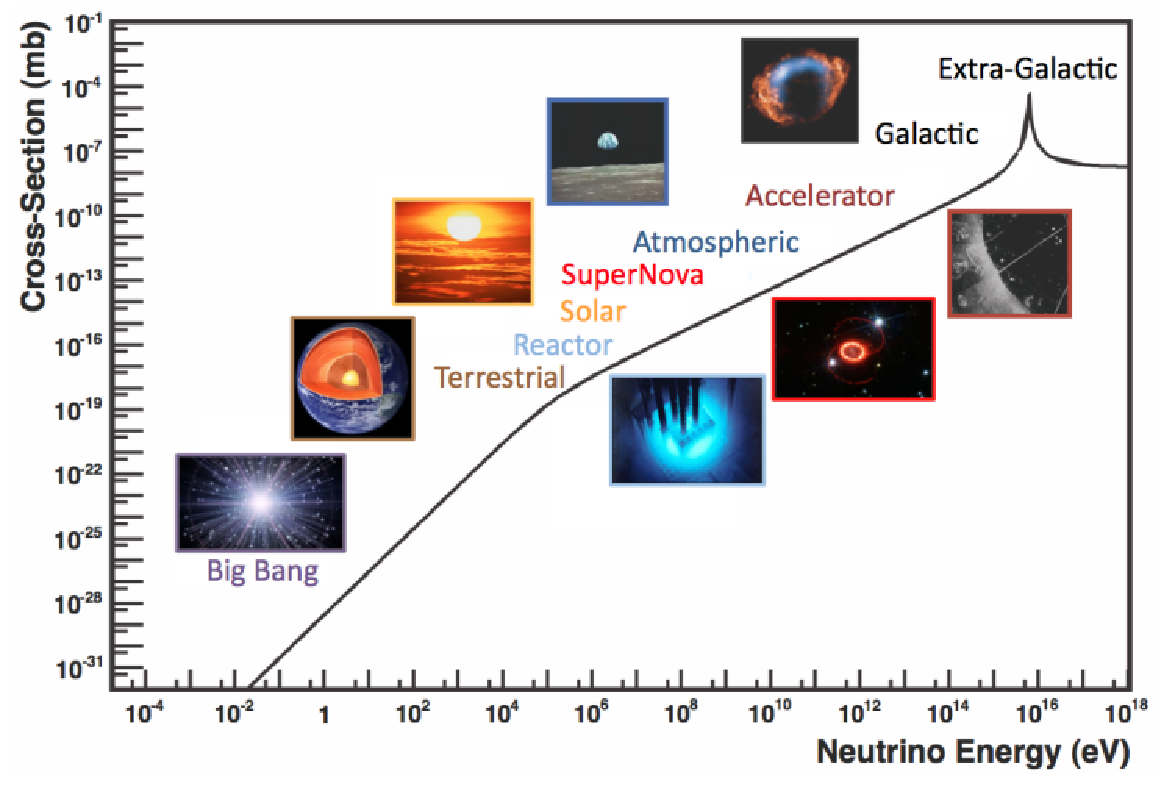
\includegraphics[width=\textwidth, trim={0mm 0mm 0mm 0mm}, clip,page=1]{Figures/Theory/EnergySpectrum.pdf}
  \end{subfigure}
  \caption{The cross-section of neutrinos from various natural and man-made sources as a function of neutrino energy. Taken from \cite{Formaggio:2012cpf}}
  \label{fig:NeutrinoOscillationPhysics_EnergySpectrum}
\end{figure}

\subsection{Solar Neutrinos}
\label{subsec:NeutrinoOscillationPhysics_SolarNeutrinos}

Solar neutrinos are emitted from fusion reaction chains at the center of the Sun. The solar neutrino flux, given as a function of neutrino energy for different fusion and decay chains, is illustrated in \autoref{fig:NeutrinoOscillationPhysics_SolarNeutrinoFlux}. Whilst proton-proton fusion generates the largest flux of neutrinos, the neutrinos are of low energy and are difficult to reconstruct due to the IBD interaction threshold of \quickmath{1.8\text{MeV}}. Consequently, most experiments focus on the neutrinos from the decay of \quickmath{^{8}B} (via \quickmath{^{8}B \rightarrow ^{8}Be^{*} + e^{+} + \nu_{e}}), which are higher energy.

\begin{figure}[h]
  \begin{subfigure}[t]{0.80\textwidth}
    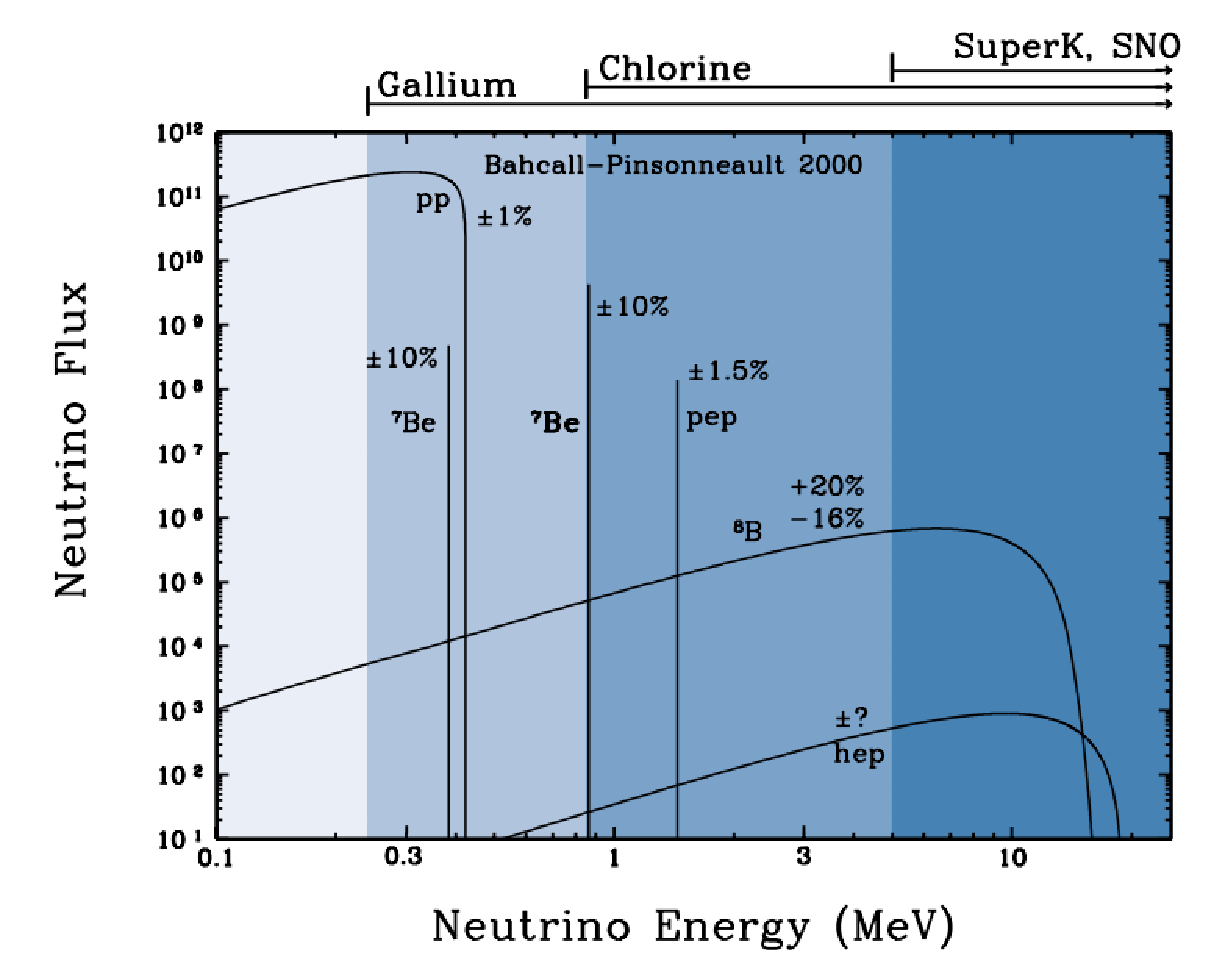
\includegraphics[width=\textwidth, trim={0mm 0mm 0mm 0mm}, clip,page=1]{Figures/Theory/SolarNeutrinoFlux.pdf}
  \end{subfigure}
  \caption{The solar neutrino flux as a function of neutrino energy for various fusion reactions and decay chains as predicted by the Standard Solar Model. Taken from \cite{Bellerive2004-ur}.}
  \label{fig:NeutrinoOscillationPhysics_SolarNeutrinoFlux}
\end{figure}

The first measurements of solar neutrinos observed a significant reduction in the event rate compared to predictions from the Standard Solar Model \cite{PhysRevLett.20.1205, Vinyoles2017-vv}. The proposed solution to this ``solar neutrino problem'' was \quickmath{\nu_{e} \leftrightarrow \nu_{\mu}} oscillations in a precursory version of the PMNS model \cite{Gribov1969-xi}. The Kamiokande \cite{PhysRevLett.63.16}, Gallex \cite{Hampel1999-of} and Sage \cite{PhysRevC.60.055801} experiments confirmed the \quickmath{\sim 0.5} factor deficit of solar neutrinos.

The conclusive solution to this problem was determined by the SNO collaboration \cite{Ahmad2002-zv}. Using a deuterium water target to observe \quickmath{^{8}B} neutrinos, the event rate of charged current (CC), neutral current (NC), and elastic scattering (ES) interactions (Given in \autoref{eq:NeutrinoOscillationPhysics_SNOInteractions}) was simultaneously measured. CC events can only occur for electron neutrinos, whereas the NC channel is agnostic to neutrino flavour, and the ES reaction has a slight excess sensitivity to electron neutrino interactions. This meant that there were direct measurements of the \quickmath{\nu_{e}} and \quickmath{\nu_x} neutrino flux. It was concluded that the CC and ES interaction rates were consistent with the deficit previously observed. Most importantly, the NC reaction rate was only consistent with the others under the hypothesis of flavour transformation.

\begin{equation}
  \label{eq:NeutrinoOscillationPhysics_SNOInteractions}
  \begin{split}
    \nu_{e} + d &\rightarrow p + p + e^{-} \hspace{2cm} (CC) \\
    \nu_{x} + d &\rightarrow p + n + \nu_{x} \hspace{2.02cm} (NC) \\
    \nu_{x} + e^{-} &\rightarrow \nu_{x} + e^{-} \hspace{2.55cm} (ES)
  \end{split}
\end{equation}

Many experiments have since measured the neutrino flux of different interaction chains within the sun \cite{Borexino_Collaboration2018-of, Aharmim2006-yb, Agostini2020-so}. The most recent measurement was that of CNO neutrinos which were recently observed with \quickmath{5\sigma} significance by the Borexino collaboration. Future neutrino experiments aim to further these spectroscopic measurements of different fusion chains within the Sun \cite{Andringa2016-zd, Beacom2017-ff, An2016-gm}. Solar neutrinos act as an irreducible background for dark matter experiments like DARWIN but oscillation parameter measurements can be made \cite{aalbers2020solar}.

\subsection{Atmospheric Neutrinos}
\label{subsec:NeutrinoOscillationPhysics_AtmosphericNeutrinos}

The interactions of primary cosmic ray protons in Earth's upper atmosphere generate showers of energetic hadrons. These are mostly pions and kaons which when they decay produce a natural source of neutrinos spanning energies of MeV to TeV \cite{Gaisser2002-gl}. The main decay is via

\begin{equation}
  \label{eq:NeutrinoOscillationPhysics_PionDecay}
  \begin{split}
    \pi^{\pm} &\rightarrow \mu^{\pm} + (\nu_{\mu},\bar{\nu}_\mu) \\
    \mu^{\pm} &\rightarrow e^{\pm} + (\nu_{\mu},\bar{\nu}_\mu) + (\nu_{e},\bar{\nu}_e)
  \end{split}
\end{equation}

such that for a single pion decay, three neutrinos are typically produced. The atmospheric neutrino flux energy spectra as predicted by the Bartol \cite{Barr_2004}, Honda \cite{Honda_2007, PhysRevD.70.043008, Honda:2011}, and FLUKA \cite{etde_20239111} models are illustrated in \autoref{fig:NeutrinoOscillationPhysics_AtmosphericNeutrinoFlux}. The flux distribution peaks at an energy of \quickmath{O(10) \text{GeV}}. The uncertainties associated with these models are dominated by the hadronic production of kaon and pions as well as the primary cosmic flux. 

\begin{figure}[h]
  \begin{subfigure}[t]{0.80\textwidth}
    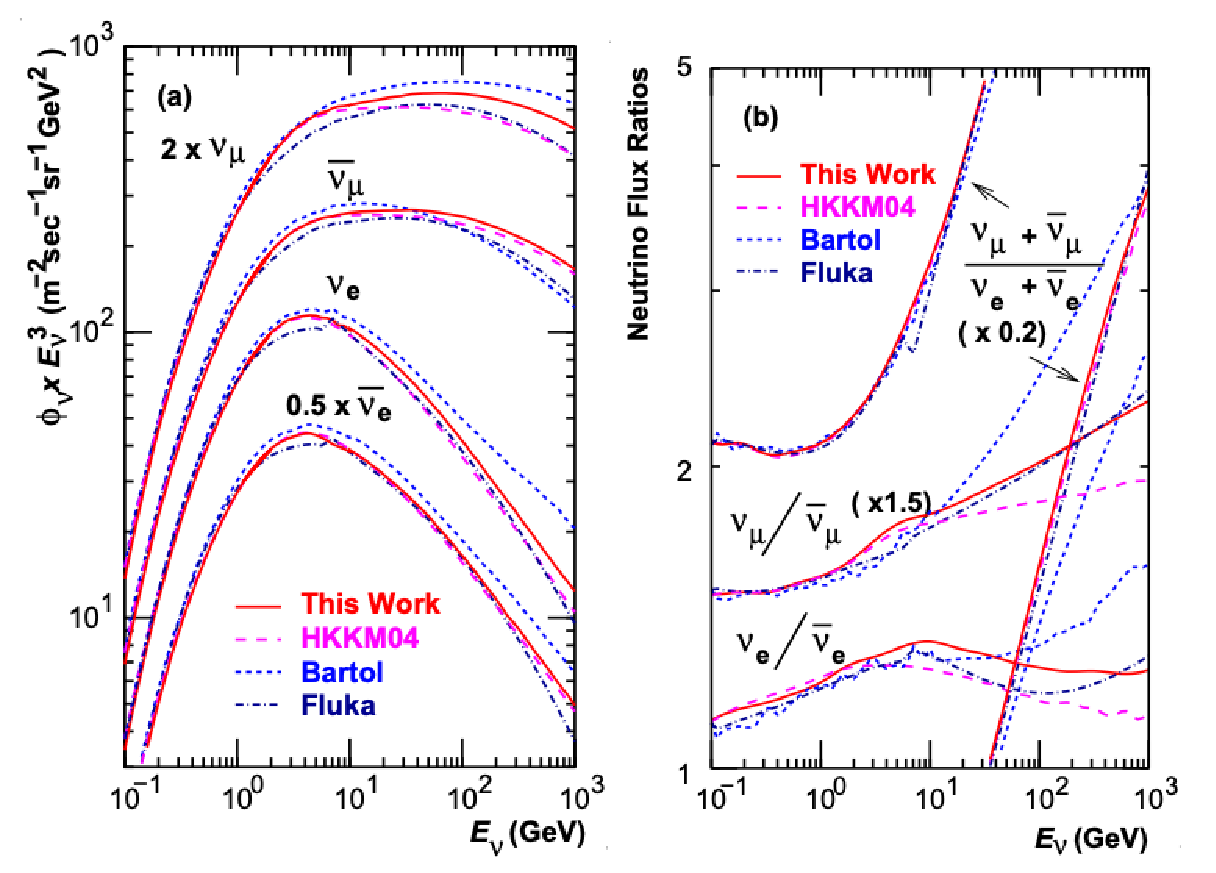
\includegraphics[width=\textwidth, trim={0mm 0mm 0mm 0mm}, clip,page=1]{Figures/Theory/AtmosphericNuFlux.pdf}
  \end{subfigure}
  \caption{Left panel: The atmospheric neutrino flux for different neutrino flavours as a function of neutrino energy as predicted by the 2007 Honda model (``This work'') \cite{Honda_2007}, the 2004 Honda model (``HKKM04'')\cite{PhysRevD.70.043008}, the Bartol model \cite{Barr_2004} and the FLUKA model \cite{etde_20239111}. Right panel: The ratio of the muon to electron neutrino flux as predicted by all the quoted models. Both figures taken from \cite{Honda_2007}.}
  \label{fig:NeutrinoOscillationPhysics_AtmosphericNeutrinoFlux}
\end{figure}

Unlike long-baseline experiments which have a fixed baseline, the distance atmospheric neutrinos propagate is dependent upon the zenith angle at which they interact. This is illustrated in \autoref{fig:NeutrinoOscillationPhysics_ZenithAngle}. Neutrinos that are generated directly above the detector (\quickmath{\cos(\theta)=1.0}) have a baseline equivalent to the height of the atmosphere whereas neutrinos that interact directly below the detector (\quickmath{\cos(\theta)=-1.0}) have to travel a length equal to the diameter of the  Earth. This means atmospheric neutrinos have a baseline that varies from \quickmath{O(20)\text{km}} to \quickmath{O(6 \times 10^{3})\text{km}}. Any neutrino generated at or below the horizon will be subject to matter effects as they propagate through the Earth.

\begin{figure}[h]
  \begin{subfigure}[t]{0.40\textwidth}
    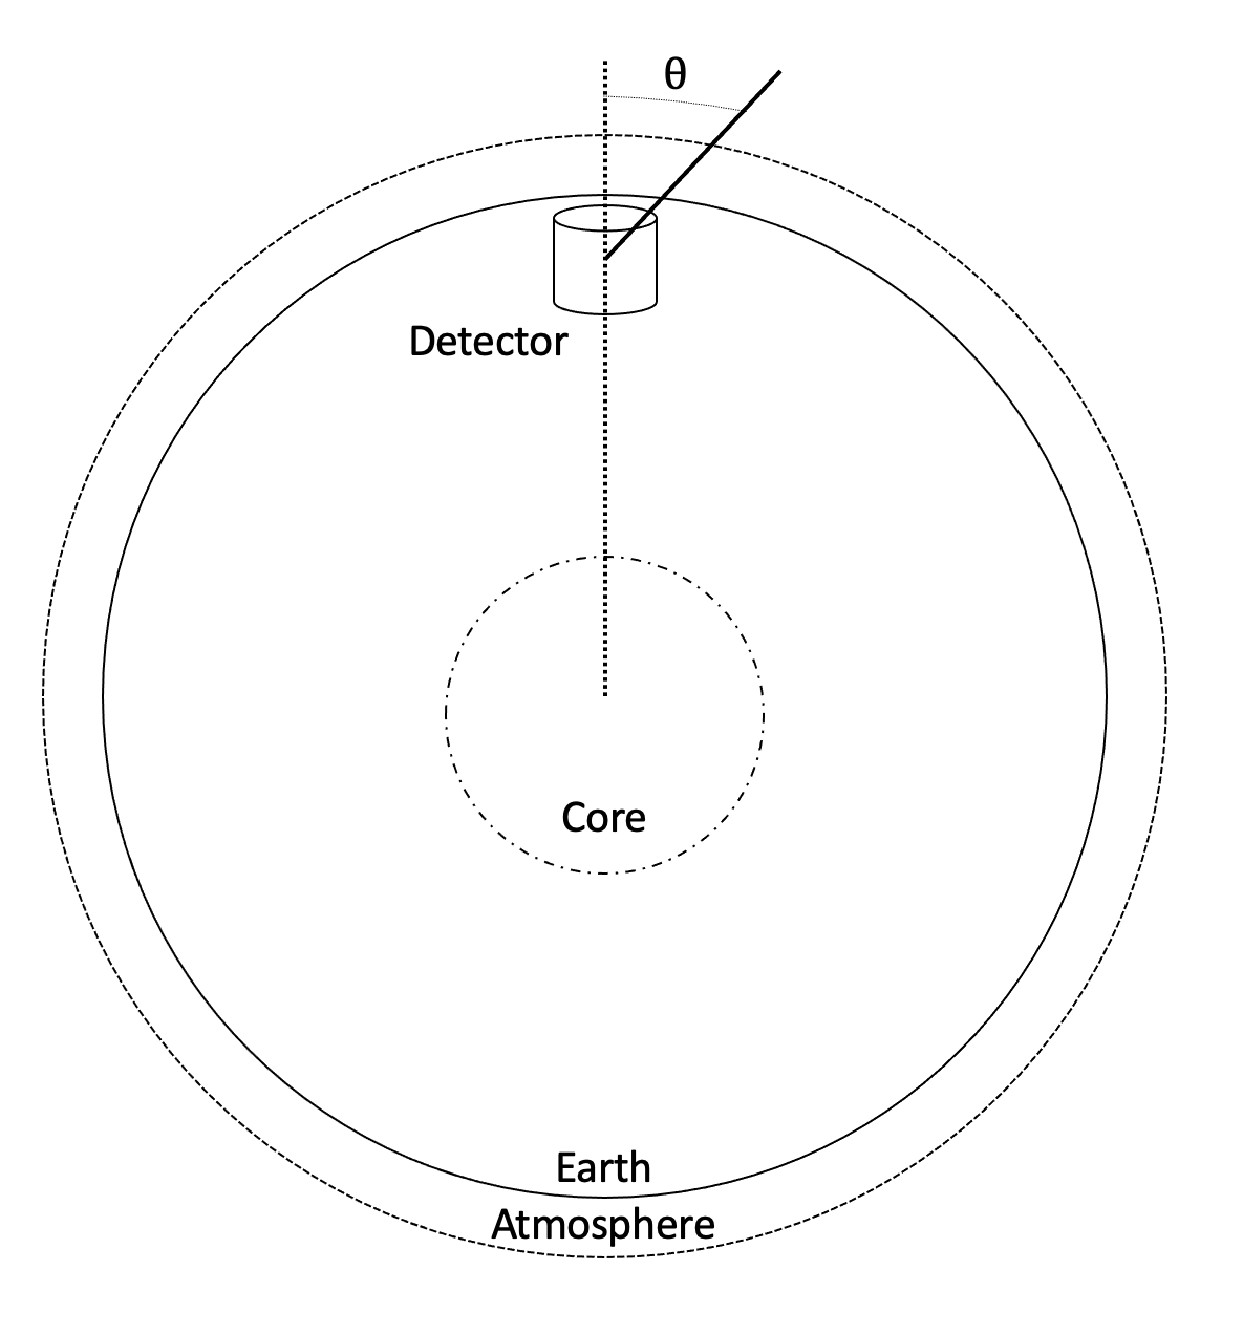
\includegraphics[width=\textwidth, trim={0mm 0mm 0mm 0mm}, clip,page=1]{Figures/Theory/ZenithAngle.pdf}
  \end{subfigure}
  \caption{A diagram illustrating the definition of zenith angle as used in the Super Kamiokande experiment \cite{Ashie_2005}.}
  \label{fig:NeutrinoOscillationPhysics_ZenithAngle}
\end{figure}

\autoref{fig:NeutrinoOscillationPhysics_NuFluxZenithAngleDep} highlights the neutrino flux as a function of the zenith angle for different slices of neutrino energy. For medium to high-energy neutrinos (and to a lesser degree for low-energy neutrinos), the flux is approximately symmetric around \quickmath{\cos(\theta)=0}. To the accuracy of this approximation, the systematic uncertainties associated with atmospheric flux for comparing upward-going and down-going neutrino cancels. This allows the down-going events, which are mostly insensitive to oscillation probabilities, to act as an unoscillated prediction (similar to a near detector in an accelerator neutrino experiment).

\begin{figure}[h]
  \begin{subfigure}[t]{0.90\textwidth}
    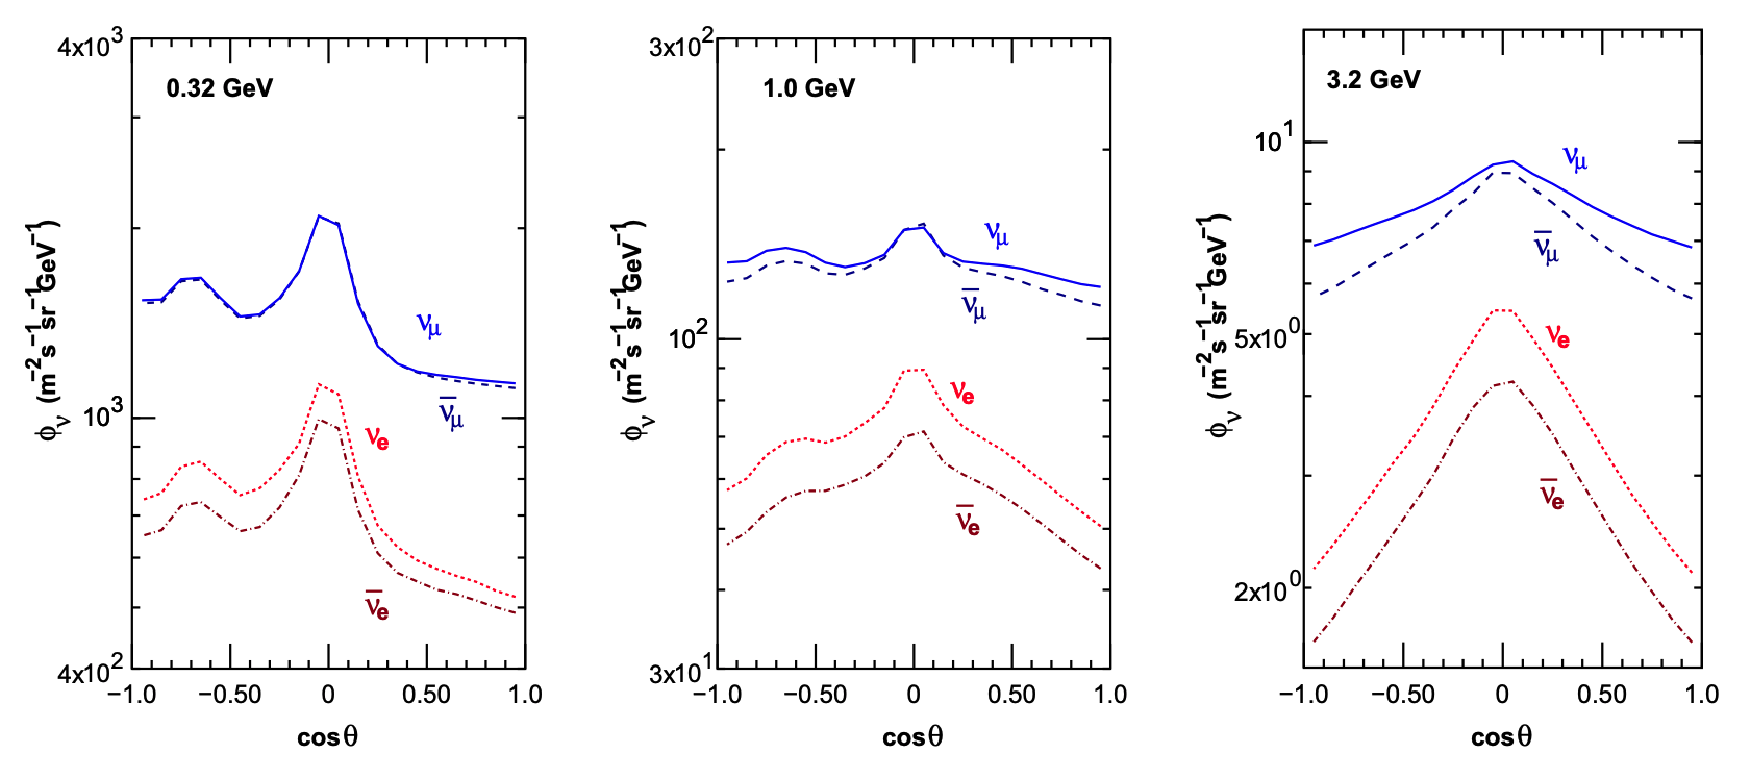
\includegraphics[width=\textwidth, trim={0mm 0mm 0mm 0mm}, clip,page=1]{Figures/Theory/NuFluxZenithAngleDep.pdf}
  \end{subfigure}
  \caption{Prediction of \quickmath{\nu_e, \bar{\nu}_{e}, \nu_{\mu}, \bar{\nu}_{\mu}} fluxes as a function of zenith angle as calculated by the HKKM model \cite{Honda:2011}. The left, middle and right panels represent three values of neutrino energy, \quickmath{0.32\text{GeV}}, \quickmath{1.0\text{GeV}} and \quickmath{3.2\text{GeV}} respectively. Predictions for other models including Bartol \cite{Barr_2004}, Honda \cite{Honda_2007} and FLUKA \cite{etde_20239111} are given in \cite{Ashie_2005}.}
  \label{fig:NeutrinoOscillationPhysics_NuFluxZenithAngleDep}
\end{figure}

Precursory hints of atmospheric neutrinos were observed in the mid-1960s searching for \quickmath{\overset{(-)}{\nu_\mu} + X \rightarrow X^{*} + \mu^{\pm}} \cite{Reines1965-cf}, although it was called an anomaly at the time of measurement. This was succeeded with the IMB-3 \cite{PhysRevLett.66.2561} and Kamiokande \cite{Hirata1992-qz} experiments which measured the ratio of muon neutrinos compared to electron neutrinos \quickmath{R(\nu_{\mu}/\nu_{e})}. Both experiments were found to have a consistent deficit of muon neutrinos, with \quickmath{R(\nu_{\mu}/\nu_{e}) = 0.67 \pm 0.17} and \quickmath{R(\nu_{\mu}/\nu_{e}) = 0.60 \substack{+ 0.07 \\ -0.06} \pm 0.05}. %Soudan-2 \cite{Allison1997-qz} determined similar measurements.
Super-Kamiokande (SK) \cite{Ashie_2005} extended this analysis by fitting oscillation parameters in \quickmath{P(\nu_\mu \rightarrow \nu_\tau)} which found best fit parameters \quickmath{\sin^{2}(2\theta) > 0.92} and \quickmath{1.5 \times 10^{-3} < \Delta m^{2} < 3.4 \times 10^{-3} \text{eV}^{2}}.

Since then, atmospheric neutrino experiments have been making precision measurements of the \sinsqatm and \quickmath{\Delta m^{2}_{32}} oscillation parameters.
%, and to a lesser extent the sign of \delmsqatm through the matter resonance present for any neutrinos passing through the Earth.
Atmospheric neutrino oscillation is dominated by \quickmath{P(\nu_{\mu} \rightarrow \nu_{\tau})}, where SK observed a \quickmath{4.6\sigma} discovery of \quickmath{\nu_{\tau}} appearance \cite{Li_2018}. \autoref{fig:NeutrinoOscillationPhysics_AtmosphericParamContour} illustrates the current estimates on the atmospheric mixing parameters from a wide range of atmospheric and accelerator neutrino observatories.

\begin{figure}[h]
  \begin{subfigure}[t]{0.90\textwidth}
    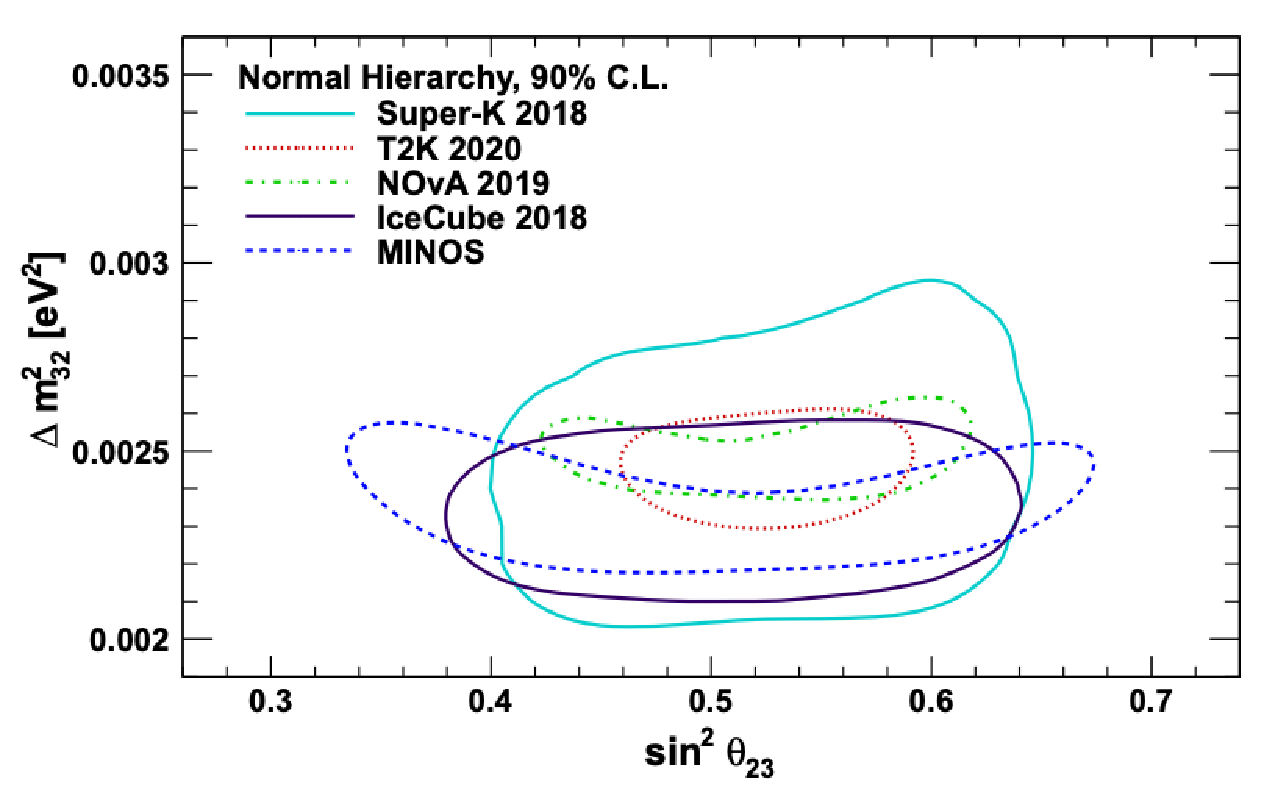
\includegraphics[width=\textwidth, trim={0mm 0mm 0mm 0mm}, clip,page=1]{Figures/Theory/AtmosphericParams.pdf}
  \end{subfigure}
  \caption{Constraints on the atmospheric oscillation parameters, \sinsqatm and \delmsqatm, from atmospheric and long baseline experiments: SK \cite{Kamiokande_Collaboration2017-nf}, T2K \cite{T2K_Collaboration2018-sm}, \quickmath{\text{NO}\nu\text{A}} \cite{Acero2019-rw}, IceCube \cite{Aartsen2018-cz} and MINOS \cite{Adamson2014-tt}. Figure taken from \cite{Athar_2022}.}
  \label{fig:NeutrinoOscillationPhysics_AtmosphericParamContour}
\end{figure}

\subsection{Accelerator Neutrinos}
\label{subsec:NeutrinoOscillationPhysics_AcceleratorNeutrinos}

The concept of using a man-made ``neutrino beam'' was first realised in 1962 \cite{Danby1962-ph}.
%and led to the first discovery that \quickmath{\nu_{e}} and \quickmath{\nu_{\mu}} were in fact different particles.
Since then, many experiments have followed which all use the same fundamental concepts. Typically, a proton beam is aimed at a target producing charged mesons that decay to neutrinos. The mesons can be sign-selected by the use of magnetic focusing horns to generate a neutrino or antineutrino beam.
%Absorbing material and the rock between the target and detector absorb all particles barring the neutrinos.
Pions are the primary meson that decay and depending on the orientation of the magnetic field, a muon (anti-)neutrino beam is generated via \quickmath{\pi^{+} \rightarrow \mu^{+} + \nu_{\mu}} or \quickmath{\pi^{-} \rightarrow \mu^{-} + \bar{\nu}_{\mu}}. The decay of muons and kaons does result in an irreducible intrinsic electron neutrino background. In T2K, this background contamination is \quickmath{O(<1\%)} \cite{Abe_2013}. There is also an approximately \quickmath{\sim 5\%} ``wrong-sign'' neutrino background of \quickmath{\bar{\nu}_{\mu}} generated via the same decays. As the beam is generated by proton interactions (rather than anti-proton interactions), the wrong-sign component in the antineutrino beam is larger when operating in neutrino mode.

Tuning the proton energy in the beam and using beam focusing techniques allows the neutrino energy to be set to a value that maximises the disappearance oscillation probability in the \quickmath{L/E} term in \autoref{eq:NeutrinoOscillationPhysics_PMNS_2FlavourOscProb}.
%As the inital proton beam can be tuned resulting in a tunable neutrino energy spectra, the advantage of these type of experiments is that they can be focused in on the oscillation dip presented by the \quickmath{L/E} term in \autoref{eq:NeutrinoOscillationPhysics_PMNS_2FlavourOscProb} using the two flavour approximation.
This means that accelerator experiments are typically more sensitive to the mixing parameters as compared to a natural neutrino source. However, the disadvantage compared to atmospheric neutrino experiments is that the baseline has to be shorter due to the lower flux. Consequently, there is typically less sensitivity to matter effects and the ordering of the neutrino mass eigenstates.

A neutrino experiment measures

\begin{equation}
  \label{eq:NeutrinoOscillationPhysics_DetectorMeasurement}
  R(\vec{x}) = \Phi(E_{\nu}) \times \sigma(E_{\nu}) \times \epsilon(\vec{x}) \times P(\nu_{\alpha} \rightarrow \nu_{\beta}),
\end{equation}

where \quickmath{R(\vec{x})} is the event rate of neutrinos at position \quickmath{\vec{x}}, \quickmath{\Phi(E_{\nu})} is the flux of neutrinos with energy \quickmath{E_{\nu}}, \quickmath{\sigma(E_{\nu})} is the cross-section of the neutrino interaction and \quickmath{\epsilon(\vec{x})} is the efficiency and resolution of the detector. In order to leverage the most out of an accelerator neutrino experiment, the flux and cross-section systematics need to be constrained. This is typically done via the use of a ``near detector'', situated at a baseline of \quickmath{O(1)\text{km}}. This detector observes the unoscillated neutrino flux and constrains the parameters used within the flux and cross-section model.

The first accelerator experiments to precisely measure oscillation parameters were MINOS \cite{PhysRevLett.97.191801} and K2K \cite{PhysRevLett.9.36}.
These experiments confirmed the \quickmath{\nu_{\mu}} disappearance seen in atmospheric neutrino experiments by finding consistent parameter values for \sinsqatm and \delmsqatm.
The current generation of accelerator neutrino experiments, T2K and \NOVA extended this field by observing \quickmath{\bar{\nu}_{\mu} \rightarrow \bar{\nu}_{e}} and lead the sensitivity to atmospheric mixing parameters as seen in \autoref{fig:NeutrinoOscillationPhysics_AtmosphericParamContour} \cite{PhysRevLett.123.151803}.
The two experiments differ in their peak neutrino energy, baseline, and detection technique.
The \NOVA experiment is situated at a baseline of \quickmath{810\text{km}} from the NuMI beamline which delivers \quickmath{2\text{GeV}} neutrinos.
The T2K neutrino beam is peaked around \quickmath{0.6 \text{GeV}} and propagates \quickmath{295\text{km}}.
The \NOVA experiment also uses functionally identical detectors (near and far) which allow the approximate cancellation of detector systematics whereas T2K uses a plastic scintillator technique at the near detector and a water Cherenkov far detector.
The future generation experiments DUNE \cite{Abi2020-cm} and Hyper-Kamiokande \cite{Hyper-Kamiokande_Proto-Collaboration2015-ac} will succeed these experiments as the high-precision era of neutrino oscillation parameter measurements develops.

Several anomalous results have been observed in the LSND \cite{PhysRevD.64.112007} and MiniBooNE \cite{PhysRevLett.110.161801} detectors which were designed with purposefully short baselines. Parts of the neutrino community attributed these results to oscillations induced by a fourth ``sterile'' neutrino \cite{Blanco_2020} but several searches in other experiments, MicroBooNE \cite{10.48550/arxiv.2110.14054} and KARMEN \cite{PhysRevD.65.112001}, found no hints of additional neutrino species. The solution to the anomalous results is still being determined.

\subsection{Reactor Neutrinos}
\label{subsec:NeutrinoOscillationPhysics_ReactorNeutrinos}

As illustrated in the first discovery of neutrinos (\autoref{sec:NeutrinoOscillationPhysics_Discovery}), nuclear reactors are a very useful man-made source of electron antineutrinos. For reactors that use low-enriched uranium \quickmath{^{235}\text{U}} as fuel, the antineutrino flux is dominated by the \quickmath{\beta}-decay fission of \quickmath{^{235}\text{U}}, \quickmath{^{238}\text{U}}, \quickmath{^{239}\text{Pu}} and \quickmath{^{241}\text{Pu}} \cite{Kim2013-ye} as illustrated in \autoref{fig:NeutrinoOscillationPhysics_ReactorNeutrinoProduction}.

\begin{figure}[h]
  \begin{subfigure}[t]{0.90\textwidth}
    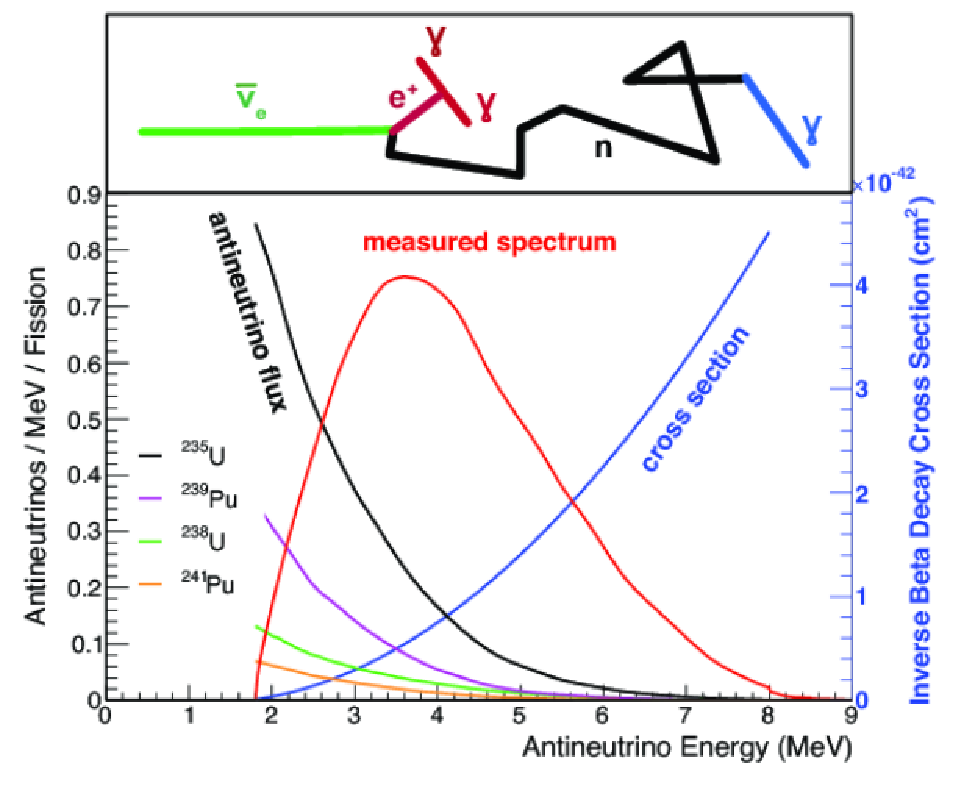
\includegraphics[width=\textwidth, trim={0mm 0mm 0mm 0mm}, clip,page=1]{Figures/Theory/ReactorNeutrinoProduction.pdf}
  \end{subfigure}
  \caption{Reactor electron antineutrino fluxes for \quickmath{^{235}\text{U}} (Black), \quickmath{^{238}\text{U}} (Green), \quickmath{^{239}\text{Pu}} (Purple), and \quickmath{^{241}\text{Pu}} (Orange) isotopes. The inverse \quickmath{\beta}-decay cross-section (Blue) and corresponding measurable neutrino spectrum (Red) are also given. Top panel: Schematic of Inverse \quickmath{\beta}-decay interaction including the eventual capture of the emitted neutron. This capture emits a \quickmath{\gamma}-ray which provides a second signal of the event. Taken from \cite{SajjadAthar:2021prg}.}
  \label{fig:NeutrinoOscillationPhysics_ReactorNeutrinoProduction}
\end{figure}

Due to their low energy, reactor electron antineutrinos predominantly interact via the inverse \quickmath{\beta}-decay (IBD) interaction. The typical signature contains two signals delayed by \quickmath{O(200)\mu\text{s}}; firstly the prompt photons from positron annihilation, and secondly the photons emitted (\quickmath{E_{tot}^{\gamma} = 2.2\text{MeV}}) from de-excitation after neutron capture on hydrogen. Searching for both signals improves the detector's ability to distinguish between background and signal events \cite{Abe2022-ij}. Recently, SK included gadolinium dopants into the ultra-pure water to increase the energy released from the photon cascade to \quickmath{\sim 8\text{MeV}} and reduce the time of the delayed signal to \quickmath{\sim 28 \mu \text{s}}.

There are many short baseline experiments (\quickmath{\text{L} \sim O(1)\text{km}}) that have measured the \sinsqreac and \delmsqatm oscillation parameters. Daya Bay \cite{PhysRevLett.108.171803}, RENO \cite{PhysRevLett.108.191802} and Double Chooz \cite{PhysRevLett.108.131801} have all provided precise measurements, with the first discovery of a non-zero \quickmath{\theta_{13}} made by Daya Bay and RENO (and complemented by T2K \cite{PhysRevLett.108.131801}). The constraints on \sinsqreac by the reactor experiments lead the field and are often used as external inputs to accelerator neutrino experiments to improve their sensitivity to \dcp and mass hierarchy determination.
%One curiosity of these short baseline reactor experiments is the `\quickmath{5 \text{MeV}} excess' \cite{Berryman_2019}. First observed in 2014 \cite{For_the_RENO_Collaboration2015-zy, Abe_2014}, all three experiments listed observed a shape excess in events around \quickmath{E_{\nu} \sim 5 \text{MeV}}. The reason behind this excess is speculated to be either oscillations to sterile neutrinos or a fault in the Huber-Mueller model \cite{Mueller_2011}. At this time, the latter is favoured as Daya Bay \cite{PhysRevLett.123.111801} observed substantial evidence (\quickmath{4.0\sigma}) of correlation between the excess and the \quickmath{^{235}\text{U}} electron antineutrino flux.
%Other neutrino experiments, PROSPECT \cite{PhysRevD.103.032001} and STEREO \cite{STEREO} show similar results data to help determine the cause of the excess.
JUNO-TAO \cite{junocollaboration2020tao}, a small collaboration within the larger JUNO experiment, is a next-generation reactor experiment that aims to precisely measure the isotopic antineutrino yields from the different fission chains. Alongside this, it aims to explain the `\quickmath{5 \text{MeV}} excess' \cite{For_the_RENO_Collaboration2015-zy, Abe_2014, PhysRevLett.123.111801} by conducting a search for sterile neutrinos with a mass scale of around \quickmath{1 \text{eV}}.

Kamland \cite{Decowski2016-hh} is the only experiment to have observed reactor neutrinos using a long baseline (flux weighted averaged baseline of \quickmath{L \sim 180\text{km}}) which allows it to have sensitivity to \delmsqsol. Combined with the SK solar neutrino experiment, the combined analysis puts the most stringent constraint on \delmsqsol \cite{PhysRevD.83.052002}.

\section{Summary}
\label{sec:Theory_Summary}

Since observing the first evidence of neutrino oscillations in the late 1990's, numerous measurements of the mixing parameters have been made. Many experiments use neutrinos as a tool for discovery of new physics (diffuse supernoave background, neutrinoless double beta decay and others) so the PMNS parameters are summarised in the Particle Data Group (PDG) review tables. The analysis presented in this thesis focuses on the 2020 T2K oscillation analysis presented in \cite{Dunne2020-uf} where the 2018 PDG constraints \cite{Tanabashi2018-hp} were used. These constraints are outlined in \autoref{tab:Theory_PDGConstraints}.

\begin{table}[ht!]
    \centering
    \begin{tabular}{c|c}
      \hline
      Parameter & 2018 Constraint \\
      \hline
      \quickmath{\sin^{2}(\theta_{12})} & \quickmath{0.307 \pm 0.013} \\
      \quickmath{\Delta m^{2}_{21}} & \quickmath{(7.53 \pm 0.18) \times 10^{-5} \text{eV}^{2}} \\
      \quickmath{\sin^{2}(\theta_{13})} & \quickmath{(2.12 \pm 0.08) \times 10^{-2}} \\
      \quickmath{\sin^{2}(\theta_{23})} (I.H., Q1) & \quickmath{0.421^{+0.033}_{-0.025}} \\
      \quickmath{\sin^{2}(\theta_{23})} (I.H., Q2) & \quickmath{0.592^{+0.023}_{-0.030}} \\
      \quickmath{\sin^{2}(\theta_{23})} (N.H., Q1) & \quickmath{0.417^{+0.025}_{-0.028}} \\
      \quickmath{\sin^{2}(\theta_{23})} (N.H., Q2) & \quickmath{0.597^{+0.024}_{-0.030}} \\
      \quickmath{\Delta m^{2}_{32}} (I.H.) & \quickmath{(-2.56 \pm 0.04) \times 10^{-3} \text{eV}^{2}} \\
      \quickmath{\Delta m^{2}_{32}} (N.H.) & \quickmath{(2.51 \pm 0.05) \times 10^{-3} \text{eV}^{2}} \\
      \hline
      \hline
    \end{tabular}
    \caption{The 2018 Particle Data Group constraints of the oscillation parameters taken from \cite{Tanabashi2018-hp}. The value of \delmsqatm is given for both normal hierarchy (N.H.) and inverted hierarchy (I.H.) and \sinsqatm is broken down by whether its value is below (Q1) or above (Q2) \quickmath{0.5}.}
    \label{tab:Theory_PDGConstraints}
\end{table}

The \sinsqreac measurement stems from the electron antineutrino disappearance, \quickmath{P(\bar{\nu}_{e} \rightarrow \bar{\nu}_{e})}, and is take as the  average best-fit from the combination of Daya Bay, Reno and Double Chooz. It is often used as a prior uncertainty within other neutrino oscillation experiments, typically termed the reactor constraint. The \sinsqsol parameter is predominantely measured through electron neutrino disappearance, \quickmath{P(\nu_{e} \rightarrow \nu_{\mu,\tau})}, in solar neutrino experiments. The long-baseline reactor neutrino experiment Kamland also has sensitivity to this parameter and is used in a joint fit to solar data from SNO and SK, using the reactor constraint. Measurements of \sinsqatm are made by long-baseline and atmospheric neutrino experiments. The PDG value is a joint fit of T2K, \NOVA, MINOS and IceCube DeepCore experiments. The latest T2K-only meaurement, provided at Neutrino2020 and is the basis of this thesis, is given as \quickmath{\sin^{2}(\theta_{23}) = 0.546^{+0.024}_{-0.046}} \cite{Dunne2020-uf}. The PDG constraint on \delmsqsol is provided by the KamLAND experiment using solar and geoneutrino data. This measurement utilised a \sinsqreac constraint from accelerator (T2K, MINOS) and reactor neutrino (Daya Bay, RENO, Double Chooz) experiments. Accelerator measurements make some of the most stringent constraints on \delmsqatm although atmospheric experiments have more sensitivity to the mass hierarchy determination. The PDG performs a joint fit of accelerator and atmospheric data, in both normal and inverted hierarchy separately. The latest T2K-only result is \quickmath{\Delta m^{2}_{32} = 2.49^{+0.058}_{-0.082} \times 10^{-3}\text{eV}^{2}} favouring normal hierarchy \cite{Dunne2020-uf}. The value of \dcp is largely undetermined. CP-conserving values of \quickmath{0} and \quickmath{\pi} were rejected with \quickmath{\sim 2\sigma} intervals, as published in Nature, although more recent analysis have reduced the rejection intervals to \quickmath{90\%}. Since the 2018 PDG publication, there has been a new measurement of \quickmath{\sin^{2}(\theta_{13}) = (2.20 \pm 0.07) \times 10^{-2}} \cite{Workman:2022ynf}, alongside updated \delmsqatm and \sinsqatm measurements.

Throughout this thesis, several sample spectra predictions and contours are presented which require oscillation parameters to be assumed. \autoref{tab:Theory_ParameterSets} defines two sets of oscillation parameters, with ``Asimov A'' set being close to the preferred values from a previous T2K-only fit \cite{PhysRevLett.112.181801} and ``Asimov B'' being CP-conserving and further from maximal \quickmath{\theta_{23}} mixing.

\begin{table}[ht!]
    \centering
    \begin{tabular}{c|c|c}
      \hline
      \hline
      Parameter & Asimov A & Asimov B \\
      \hline
      \quickmath{\Delta m^{2}_{12}} & \multicolumn{2}{c}{\quickmath{7.53 \times 10^{-5} \text{eV}^{2}}} \\ \hline
      \quickmath{\Delta m^{2}_{32}} & \multicolumn{2}{c}{\quickmath{2.509 \times 10^{-3} \text{eV}^{2}}} \\ \hline
      \quickmath{\sin^{2}\left(\theta_{12}\right)} & \multicolumn{2}{c}{\quickmath{0.304}} \\ \hline
      \quickmath{\sin^{2}\left(\theta_{13}\right)} & \multicolumn{2}{c}{\quickmath{0.0219}} \\ \hline
      \quickmath{\sin^{2}\left(\theta_{23}\right)} & \quickmath{0.528} & \quickmath{0.45} \\ \hline
      \quickmath{\delta_{CP}} & \quickmath{-1.601} & \quickmath{0.0} \\ \hline
      \hline
    \end{tabular}
    \caption{Reference values of the neutrino oscillation parameters for two different oscillation parameter sets.}
    \label{tab:Theory_ParameterSets}
\end{table}

  \chapter{Super Kamiokande}
\label{chap:SuperKamiokande}
Super Kamiokande Chapter

\section{Overview}
\label{sec:SuperKamiokande_Overview}
Super Kamiokande Overview Section

\section{Cerenkov Radiation}
\label{sec:SuperKamiokande_CerenkovRadiation}
Super Kamiokande Cerenkov Radiation Section

\section{Detector}
\label{sec:SuperKamiokande_Detector}
Super Kamiokande Detector Section

\section{Electronics}
\label{sec:SuperKamiokande_Electronics}
Super Kamiokande Electronics Section

\section{Calibration}
\label{sec:SuperKamiokande_Calibration}
Super Kamiokande Calibration Section

  \chapter{T2K}
\label{chap:T2K}
T2K Chapter

\section{Overview}
\label{sec:T2K_Overview}
T2K Overview Section

\section{Neutrino Beamline}
\label{sec:T2K_Beamline}
T2K Neutrino Beamline Section

\section{Neutrino Flux}
\label{sec:T2K_NeutrinoFlux}
T2K Neutrino Flux Section

\section{Detectors}
\label{sec:T2K_Detectors}
T2K Detectors Section

\subsection{ND280}
\label{sec:T2K_ND280}
T2K ND280 SubSection

\subsection{INGRID}
\label{sec:T2K_INGRID}
T2K INGRID SubSection

  \chapter{Bayesian Statistics and Markov Chain Monte Carlo Techniques}
\label{chap:MarkovChainMonteCarlo}
This thesis presents a Bayesian oscillation analysis. To extract the oscillation parameters, a Markov Chain Monte Carlo (MCMC) method is used. This chapter explains the theory of how parameter estimates can be determined using this technique and condenses the material found in the literature \cite{mcmc_handbook, mcmc_practice, thesis_clarence, thesis_kirsty}.

The oscillation parameter determination presented here is built upon a simultaneous fit to neutrino beam data in the near detector, beam data at SK, and atmospheric data at SK. In total, there are four oscillation parameters of interest (\quickmath{\sin^{2}(\theta_{23})}, \quickmath{\sin^{2}(\theta_{13})}, \quickmath{\Delta m^{2}_{32}}, and \quickmath{\delta_{CP}}), two oscillation parameters to which this study will not be sensitive (\quickmath{\sin^{2}(\theta_{12})}, \quickmath{\Delta m^{2}_{21}}) and  many nuisance parameters that control the systematic uncertainty models.
%The systematic uncertainties can be grouped into categories depending on how they are defined: $574$ bin-normalisations due to the near detector response, $45$ bin-normalisations to describe the far detector response to neutrino beam events, $27$ parameters to describe the detector response to atmospheric neutrino events, $100$ to model the bin-normalisation due to beam flux uncertainties, $18$ which model the atmospheric flux uncertainties, and $87$ to describe the correlated cross-section model. An alternative parameterisation, where the far detector response is correlated between the beam and atmospheric samples, replaces the bin-normalisation parameters with $224$ shift and smear systematics. Section Link to Systematics Chapter describes the systematic model in more depth.

This analysis uses a Monte Carlo technique to generate a multi-dimensional probability distribution across all of the model parameters used in the fit. To determine an estimate for each parameter, this multi-dimensional object is integrated over all other parameters. This process is called Marginalisation and is described in \autoref{sec:MarkovChainMonteCarlo_Marginalisation}. Monte Carlo techniques approximate the probability distribution of each parameter within the limit of generating infinite samples. As ever, generating a large number of samples is time and resource-dependent. Therefore, an MCMC technique is utilised within this analysis to reduce the required number of steps to sufficiently sample the parameter space. This technique is described in further detail in \autoref{sec:MarkovChainMonteCarlo_MarkovChainMC}.

\finish{Introduce MaCh3 and say what I did on it}

\section{Bayesian Statistics}
\label{sec:MarkovChainMonteCarlo_BayesianStatistics}

Bayesian inference treats observable data, \quickmath{D}, and model parameters, \quickmath{\vec{\theta}}, on equal footing such that a probability model of both data and parameters is required. This is the joint probability distribution \quickmath{P(D, \vec{\theta})} and can be described by the prior distribution for model parameters \quickmath{P(\vec{\theta})} and the likelihood of the data given the model parameters \quickmath{P(D|\vec{\theta})},

\begin{equation}
  P(D,\vec{\theta}) = P(D|\vec{\theta})P(\vec{\theta}).
\end{equation}

The prior distribution, \quickmath{P(\vec{\theta})}, describes all previous knowledge about the parameters within the model. For example, if the risk of developing health problems is known to increase with age, the prior distribution would describe the increase. For the purpose of this analysis, the prior distribution is typically the best-fit values taken from external data measurements with a Gaussian uncertainty. The prior distribution can also contain correlations between model parameters. In an analysis using Monte Carlo techniques, the likelihood of measuring some data assuming some set of model parameters is calculated by comparing the Monte Carlo prediction generated at that particular set of model parameters to the data.

It is parameter estimation that is important for this analysis and as such, we apply Bayes' theorem \cite{Bayes:1764vd} to calculate the probability for each parameter to have a certain value given the observed data, \quickmath{P(\vec{\theta}|D)}, which is known as the posterior distribution (often termed the posterior). This can be expressed as

\begin{equation}
  \label{eq:MarkovChainMonteCarlo_PosteriorDistribution}
  P(\vec{\theta}|D) = \frac{ P(D|\vec{\theta}) P(\vec{\theta}) }{\int P(D|\vec{\theta}) P(\vec{\theta}) d\vec{\theta}}.
\end{equation}

The denominator in \autoref{eq:MarkovChainMonteCarlo_PosteriorDistribution} is the integral of the joint probability distribution over all values of all parameters used within the fit. For brevity, we say that the posterior distribution is

\begin{equation}
  \label{eq:MarkovChainMonteCarlo_PosteriorDistributionReduced}
  P(\vec{\theta}|D) \propto P(D|\vec{\theta}) P(\vec{\theta}).
\end{equation}

%In \autoref{sec:MarkovChainMonteCarlo_Marginalisation}, we see that for the cases used within this analysis, it is reasonable to know the posterior to some normalisation constant.
For the purposes of this analysis, it is acceptable to neglect the normalisation term and focus on this proportional relationship.

\subsection{Application of Prior Knowledge}
\label{sec:MarkovChainMonteCarlo_Priors}

The posterior distribution is proportional to the prior uncertainty applied to each parameter, as illustrated by \autoref{eq:MarkovChainMonteCarlo_PosteriorDistributionReduced}. This means that it is possible to change the prior after the posterior distribution has been determined. The prior uncertainty of a particular parameter can be `divided' out of the posterior distribution and the resulting distribution can be reweighted using the new prior uncertainty that is to be applied. The methodology and implementation of changing the prior follows that described in \cite{thesis_artur}. 

An example implementation that is useful for this analysis is the application of the ``reactor constraint''. As discussed in \autoref{sec:Theory_Summary}, an external constraint on \quickmath{\sin^{2}(\theta_{13})} is determined from measurements taken from reactor experiments. However, the sensitivities from just using the T2K and SK samples is equally as important. Without this technique, two fits would have to be run, doubling the required resources. Therefore, the key benefit for this analysis is the fact that only a single `fit' has to be performed and can be used to build the two posterior distributions of the with and without reactor constraint applied.

\section{Monte Carlo Simulation}
\label{sec:MarkovChainMonteCarlo_MonteCarloSimulation}
Monte Carlo techniques are used to numerically solve a complex problem that does not necessarily have an analytical solution. These techniques rely on building a large ensemble of samples from an unknown distribution and then using the ensemble to approximate the properties of the distribution.

An example that uses Monte Carlo techniques is to calculate the area underneath a curve. For example, take the problem of calculating the area under a straight line with gradient \quickmath{M = 0.4} and intercept \quickmath{C = 1.0}. Analytically, one can calculate the area under the line is equal to 30 units for \quickmath{0 \leq x \leq 10}. Using Monte Carlo techniques, one can calculate the area under this line by throwing many random values for the \quickmath{x} and \quickmath{y} components of each sample and then calculating whether that point falls below the line. The area can then be calculated by the ratio of points below the line to the total number of samples thrown multiplied by the total area in which samples were scattered. The study is shown in \autoref{fig:MCMC_MCTechnique} highlights this technique and finds the area under the curve to be \quickmath{29.9} compared to an analytical solution of \quickmath{30.0}. The deviation of the numerical to analytical solution can be attributed to the number of samples used in the study. The accuracy of the approximation in which the properties of the Monte Carlo samples replicate those of the desired distribution is dependent on the number of samples used. Replicating this study with a differing number of Monte Carlo samples used in each study (As shown in \autoref{fig:MCMC_MCTechniqueNThrowsStudy}) highlights how the Monte Carlo techniques are only accurate within the limit of a high number of samples.

Whilst the above example has an analytical solution, these techniques are just as applicable to complex solutions. Clearly,  any numerical solution is only as useful as its efficiency. As discussed, the accuracy of the Monte Carlo technique is dependent upon the number of samples generated to approximate the properties of the distribution. Furthermore, if the positions at which the samples are evaluated are not `cleverly' picked, the efficiency of the Monte Carlo technique significantly drops. Given the example in \autoref{fig:MCMC_MCTechnique}, if the region in which the samples are scattered significantly extends passed the region of interest, many calculations will be calculated but do not add to the ability of the Monte Carlo technique to achieve the correct result. For instance, any sample evaluated at a \quickmath{y \geq 5} could be removed without affecting the final result. This does bring in an aspect of the `chicken and egg' problem in that to achieve efficient sampling, one needs to know the distribution beforehand.

\begin{figure}[h]
  \begin{subfigure}[t]{0.80\textwidth}
    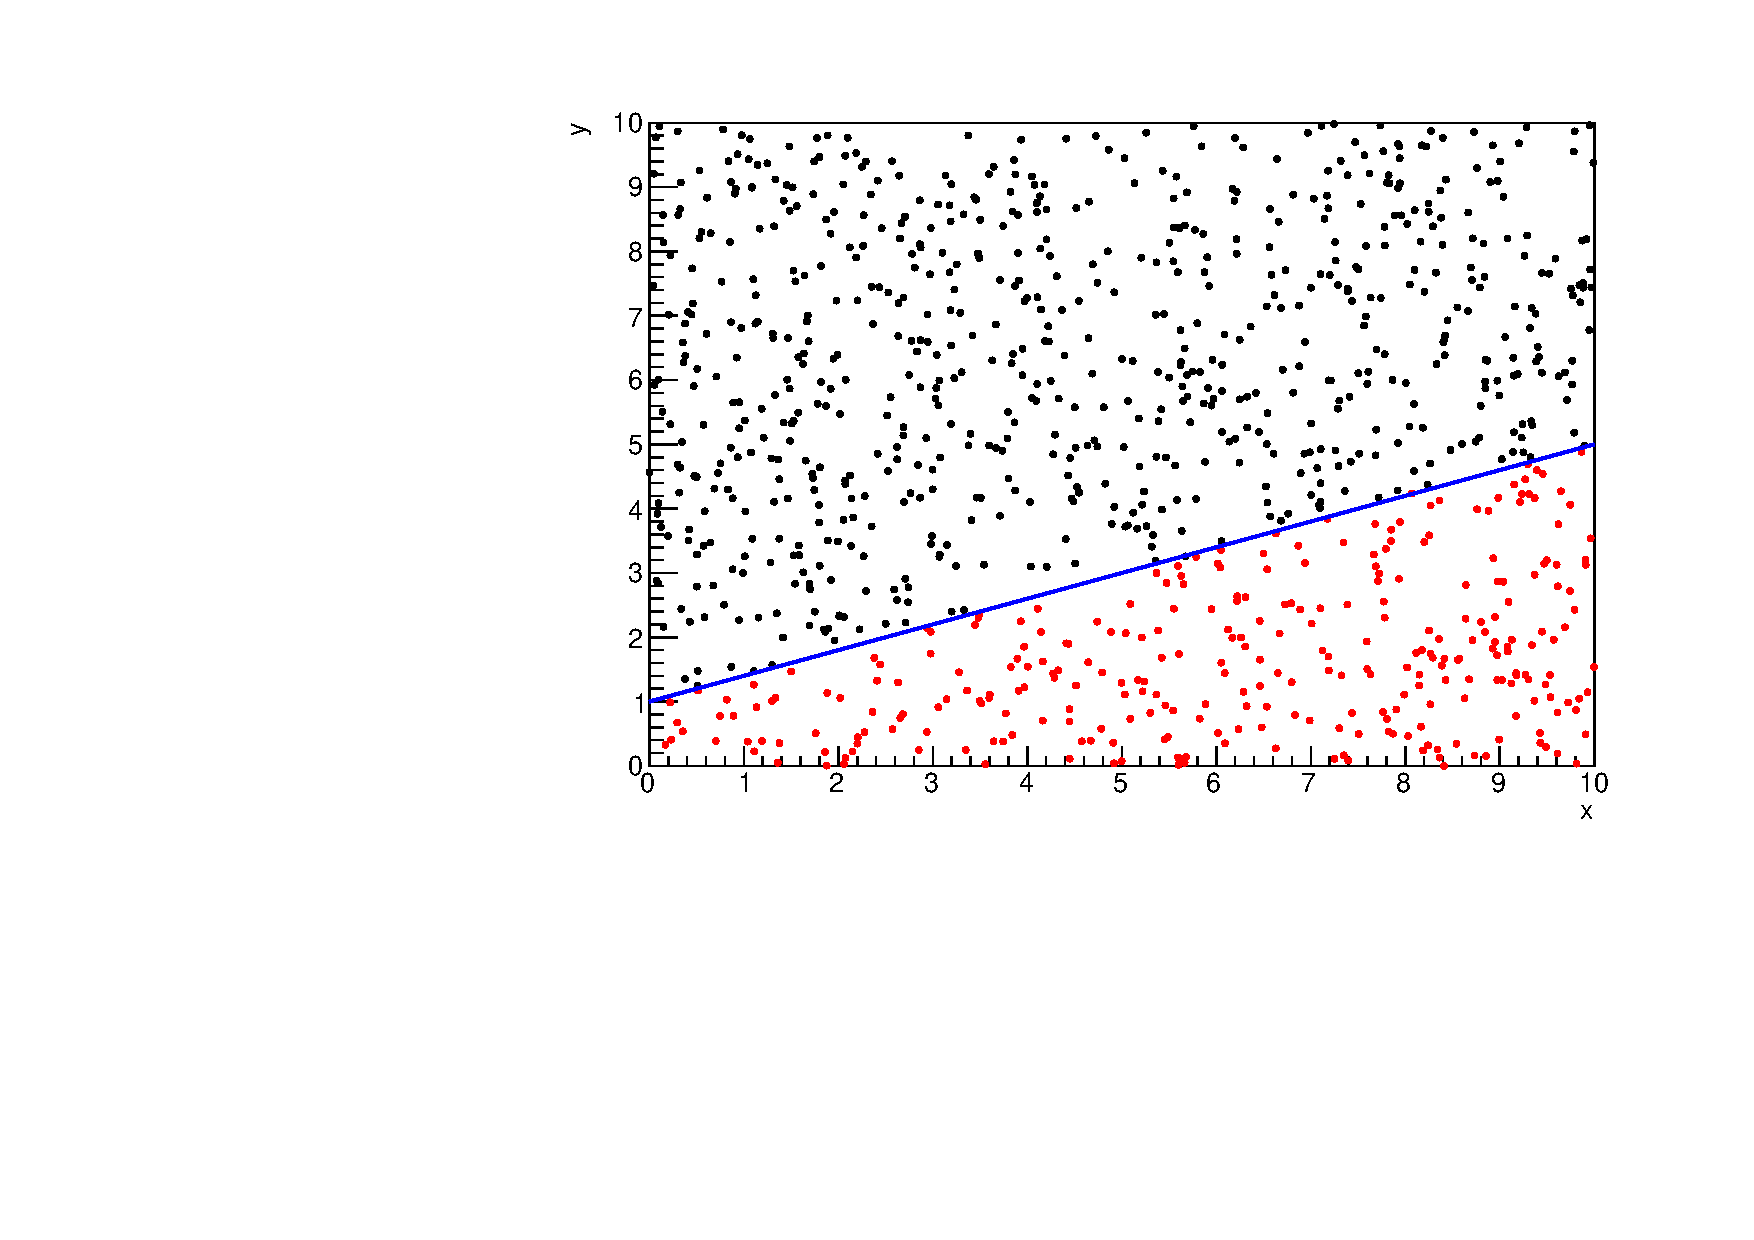
\includegraphics[width=\textwidth, trim={0mm 0mm 0mm 0mm}, clip,page=1]{Figures/MCMC/MCTechnique.pdf}
  \end{subfigure}
  \caption{Example of using Monte Carlo techniques to find the area under the blue line. The gradient and intercept of the line are \quickmath{0.4} and \quickmath{1.0} respectively. The area found to be under the curve using one thousand samples is \quickmath{29.9} units.}
  \label{fig:MCMC_MCTechnique}
\end{figure}

\begin{figure}[h]
  \begin{subfigure}[t]{0.80\textwidth}
    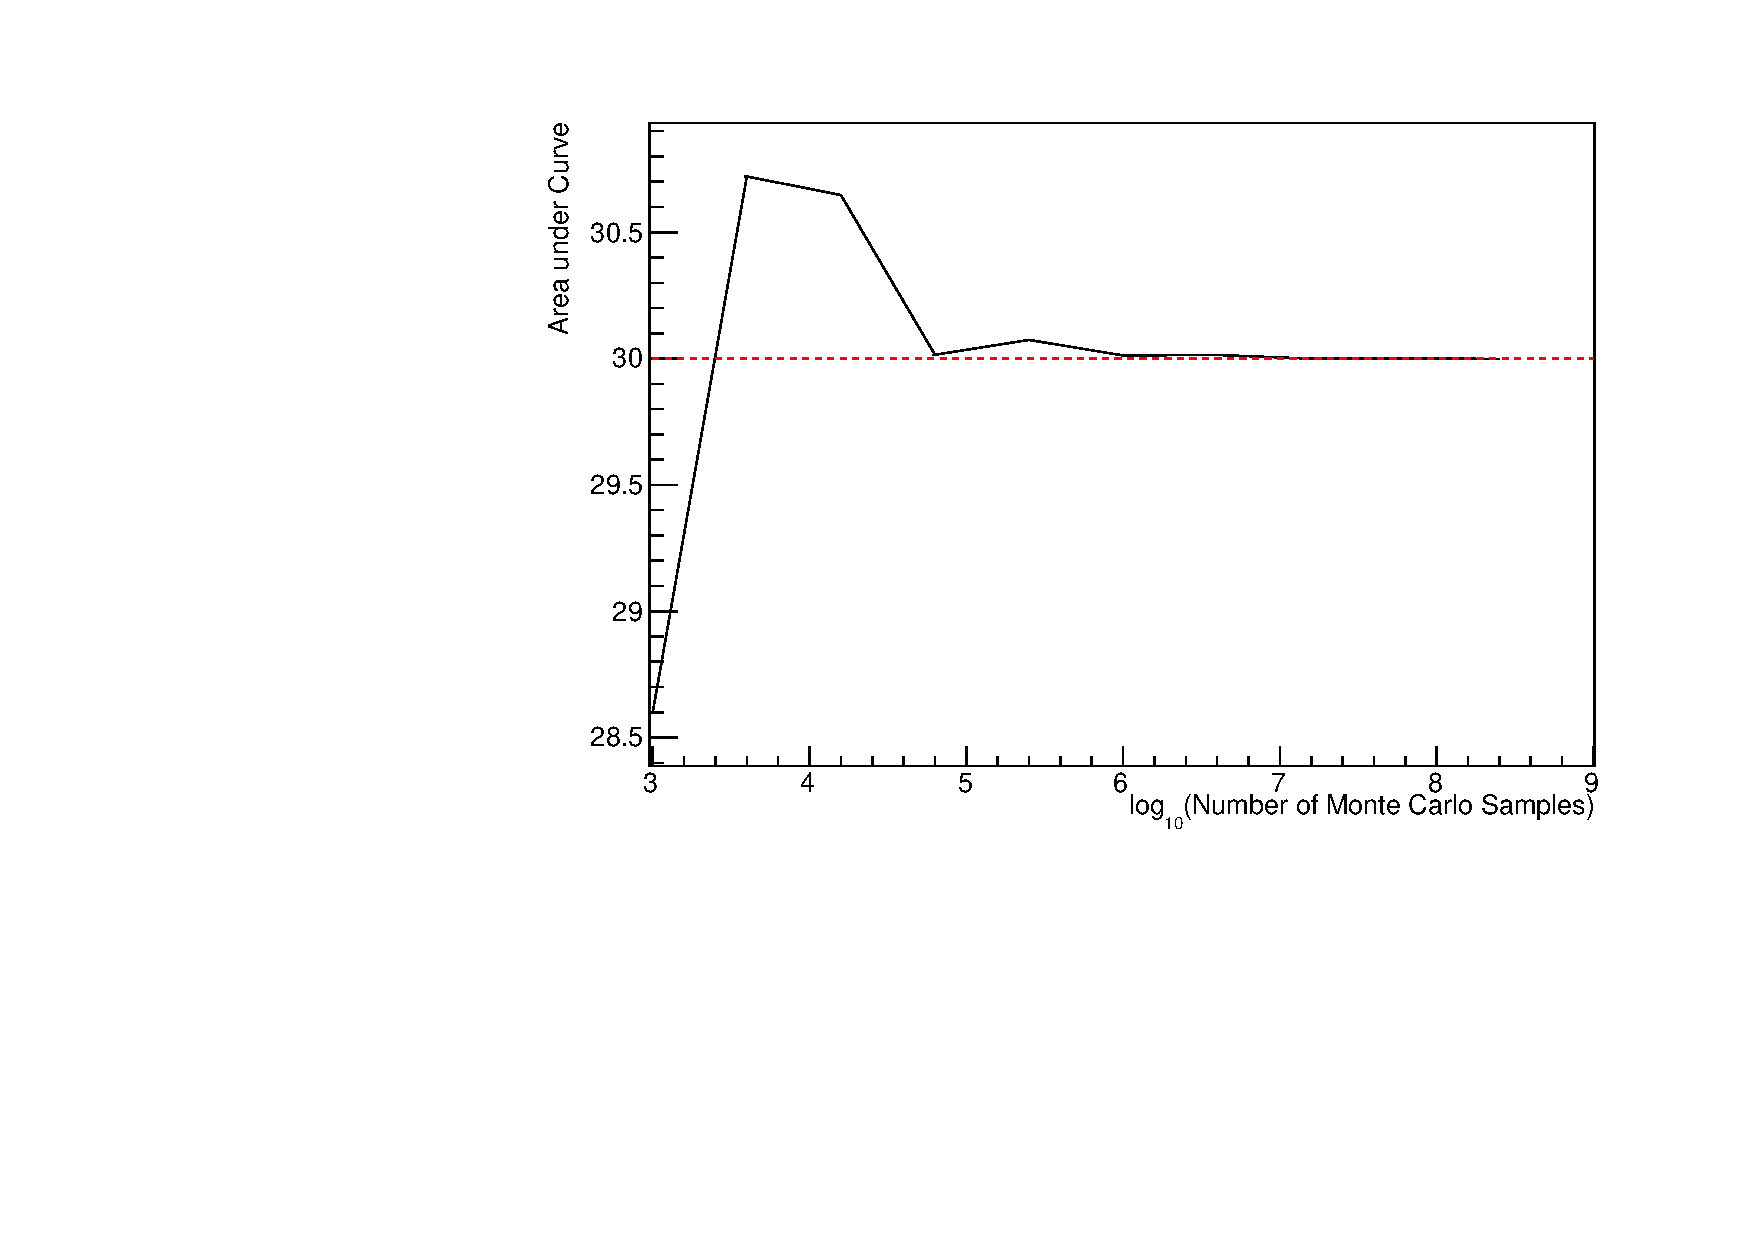
\includegraphics[width=\textwidth, trim={0mm 0mm 0mm 0mm}, clip,page=1]{Figures/MCMC/MCTechnique_NThrowsStudy.pdf}
  \end{subfigure}
  \caption{The area under a line of gradient \quickmath{0.4} and intercept \quickmath{1.0} for the range \quickmath{0 \leq x \leq 10} as calculated using Monte Carlo techniques as a function of the number of samples used in each repetition. The analytical solution to the area is 30 units as given by the red line.}
  \label{fig:MCMC_MCTechniqueNThrowsStudy}
\end{figure}

\subsection{Markov Chain Monte Carlo}
\label{sec:MarkovChainMonteCarlo_MarkovChainMC}
This analysis utilises a multi-dimensional probability distribution, with some dimensions being significantly more constrained than others. These constraints can be from prior knowledge of parameter distributions from external data or un-physical regions in which parameters can not exist. To maximise the efficiency of building the posterior distribution, a Markov Chain Monte Carlo (MCMC) technique is used. This employs a Markov chain to select the points at which to sample the posterior distribution. It performs a semi-random stochastic walk through the allowable parameter space. This builds a posterior distribution which has the property that the density of sampled points is proportional to the probability density of that parameter. This means that the samples produced by this technique are not statistically independent but they will cover the space of the distribution.

A Markov chain functions by selecting the position of step \quickmath{\vec{x}_{i+1}} based on the position of \quickmath{\vec{x}_{i}}. The space in which the Markov chain selects samples is dependent upon the total number of parameters utilised within the fit, where a discrete point in this space is described by the N-dimensional space \quickmath{\vec{x}}. In a perfectly operating Markov chain, the position of the next step depends solely on the previous step and not on the further history of the chain (\quickmath{\vec{x}_{0}}, \quickmath{\vec{x}_{1}}, etc.). However, in solving the multi-dimensionality of the fit used within this analysis, each step becomes correlated with several of the steps preceding itself.
%This behaviour is further explained in \autoref{sec:MarkovChainMonteCarlo_MCMCOptimisation}.
Providing the MCMC chain is well optimised, it will begin to converge towards a unique stationary distribution. The period between the chain's initial starting point and the convergence to the unique stationary distribution is colloquially known as the burn-in period.
%This is discussed further in \autoref{sec:MarkovChainMonteCarlo_MCMCOptimisation}.
Once the chain reaches the stationary distribution, all points sampled after that point will look like samples from that distribution.

Further details of the theories underpinning MCMC techniques are discussed in \cite{mcmc_practice} but can be summarised by the requirement that the chain satisfies the three `regularity conditions':

\begin{itemize}
\item Irreducibility: From every position in the parameter space \quickmath{\vec{x}}, there must exist a non-zero probability for every other position in the parameter space to be reached.
\item Recurrence: Once the chain arrives at the stationary distribution, every step following from that position must be samples from the same stationary distribution.
\item Aperiodicity: The chain must not repeat the same sequence of steps at any point throughout the sampling period.
\end{itemize}

The output of the chain after burn-in (i.e. the sampled points after the chain has reached the stationary distribution) can be used to approximate the posterior distribution and model parameters \quickmath{\vec{\theta}}. To achieve the requirement that the unique stationary distribution found by the chain be the posterior distribution, one can use the Metropolis-Hastings algorithm. This guides the stochastic process depending on the likelihood of the current proposed step compared to that of the previous step. %Implementation and other details of this technique are discussed in \autoref{sec:MarkovChainMonteCarlo_MetropoliseHastingsAlgorithm}.

\subsection{Metropolis-Hastings Algorithm}
\label{sec:MarkovChainMonteCarlo_MetropoliseHastingsAlgorithm}

As a requirement for MCMCs, the Markov chain implemented in this technique must have a unique stationary distribution that is equivalent to the posterior distribution. To ensure this requirement and that the regularity conditions are met, this analysis utilises the Metropolis-Hastings (MH) algorithm \cite{metropolis, hastings}. For the \quickmath{i^{th}} step in the chain, the MH algorithm determines the position in the parameter space to which the chain moves to based on the current step, \quickmath{\vec{x}_{i}}, and the proposed step, \quickmath{\vec{y}_{i+1}}. The proposed step is randomly selected from some proposal function \quickmath{f(\vec{x}_{i+1}|\vec{x}_{i})}, which depends solely on the current step (ie. not the further history of the chain). The next step in the chain \quickmath{\vec{x}_{i+1}} can be either the current step or the proposed step determined by whether the proposed step is accepted or rejected. To decide if the proposed step is selected, the acceptance probability, \quickmath{\alpha(\vec{x}_{i},\vec{y}_{i})}, is calculated as

\begin{equation}
  \label{eq:MarkovChainMonteCarlo_FullAcceptanceProbability}
  \alpha(\vec{x}_{i},\vec{y}_{i+1}) = \min\left(1,\frac{P(\vec{y}_{i+1}|D)f(\vec{x}_{i}|\vec{y}_{i+1})}{P(\vec{x}_{i}|D)f(\vec{y}_{i+1}|\vec{x}_{i})} \right).
\end{equation}

Where \quickmath{P(\vec{y}_{i+1}|D)} is the posterior distribution as introduced in \autoref{sec:MarkovChainMonteCarlo_BayesianStatistics}. To simplify this calculation, the proposal function is required to be symmetric such that \quickmath{f(\vec{x}_{i}|\vec{y}_{i+1}) = f(\vec{y}_{i+1}|\vec{x}_{i})}. In practice, a multi-variate Gaussian distribution is used to throw parameter proposals. This reduces \autoref{eq:MarkovChainMonteCarlo_FullAcceptanceProbability} to

\begin{equation}
  \label{eq:MarkovChainMonteCarlo_ReducedAcceptanceProbability}
  \alpha(\vec{x}_{i},\vec{y}_{i+1}) = \min\left(1,\frac{P(\vec{y}_{i+1}|D)}{P(\vec{x}_{i}|D)} \right).
\end{equation}

\finish{Figure out what Giles means}

After calculating this quantity, a random number, \quickmath{\beta}, is generated uniformly between 0 and 1. If \quickmath{\beta \leq \alpha(\vec{x}_{i},\vec{y}_{i+1})}, the proposed step is accepted. Otherwise, the chain sets the next step equal to the current step. This procedure is repeated for subsequent steps. This can be interpreted as if the posterior probability of the proposed step is greater than that of the current step, (\quickmath{P(\vec{y}_{i+1}|D) \geq P(\vec{x}_{i}|D)}), the proposed step will always be accepted. If the opposite is true, (\quickmath{P(\vec{y}_{i+1}|D) \leq P(\vec{x}_{i}|D)}), the proposed step will be accepted with probability \quickmath{P(\vec{x}_{i}|D) / P(\vec{y}_{i+1}|D)}. This ensures that the Markov chain does not get trapped in any local minima in the potentially non-Gaussian posterior distribution. The outcome of this technique is that the density of steps taken in a discrete region is directly proportional to the probability density in that region.

\subsection{MCMC Optimisation}
\label{sec:MarkovChainMonteCarlo_MCMCOptimisation}
As discussed in \autoref{sec:MarkovChainMonteCarlo_MetropoliseHastingsAlgorithm}, the proposal function invoked within the MH algorithm can take any form and the chain will still converge to the stationary distribution. At each set of proposed parameter values, a prediction of the same spectra has to be generated which requires significant computational resources. Therefore, the number of steps taken before the unique stationary distribution is found should be minimised as only steps after convergence add information to the oscillation analysis. Furthermore, the chain should entirely cover the allowable parameter space to ensure that all values have been considered. Tuning the distance that the proposal function jumps between steps on a parameter-by-parameter basis can both minimise the length of the burn-in period and ensure that the correlation between step \quickmath{\vec{x}_{i}} and \quickmath{\vec{x}_{j}} is sufficiently small.

The effect of changing the width of the proposal function is highlighted in \autoref{fig:MCMC_MCTechniqueStepSizeStudy}. Three scenarios, each with the same underlying stationary distribution (A Gaussian of width \quickmath{1.0} and mean \quickmath{0.}), are presented. The only difference between the three scenarios is the width of the proposal function, colloquially known as the `step size \quickmath{\sigma}'. Each scenario starts at an initial parameter value of \quickmath{10.0} which would be considered an extreme variation. For the case where \quickmath{\sigma = 0.1}, it is clear to see that the chain takes a long time to reach the expected region of the parameter. This indicates that this chain would have a large burn-in period and does not converge to the stationary distribution until step \quickmath{\sim 500}. Furthermore, whilst the chain does move towards the expected region, each step is significantly correlated with the previous. Considering the case where \quickmath{\sigma = 5.0}, the chain approaches the expected parameter region almost instantly meaning that the burn-in period is not significant. However, there are clearly large regions of steps where the chain does not move. This is likely due to the chain proposing steps in the tails of the distribution which have a low probability of being accepted. Consequently, this chain would take a significant number of steps to fully span the allowable parameter region. For the final scenario, where \quickmath{\sigma = 0.5}, you can see a relatively small burn-in period of approximately \quickmath{100} steps. Once the chain reaches the stationary distribution, it moves throughout the expected region of parameter values many times, sufficiently sampling the full parameter region. This example is a single parameter varying across a continuous distribution and does not fully reflect the difficulties in the many-hundred multi-variate parameter distribution used within this analysis. However, it does give a conceptual idea of the importance of selecting the proposal function and associated step size. 

\begin{figure}[h]
  \begin{subfigure}[t]{\textwidth}
    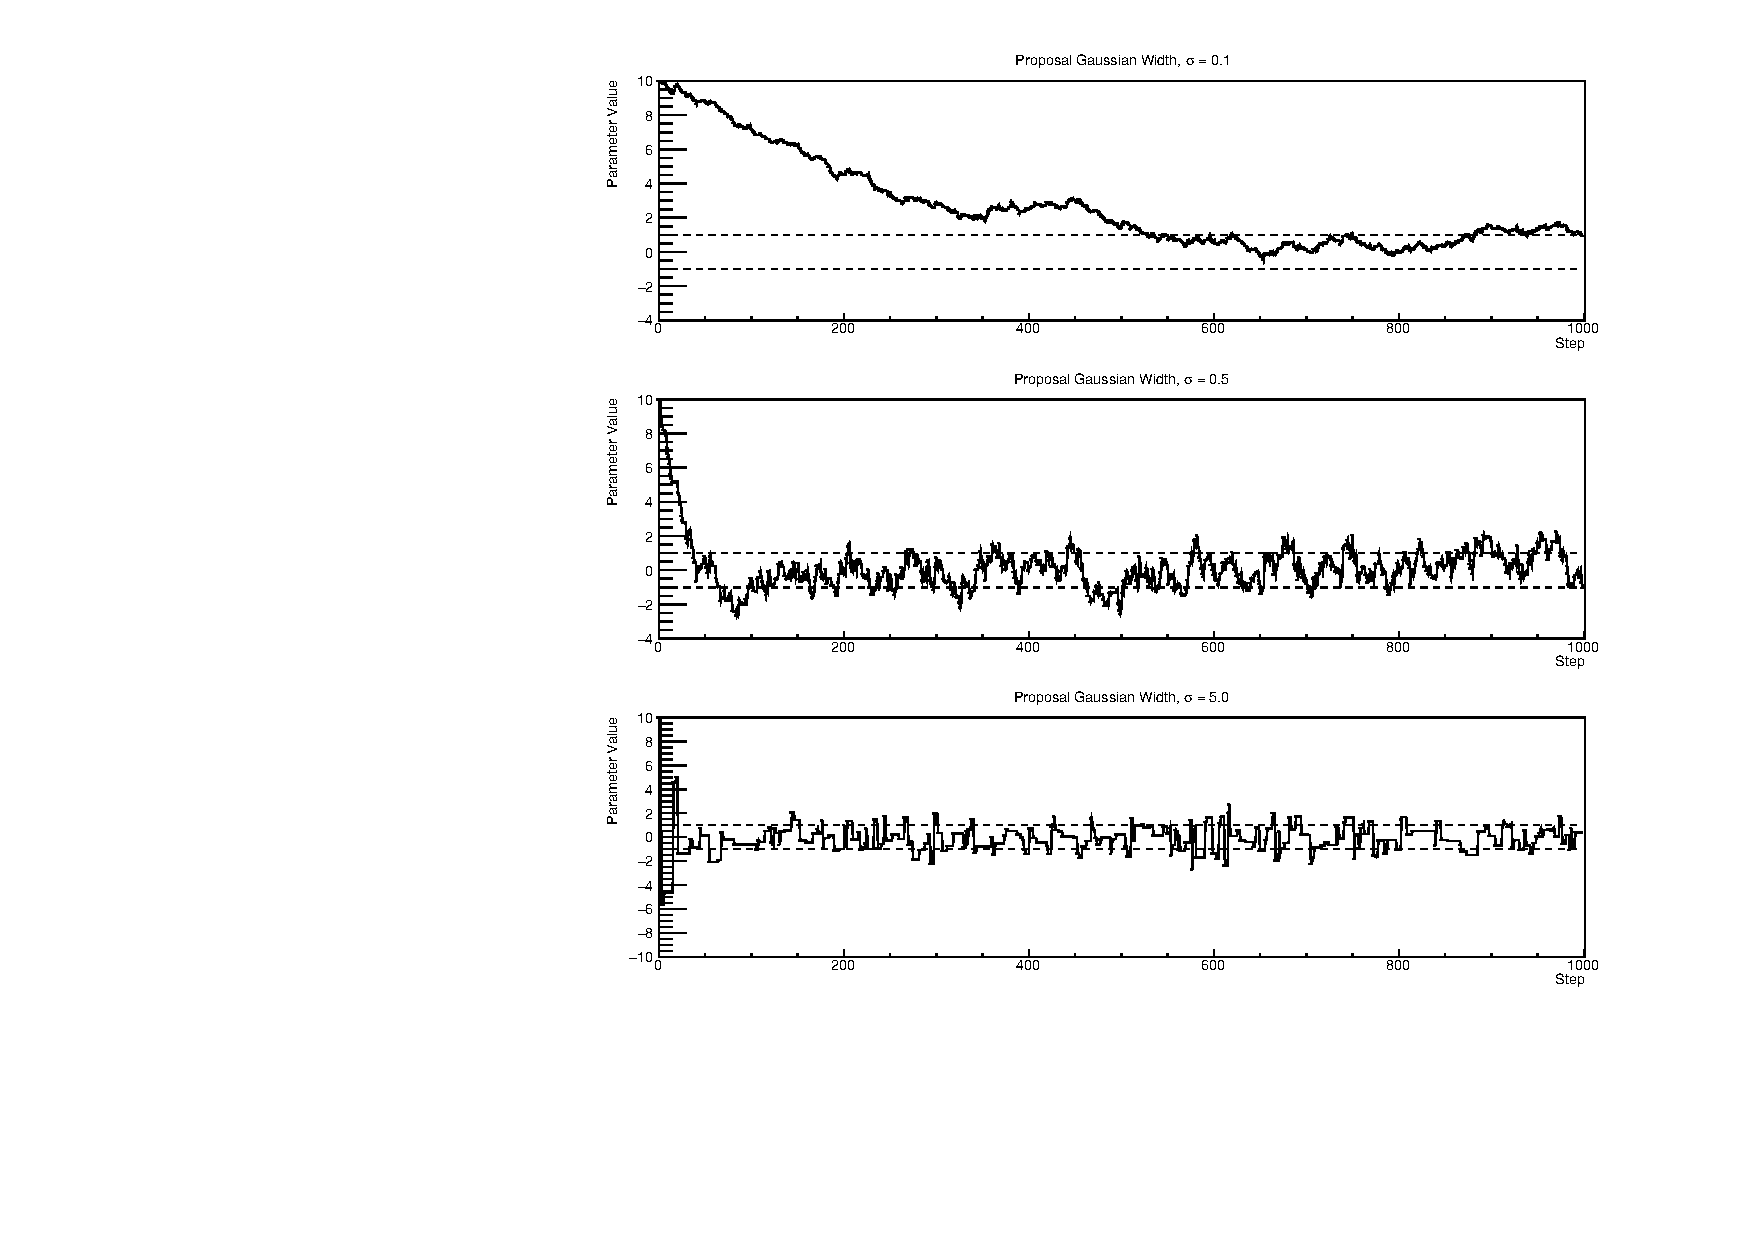
\includegraphics[width=\textwidth, trim={10mm 0mm 18mm 0mm}, clip,page=1]{Figures/MCMC/MCMCTechnique_StepSizes.pdf}
  \end{subfigure}
  \caption{Three MCMC chains, each with a stationary distribution equal to a Gaussian centered at \quickmath{0} and width \quickmath{1} (As indicated by the black dotted lines). All of the chains use a Gaussian proposal function but have different widths (or `step size \quickmath{\sigma}'). The top panel has \quickmath{\sigma = 0.1}, middle panel has \quickmath{\sigma = 0.5} and the bottom panel has \quickmath{\sigma = 5.0}.}
  \label{fig:MCMC_MCTechniqueStepSizeStudy}
\end{figure}

As discussed, step size tuning directly correlates to the average step acceptance rate. If the step size is too small, many steps will be accepted but the chain moves slowly. If the opposite is true, many steps will be rejected as the chain proposes steps in the tails of the distribution. Discussion in \cite{Dunkley2005-xz} suggests that the `ideal' acceptance rate of a high dimension MCMC chain should be approximately \quickmath{\sim 25\%}. An ``ideal'' step size \cite{Dunkley2005-xz} of

\begin{equation}
  \label{eq:MCMC_IdealStepSize}
  \sigma = \frac{2.4}{N_{p}},
\end{equation}

where \quickmath{N_{p}} is the number of parameters included in the MCMC fit. However, the complex correlations between systematics mean that some parameters have to be hand-tuned and many efforts have been taken to select a set of parameter-by-parameter step sizes to approximately reach the ideal acceptance rate.

\autoref{fig:MCMC_MCTechniqueLLHVsStep} highlights the likelihood as calculated by the fit in \finish{Link to AsimovA Sensitivity Section} as a function of the number of steps in each chain. In practice, many independent MCMC chains are run simultaneously to parallelise the task of performing the fit. This figure overlays the distribution found in each chain. As seen, the likelihood decreases from its initial value and converges towards a stationary distribution after \quickmath{\sim 1 \times 10^{5}} steps.

\begin{figure}[h]
  \begin{subfigure}[t]{0.8\textwidth}
    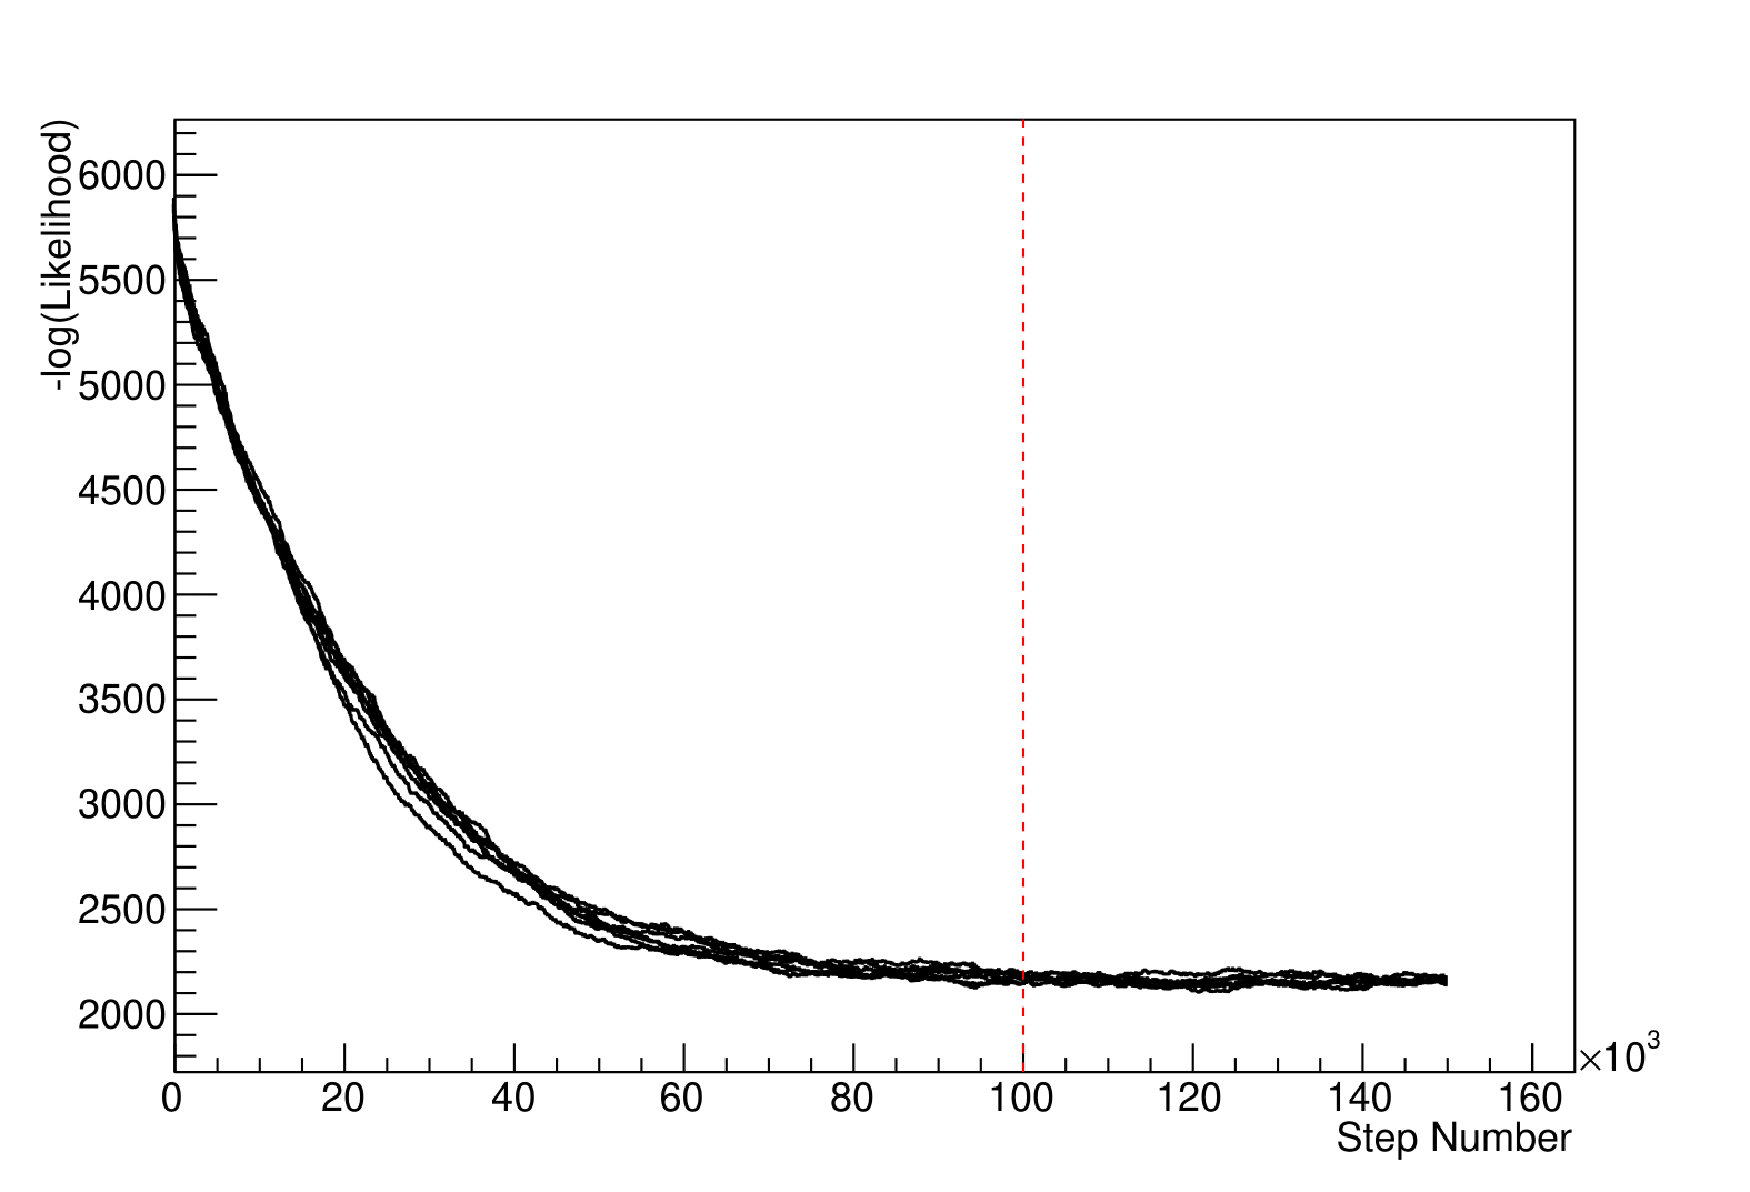
\includegraphics[width=\textwidth, trim={0mm 0mm 0mm 0mm}, clip,page=1]{Figures/MCMC/MCTechnique_LLHStep.pdf}
  \end{subfigure}
  \caption{The log-likelihood from the fit detailed in \finish{Link to AsimovA Sensitivity Section} as a function of the number of steps accumulated in each fit. Many independent MCMC chains were run in parallel and overlaid on this plot. The red line indicates the \quickmath{1 \times 10^{5}} step burn-in period after which the log-likelihood becomes stable.}
  \label{fig:MCMC_MCTechniqueLLHVsStep}
\end{figure}

Multiple configurations of this analysis have been performed throughout this thesis where different samples or systematics have been used. For all of these configurations, it was found that a burnin period of \quickmath{1 \times 10^{5}} was sufficient in all cases.

\section{Understanding the MCMC Results}
\label{sec:MarkovChainMonteCarlo_UnderstandingMCMCResults}

The previous sections have described how to generate the posterior probability distribution using Bayesian MCMC techniques. However, this analysis focuses on oscillation parameter determination. The posterior distribution output from the chain is a high-dimension object, with as many dimensions as there are parameters included in the oscillation analysis. However, this multi-dimensional object is difficult to conceptualize so parameter estimations are often presented in one or two-dimensional projections of this probability distribution. To do this, we invoke the marginalisation technique highlighted in \autoref{sec:MarkovChainMonteCarlo_Marginalisation}.

\subsection{Marginalisation}
\label{sec:MarkovChainMonteCarlo_Marginalisation}

The output of the MCMC chain is a highly dimensional probability distribution which is very difficult to interpret. From the standpoint of an oscillation analysis experiment, the one or two-dimensional `projections' of the oscillation parameters of interest are most relevant. Despite this, the best fit values and uncertainties on the oscillation parameters of interest should correctly encapsulate the correlations to the other systematic uncertainties (colloquially called `nuisance' parameters). For this joint beam and atmospheric analysis, the oscillation parameters of interest are \quickmath{\sin^{2}(\theta_{23})}, \quickmath{\sin^{2}(\theta_{13})}, \quickmath{\Delta m^{2}_{32}}, and\quickmath{\delta_{CP}}. All other parameters (including the oscillation parameters this fit is insensitive to) are deemed nuisance parameters. To generate these projections, we rely upon integrating the posterior distribution over all nuisance parameters. This is called marginalisation. This technique also explains why it is acceptable to neglect the normalisation constant of the posterior distribution, which was discussed in \autoref{sec:MarkovChainMonteCarlo_BayesianStatistics}.

A simple example of the marginalisation technique is to imagine the scenario where two coins are flipped. To determine the probability that the first coin returned a `head', the exact result of the second coin flip is disregarded and simply integrated over. For the parameters of interest, \quickmath{\vec{\theta}_{i}}, we can calculate the marginalised posterior by integrating over the nuisance parameters, \quickmath{\vec{\theta}_{n}}. In this case, \autoref{eq:MarkovChainMonteCarlo_PosteriorDistribution} becomes

\begin{equation}
P(\vec{\theta}_{i}|D) = \frac{\int P(D|\vec{\theta}_{i},\vec{\theta}_{n}) P(\vec{\theta}_{i},\vec{\theta}_{n}) d\vec{\theta}_{n}}{\int P(D|\vec{\theta}) P(\vec{\theta}) d\vec{\theta}}
\end{equation}

Where \quickmath{P(\vec{\theta}_{i},\vec{\theta}_{n})} encodes the prior knowledge about the uncertainty and correlations between the parameters of interest and the nuisance parameters. In practice, this is simply taking the one or two-dimensional projection of the multi-dimensional probability distribution.

While in principle an easy solution to a complex problem, correlations between the interesting and nuisance parameters can bias the marginalised results. A similar effect is found when the parameters being marginalised over have non-Gaussian probability distributions. For example, \autoref{fig:MCMC_MCTechniqueMarginalisationProblems} highlights the marginalisation bias in the probability distribution found for a parameter when requiring a correlated parameter to have a positive parameter value. Due to the complex nature of the oscillation parameter fit presented in this thesis, there are correlations occurring between the oscillation parameters of interest and the other nuisance parameters included in the fit.

\begin{figure}[h]
  \begin{subfigure}[t]{0.48\textwidth}
    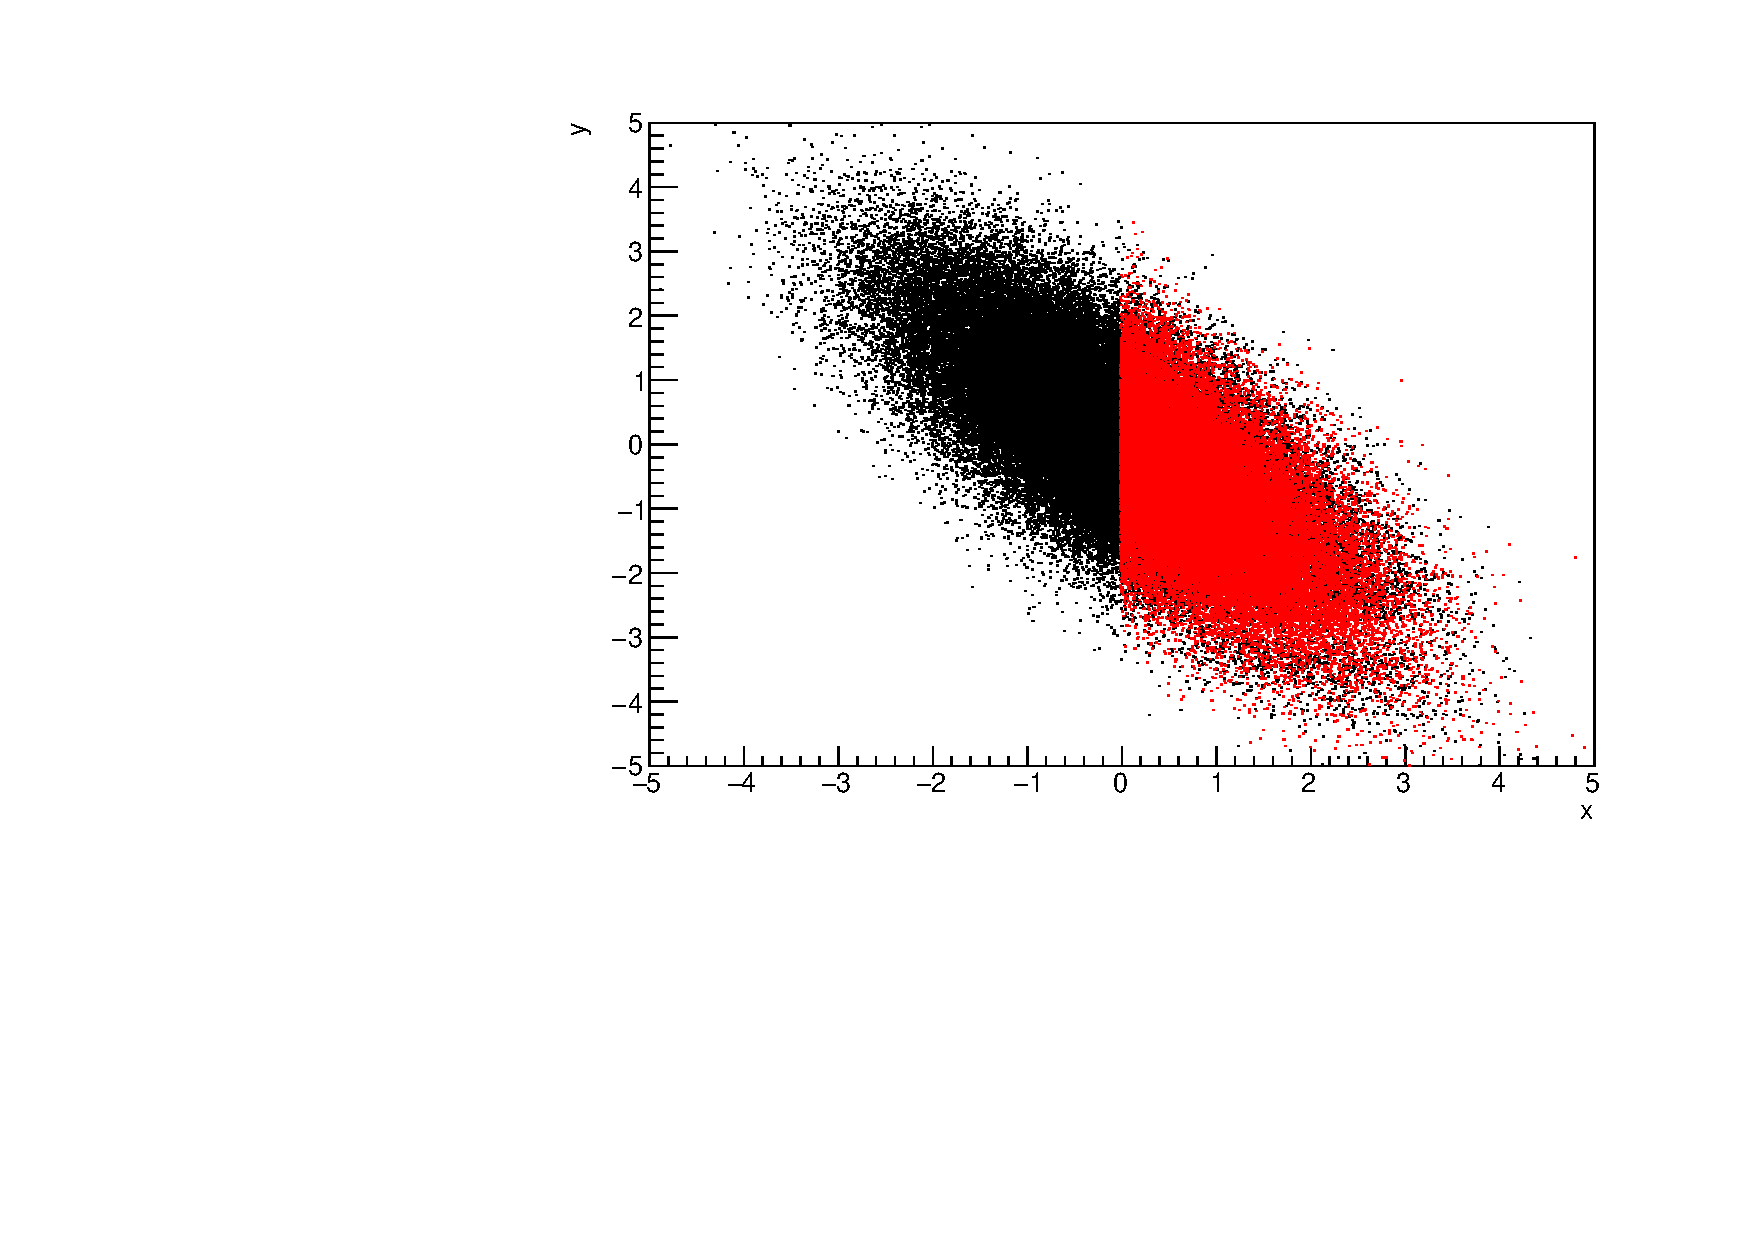
\includegraphics[width=\textwidth, trim={0mm 0mm 0mm 0mm}, clip,page=1]{Figures/MCMC/MCTechnique_Marginalisation2D_Double_Correlations.pdf}
  \end{subfigure} %
    \begin{subfigure}[t]{0.48\textwidth}
    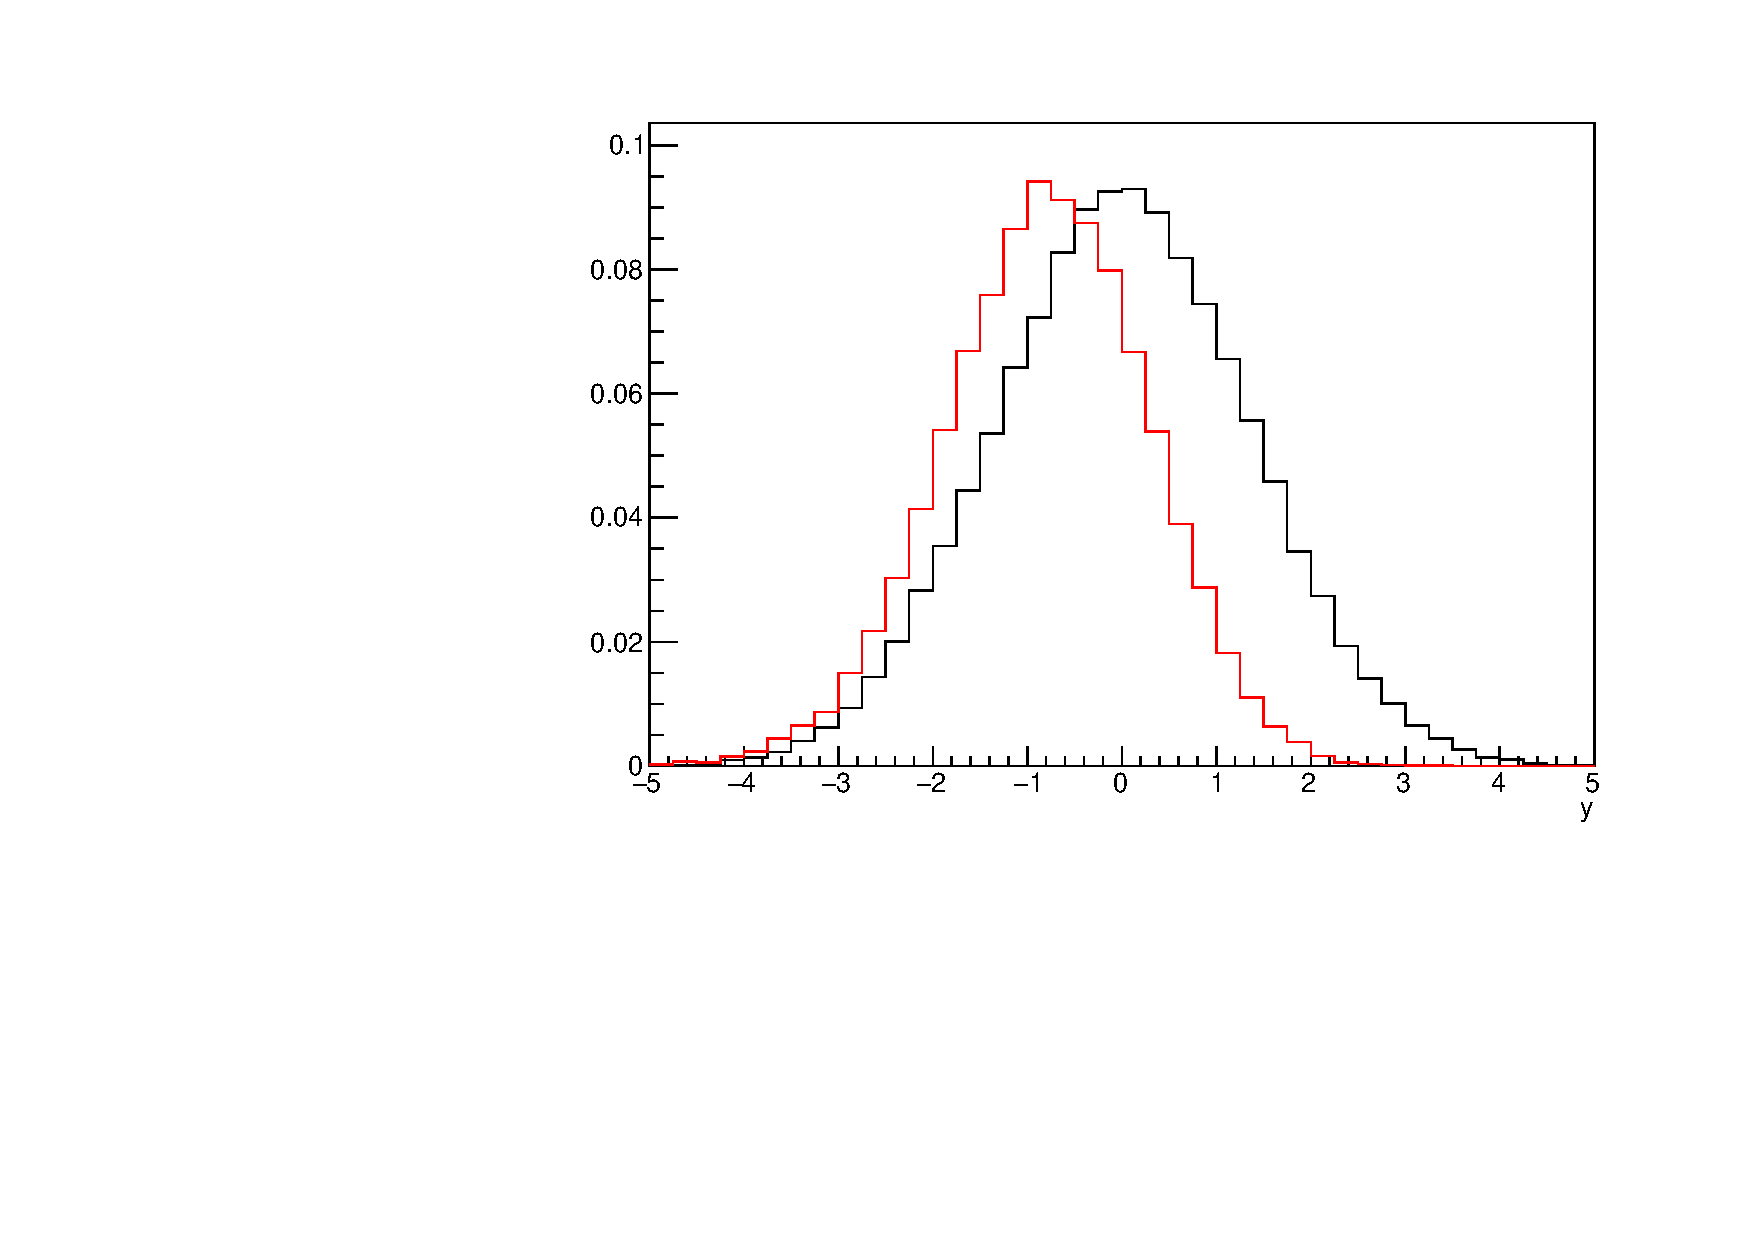
\includegraphics[width=\textwidth, trim={0mm 0mm 0mm 0mm}, clip,page=1]{Figures/MCMC/MCTechnique_Marginalisation1D_Double_Correlations.pdf}
  \end{subfigure}

  \caption{Left: The two-dimensional probability distribution for two correlated parameters \quickmath{x} and \quickmath{y}. The red distribution shows the two-dimensional probability distribution when \quickmath{0 \leq x \leq 5}. Right: The marginalised probability distribution for the \quickmath{y} parameter found when requiring the \quickmath{x} to be bound between \quickmath{-5 \leq x \leq 5} and \quickmath{0 \leq x \leq 5} for the black and red distribution, respectively.}
  \label{fig:MCMC_MCTechniqueMarginalisationProblems}
\end{figure}

\subsection{Parameter Estimation and Credible Intervals}
\label{sec:MarkovChainMonteCarlo_ParameterEstimation}

The purpose of this analysis is to determine the best fit values for the oscillation parameters that the beam and atmospheric samples are sensitive to: \quickmath{\sin^{2}(\theta_{23})}, \quickmath{\sin^{2}(\theta_{13})}, \quickmath{\Delta m^{2}_{32}}, and \quickmath{\delta_{CP}}.
%Typically, the results presented take the form of one or two-dimension marginalised probability distributions for the appearance (\quickmath{\sin^{2}(\theta_{13})} and \quickmath{\delta_{CP}}) and disappearance (\quickmath{\sin^{2}(\theta_{23})} and \quickmath{\Delta m^{2}_{32}}) parameters.
The posterior probability density, taken from the output MCMC chain, is binned in these parameters. The parameter best-fit point is then taken to be the value that has the highest posterior probability. This is performed in both one and two-dimensional projections.

However, the single best-fit point in a given parameter is not of much use on its own. We would also like to determine the uncertainty, or credible interval, on that best-fit point. The definition of the \quickmath{1\sigma} credible interval is that we have \quickmath{68\%} belief that the parameter is within those bounds. For a more generalised definition, the credible interval is the region, \quickmath{R}, of the posterior distribution that contains a specific fraction of the total probability, such that

\begin{equation}
\int_{R} P(\theta|D)d\theta = \alpha
\end{equation}

Where \quickmath{\theta} is the parameter on which we calculate the credible interval. This technique then calculates the \quickmath{\alpha \times 100\%} credible interval.

In practice, this analysis uses the highest posterior density (HPD) credible intervals which are calculated through the following method. First, the probability distribution is area-normalised such that it has an integrated area equal to \quickmath{1.0}. The bins of probability are then summed from the highest to lowest until the sum exceeds the \quickmath{1\sigma} level (\quickmath{0.68} in this example). This process is repeated for a range of credible intervals, notably the \quickmath{1\sigma}, \quickmath{2\sigma} and \quickmath{3\sigma} along with other levels where the critical values for each level can be found in \cite{Particle_Data_Group2020-ms}. This process can be repeated for the two-dimensional probability distributions by creating two-dimensional contours of credible intervals rather than a one-dimensional result. 

\subsection{Bayesian Model Comparisons}
\label{sec:MarkovChainMonteCarlo_BayesTheorem}
Due to the matter resonance, this analysis has some sensitivity to the mass hierarchy of neutrino states (whether \quickmath{\Delta m^{2}_{32}} is positive or negative) and the octant of \quickmath{\sin^{2}(\theta_{23})}. The Bayesian approach utilised within this analysis gives an intuitive method of model comparison by determining which hypothesis is most favourable. Taking the ratio of \autoref{eq:MarkovChainMonteCarlo_PosteriorDistributionReduced} for the two hypotheses of normal hierarchy, \quickmath{NH}, and inverted hierarchy, \quickmath{IH}, gives

\begin{equation}
  \frac{P(\vec{\theta}_{NH}|D)}{P(\vec{\theta}_{IH}|D)} = \frac{P(D|\vec{\theta}_{NH})}{P(D|\vec{\theta}_{IH})} \times \frac{P(\vec{\theta}_{NH})}{P(\vec{\theta}_{IH})}.
\end{equation}

The middle term defines the Bayes factor, \quickmath{B(\text{NH}/\text{IH})}, which is a data-driven interpretation of how strong the data prefers one hierarchy to the other. For this analysis, equal priors on both mass hierarchy hypotheses are chosen (\quickmath{P(\vec{\theta}_{NH}) = P(\vec{\theta}_{IH})} = 0.5). In practice, the MCMC chain proposes a value of \quickmath{|\Delta m^{2}_{32}|} and then applies a \quickmath{50\%} probability that the value is sign flipped. Consequently, the Bayes factor can be calculated from the ratio of the probability density in either hypothesis. This equates to counting the number of steps taken in the normal and inverted hierarchies and taking the ratio. The same approach can be taken to compare the upper octant (UO) compared to the lower octant (LO) hypothesis of \quickmath{\sin^{2}(\theta_{23})}.

\begin{table}[ht!]
    \centering
    \begin{tabular}{c|c|l}
      \hline
      $\log_{10}(B_{AB})$ & $B_{AB}$ & Strength of Preference \\
      \hline
      \hline
      \quickmath{<0.0} & \quickmath{<1} & No preference for hypothesis A (Supports hypothesis B) \\
      \quickmath{0.0 - 0.5} & \quickmath{1.0 - 3.16} & Preference for hypothesis A is weak \\
      \quickmath{0.5 - 1.0} & \quickmath{3.16 - 10.0} & Preference for hypothesis A is substantial \\
      \quickmath{1.0 - 1.5} & \quickmath{10.0 - 31.6} & Preference for hypothesis A is strong \\
      \quickmath{1.5 - 2.0} & \quickmath{31.6 - 100.0} & Preference for hypothesis A is very strong \\
      \quickmath{>2.0 }& \quickmath{>100.0} & Decisive preference for hypothesis A \\
      \hline
      \hline
      
      \hline
    \end{tabular}
    \caption{Jeffreys scale for strength of preference for two models \quickmath{A} and \quickmath{B} as a function of the calculated Bayes factor (\quickmath{B_{AB} = B(A/B)}) between the two models \cite{Jeffreys:1939xee}. The original scale is given in terms of \quickmath{\log_{10}(B(A/B))} but converted to linear scale for easy comparison throughout this thesis.}
    \label{tab:MarkovChainMonteCarlo_JeffreysScale}
\end{table}

Whilst the value of the Bayes factor should always be shown, the Jeffreys scale \cite{Jeffreys:1939xee} (highlighted in \autoref{tab:MarkovChainMonteCarlo_JeffreysScale}) gives an indication of the strength of preference for one model compared to the other. Other interpretations of the strength of preference of a model exist, e.g. the Kass and Raferty Scale \cite{Kass1995-nl}.

\subsection{Comparison of MCMC Output to Expectation}
\label{sec:MarkovChainMonteCarlo_Predictives}

To ensure the fit is performing well, a best-fit spectrum is produced using the posterior probability distribution and compared with the data, allowing easy by-eye comparisons to be made. A simple method of doing this is to perform a comparison in the fitting parameters (For instance, the reconstructed neutrino energy and lepton direction for T2K far detector beam samples) of the spectra generated by the MCMC chain to `data'. This `data' could be true data or some variation of Monte Carlo prediction. This allows easy comparison of the MCMC probability distribution to the data. To perform this, \quickmath{N} steps from the post-burnin MCMC chain are randomly selected. From these, the Monte Carlo prediction at each step is generated by reweighting the model parameters to the values specified at that step. Due to the probability density being directly correlated with the density of steps in a certain region, parameter values close to the best fit value are most likely to be selected.

In practice, for each bin of the fitting parameters has a probability distribution of event rates, with one entry per sampled MCMC step. This distribution is binned where the bin with the highest probability is selected as the mean and an error on the width of this probability distribution is calculated using the approach highlighted in \autoref{sec:MarkovChainMonteCarlo_ParameterEstimation}. Consequently, the best fit distribution in the fit parameter is not necessarily that which would be attained by reweighting the Monte Carlo prediction to the most probable parameter values.

A similar study can be performed to illustrate the freedom of the model parameter space prior to the fit. This can be done by throwing parameter values from the prior uncertainty of each parameter.
%This becomes troublesome for parameters with no prior uncertainty as the range is technically infinite. Where applicable solutions to remove these have been addressed.

  \chapter{Simulation}
\label{chap:Simulation}
Simulation Chapter

\section{Beamline}
\label{sec:Simulation_Beamline}
Beamline Simulation Section

\section{Atmospheric Flux}
\label{sec:Simulation_AtmosphericFlux}
Atmospheric Flux Simulation Section

\section{Neutrino Interaction}
\label{sec:Simulation_NeutrinoInteraction}
Neutrino Interaction Simulation Section

\section{Near Detector}
\label{sec:Simulation_NearDetector}
Near Detector Simulation Section

\section{Far Detector}
\label{sec:Simulation_FarDetector}
Far Detector Section

\section{Event Reconstruction}
\label{sec:Simulation_EventReconstruction}
Event Reconstruction Section



  %\input{EventSelection}
  %\input{JointFit}
  %\input{Validation}
  %\input{DataFit}
  %\input{Conclusions}
\end{mainmatter}

%% Produce the appendices
\begin{appendices}
  \chapter{Atmospheric Sample Spectra}
\label{chap:AppendixA}

This appendix documents theinteraction mode breakdown of all the atmospheric samples used within the analysis. The generated tune of the model parameters and the Asimov A oscillation parameter set (defined in \autoref{tab:Theory_ParameterSets}) are assumed. The livetime of SK-IV is taken to be \quickmath{3244.4} days.

\section{Fully Contained Sub-GeV Samples}
The interaction mode breakdown of the fully contained Sub-GeV samples are shown in \autoref{fig:SKSamples:FCSubGeVCC0pi} and \autoref{fig:SKSamples:FCSubGeVCC1pi}, for the samples with enriched CC$0\pi$ and CC$1\pi^\pm$ respectively.

The CC$0\pi$ sample are dominated by CCQE events ($\sim 70\%$) with smaller contributions of 2p2h ($\sim 12\%$) and CC$1\pi$ ($\sim 10\%$) components. The energy peaks around $300$~MeV, which is slightly below that of the T2K samples but still has significant contribution upto $1$~GeV which overlaps the T2K sample energy range.

The one-ring CC$1\pi$ samples, where the pion is tagged via its decay electron, are dominated by CC$1\pi$ events ($\sim 75\%$) with a small contribution of CC$M\pi$ ($\sim 10\%$). The two-ring pion sample is mostly dominated by the NC$1\pi^0$ via resonances, and has several equally-sized contributions from CCQE, NC$1\pi^\pm$ via resonances, and NC coherent pion production, where the $\pi^0$ likely comes from nucleon and $\pi^\pm$ final state interactions in the nucleus.

\begin{figure}[ht]
    \begin{subfigure}[t]{0.49\textwidth}
    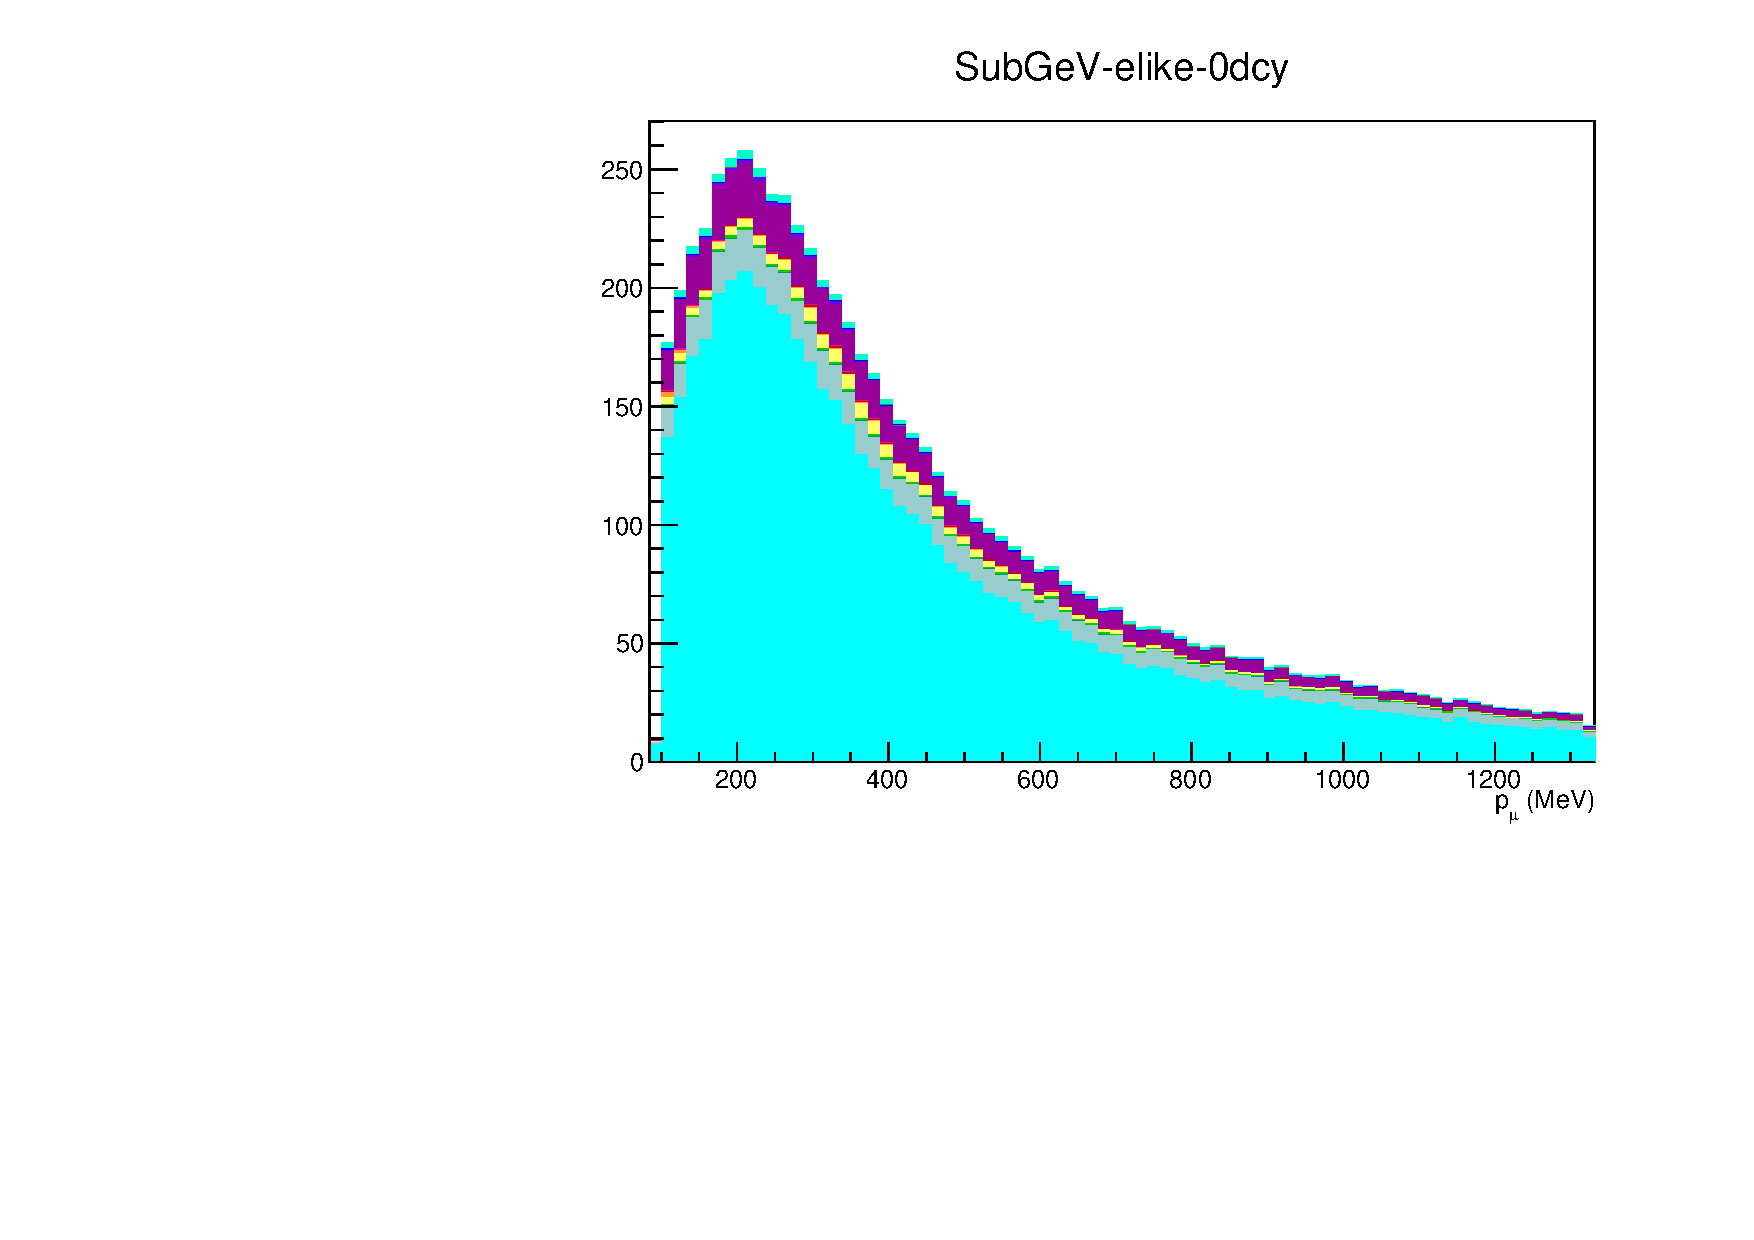
\includegraphics[width=\textwidth, trim= 0 0 0 30, clip]{Figures/Selections/AtmosphericByMode/SubGeV-elike-0dcy_LepMom.pdf}
    \caption{FC Sub-GeV 1R e-like 0 de}
    \end{subfigure}
    \begin{subfigure}[t]{0.49\textwidth}
    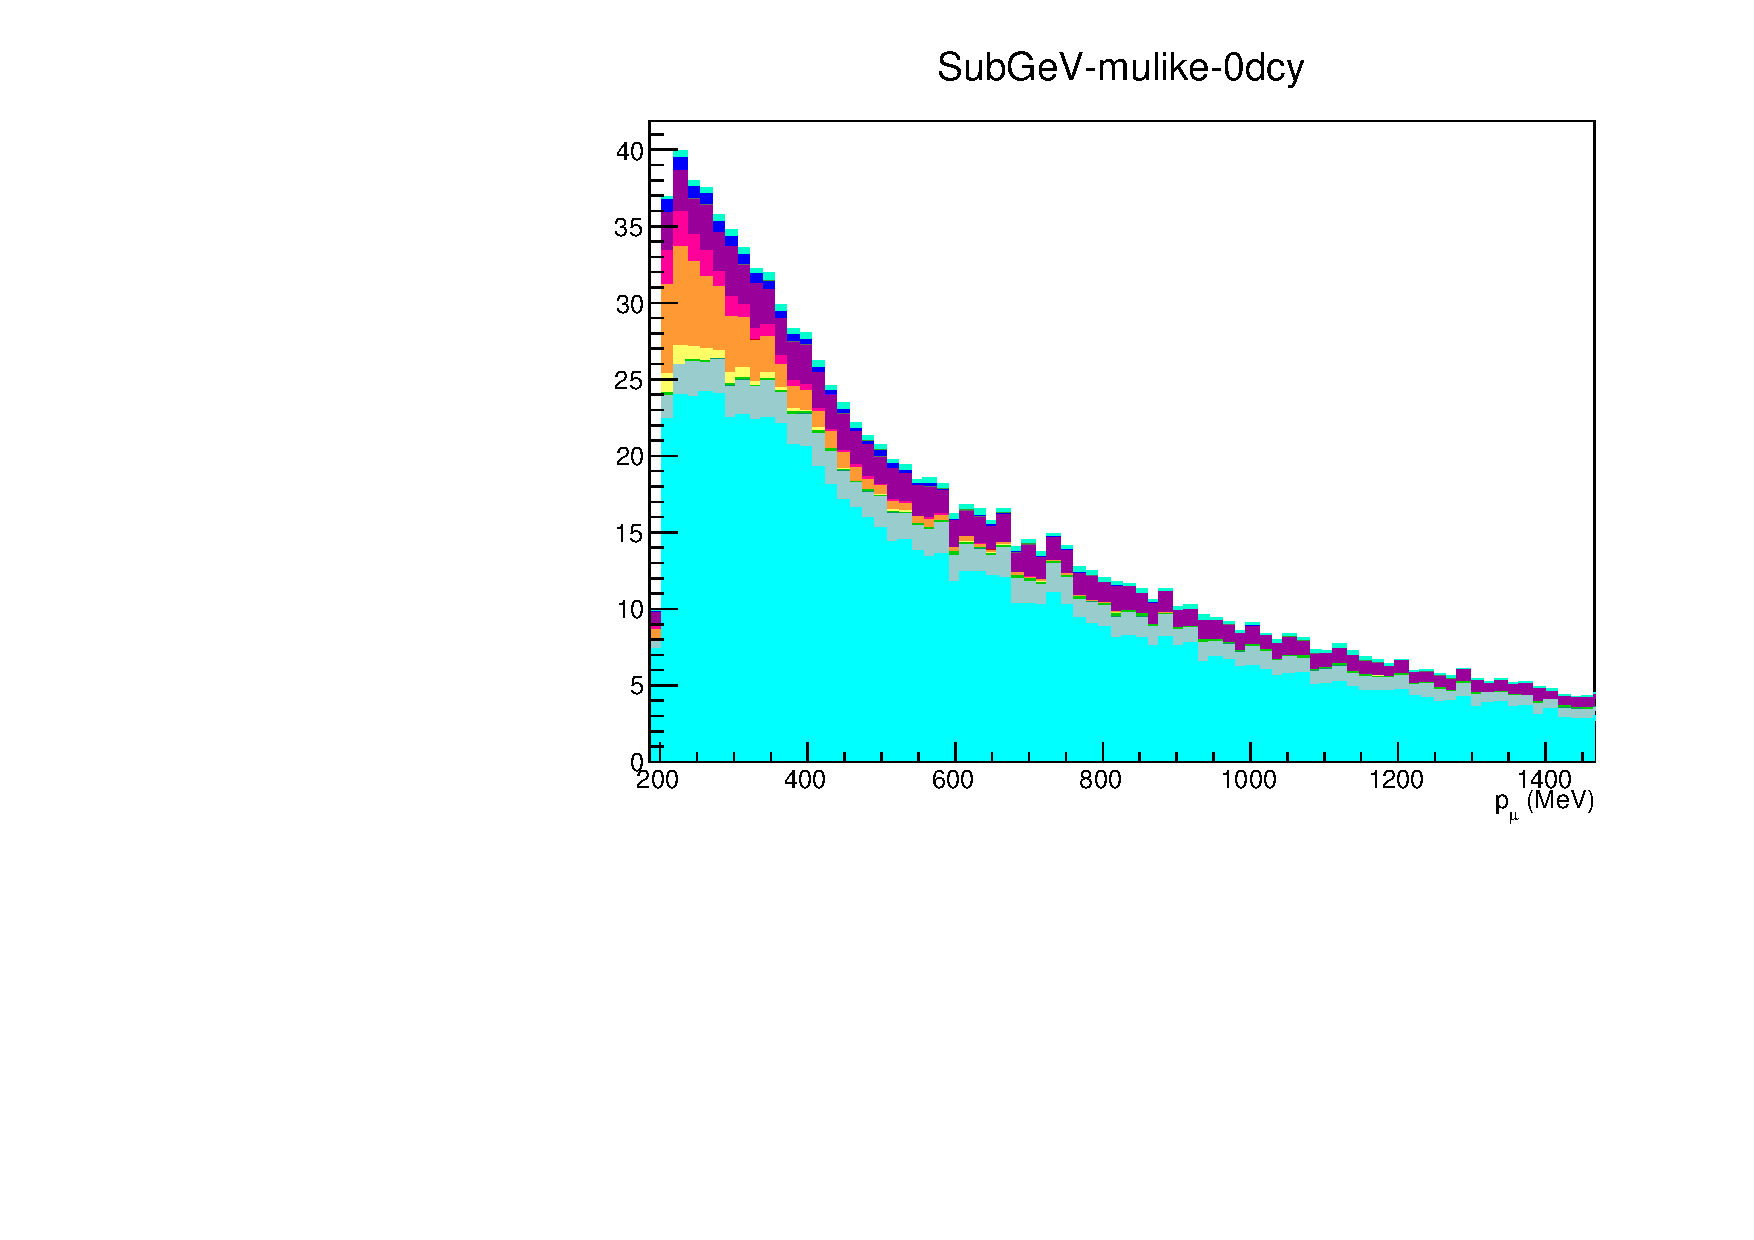
\includegraphics[width=\textwidth, trim= 0 0 0 30, clip]{Figures/Selections/AtmosphericByMode/SubGeV-mulike-0dcy_LepMom.pdf}
    \caption{FC Sub-GeV 1R $\mu$-like 0 de}
    \end{subfigure}
    \begin{subfigure}[t]{0.49\textwidth}
    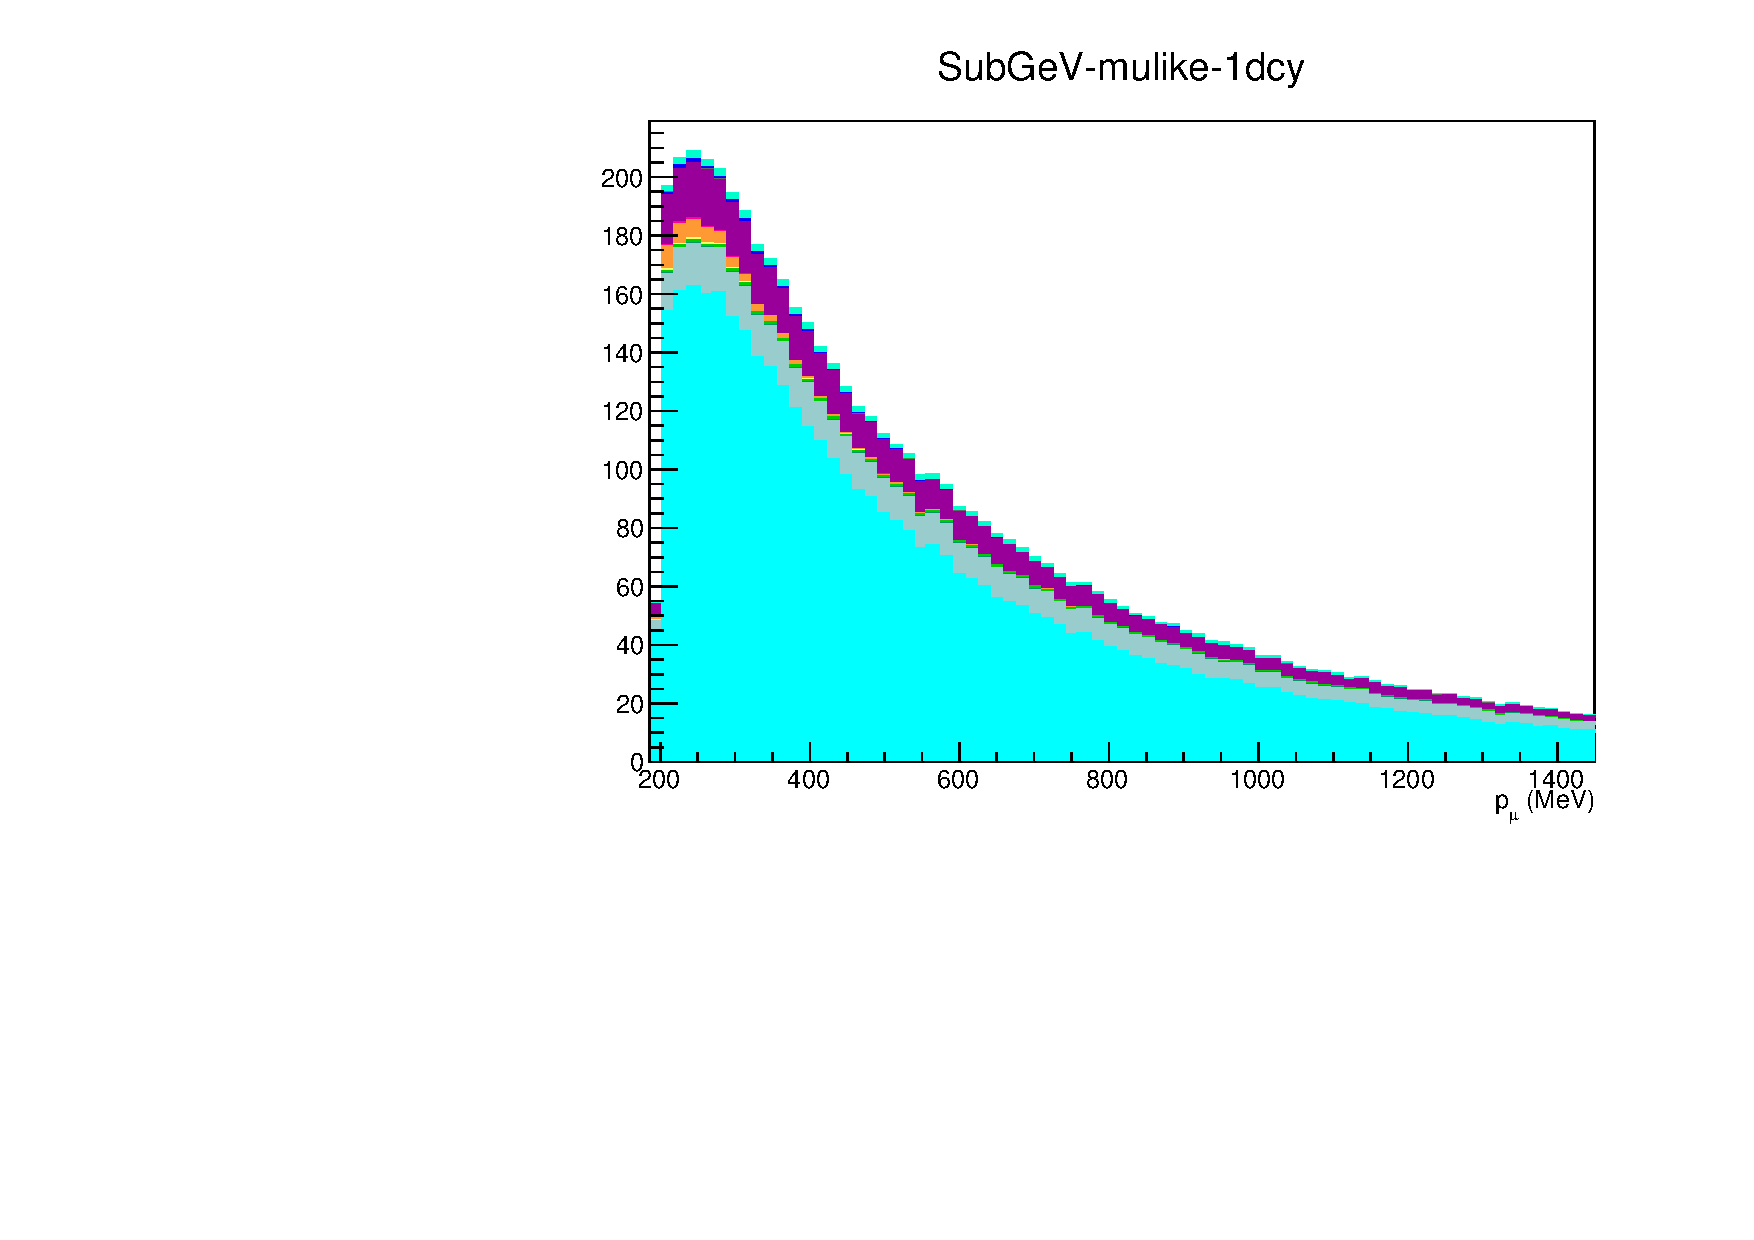
\includegraphics[width=\textwidth, trim= 0 0 0 30, clip]{Figures/Selections/AtmosphericByMode/SubGeV-mulike-1dcy_LepMom.pdf}
    \caption{FC Sub-GeV 1R $\mu$-like 1 de}
    \end{subfigure}
    \begin{subfigure}[t]{0.49\textwidth}
    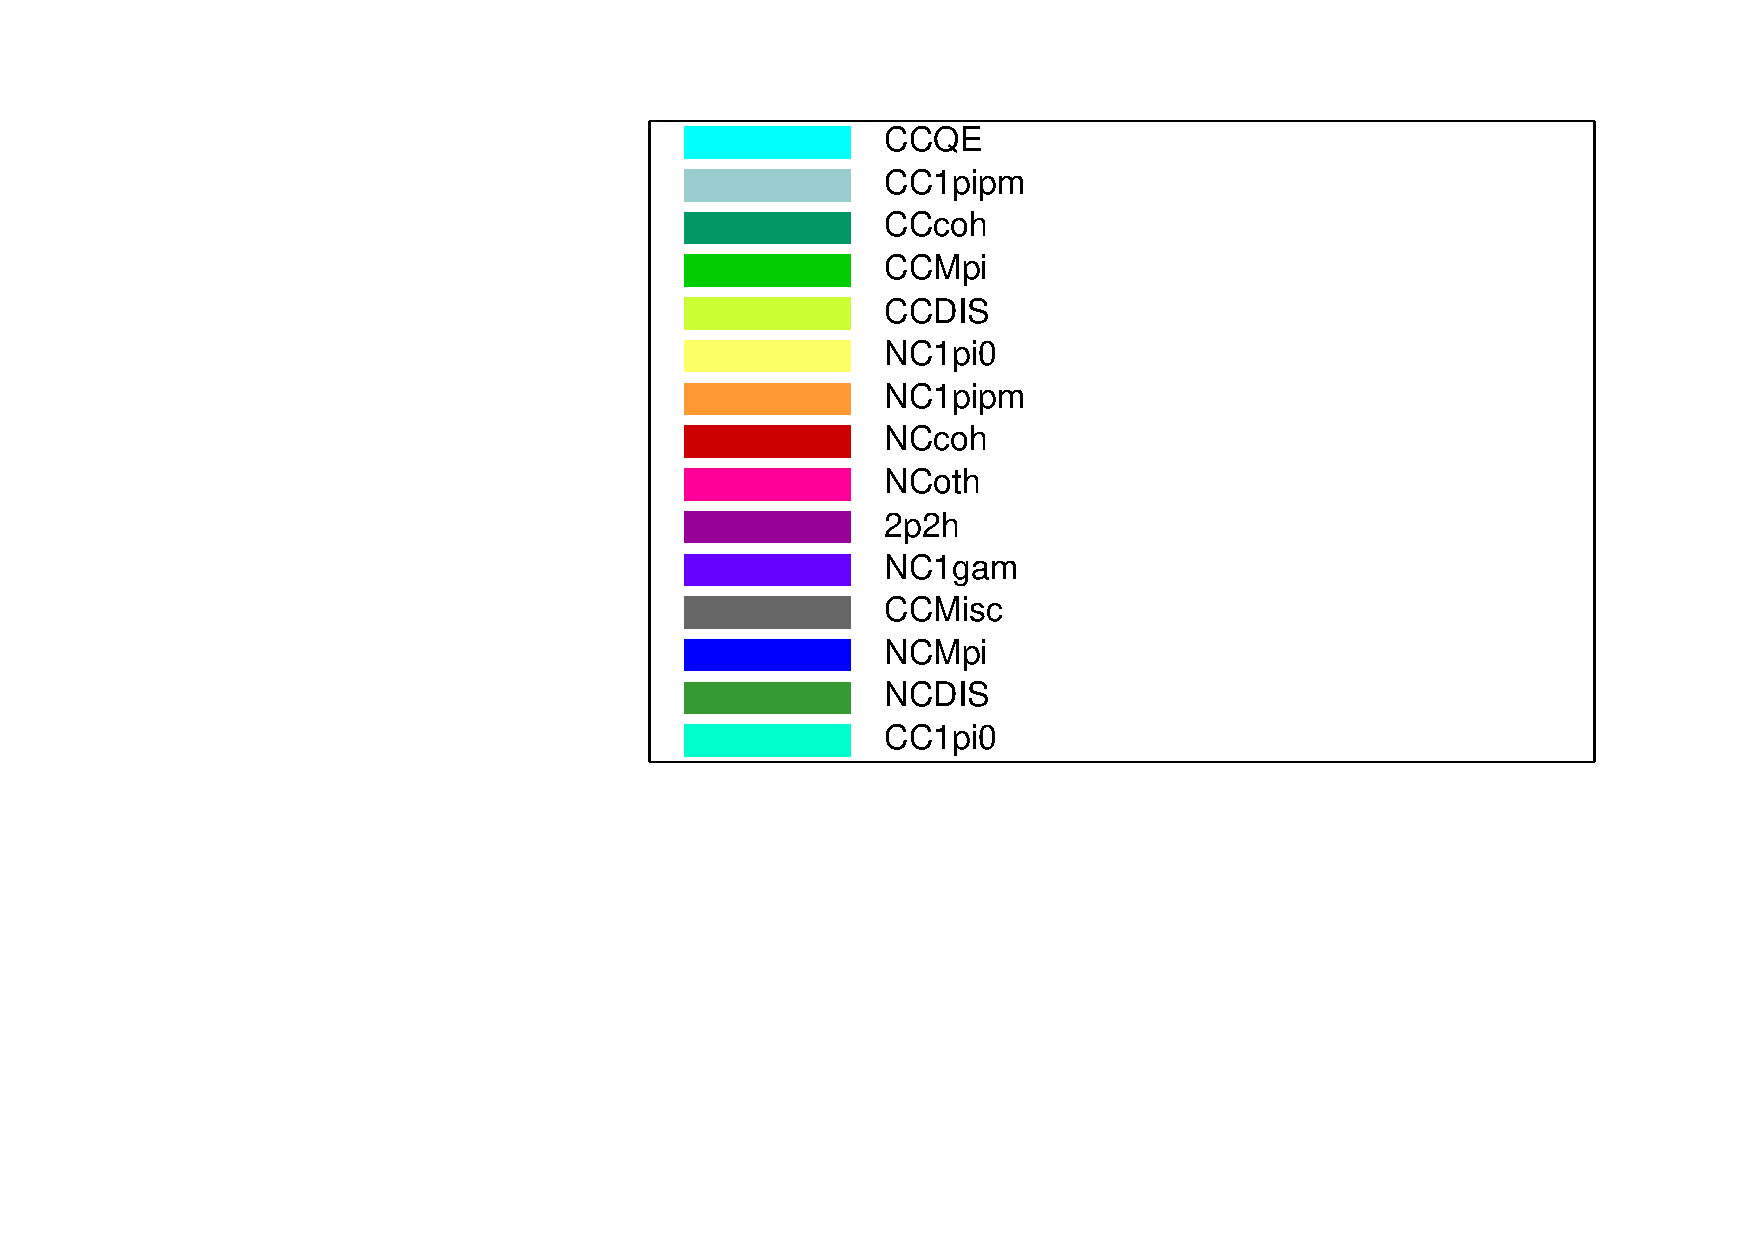
\includegraphics[page=1,width=\textwidth, trim= 0 0 0 30, clip]{Figures/Selections/AtmosphericByMode/Legend.pdf}
    \end{subfigure}
    \caption{Breakdown by interaction mode of the FC Sub-GeV atmospheric samples targeting CC0$\pi$ events.}
    \label{fig:SKSamples:FCSubGeVCC0pi}
\end{figure}

\begin{figure}[ht]
    \begin{subfigure}[t]{0.49\textwidth}
    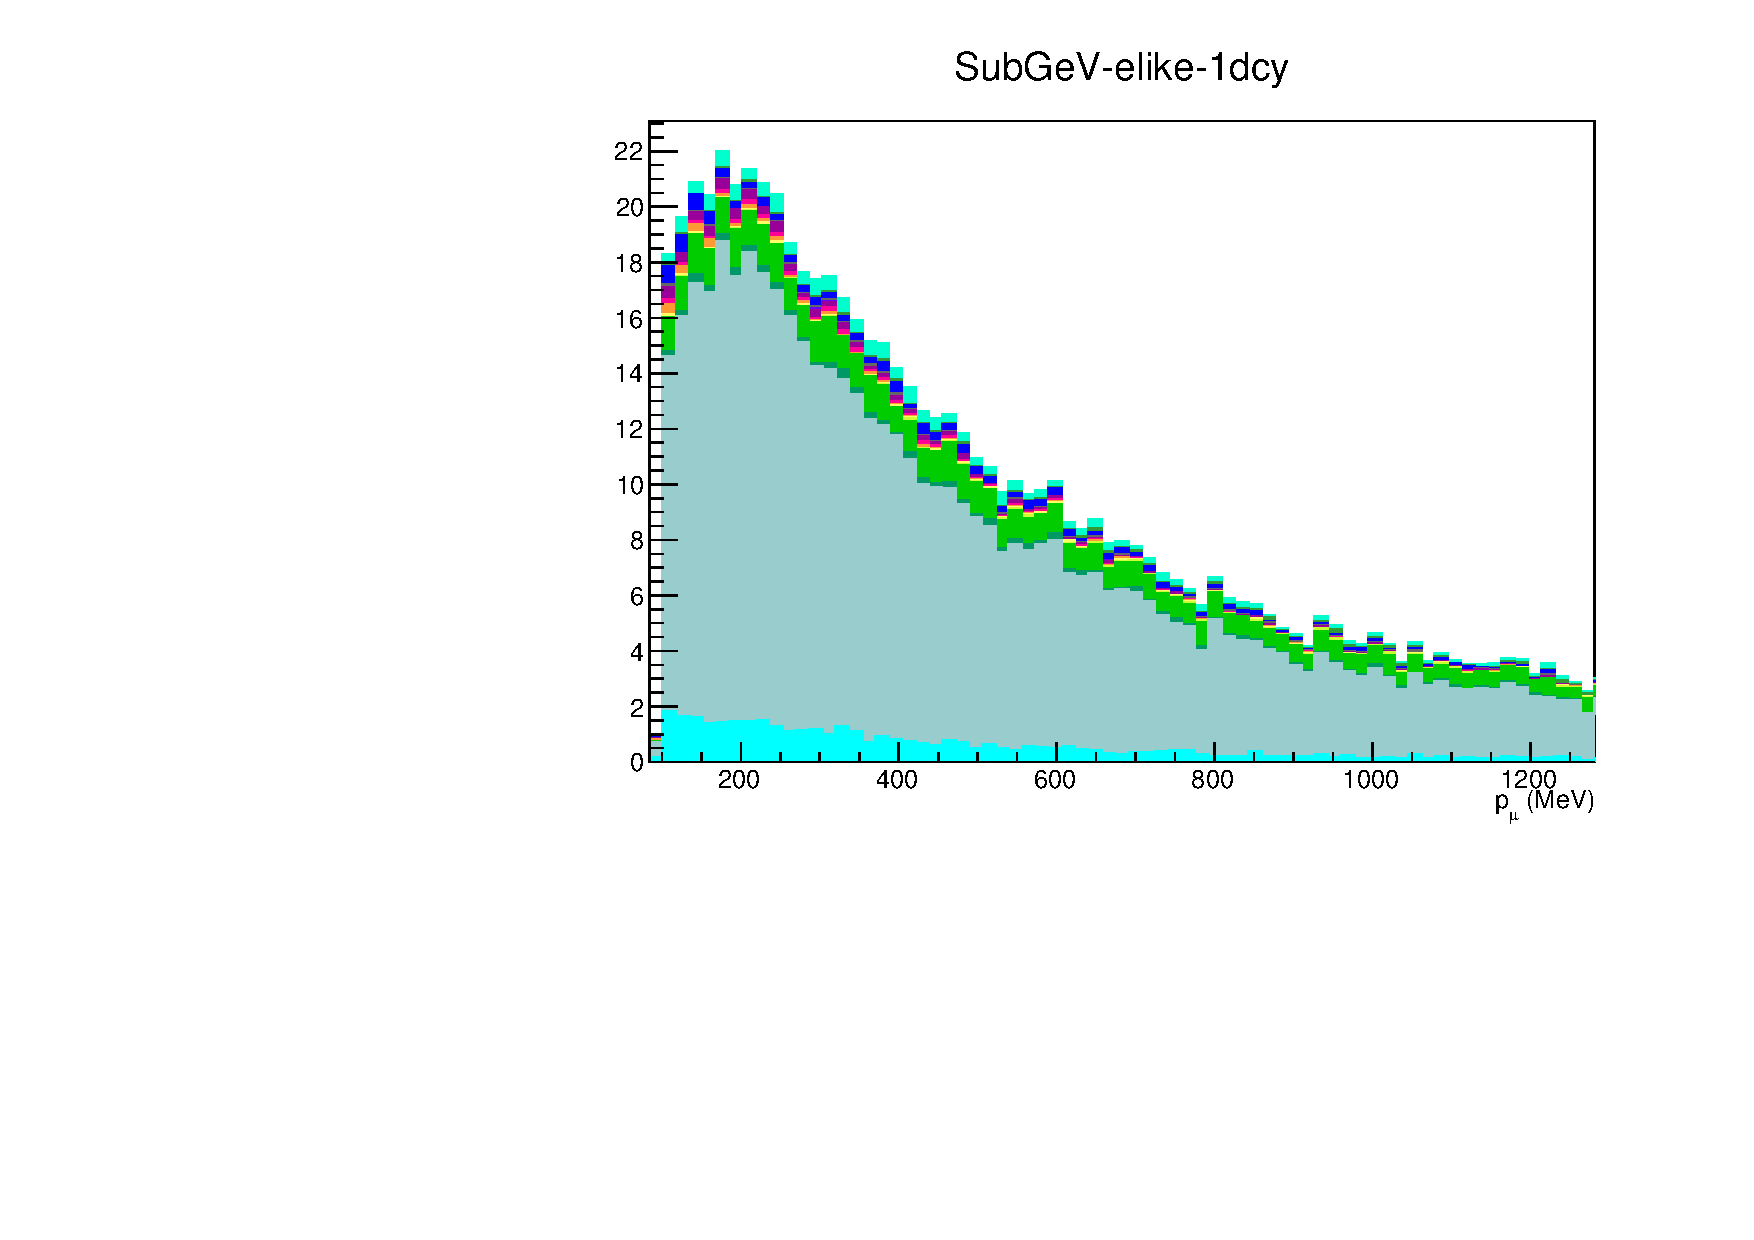
\includegraphics[width=\textwidth, trim= 0 0 0 30, clip]{Figures/Selections/AtmosphericByMode/SubGeV-elike-1dcy_LepMom.pdf}
    \caption{FC Sub-GeV 1R e-like 1 de}
    \end{subfigure}
    \begin{subfigure}[t]{0.49\textwidth}
    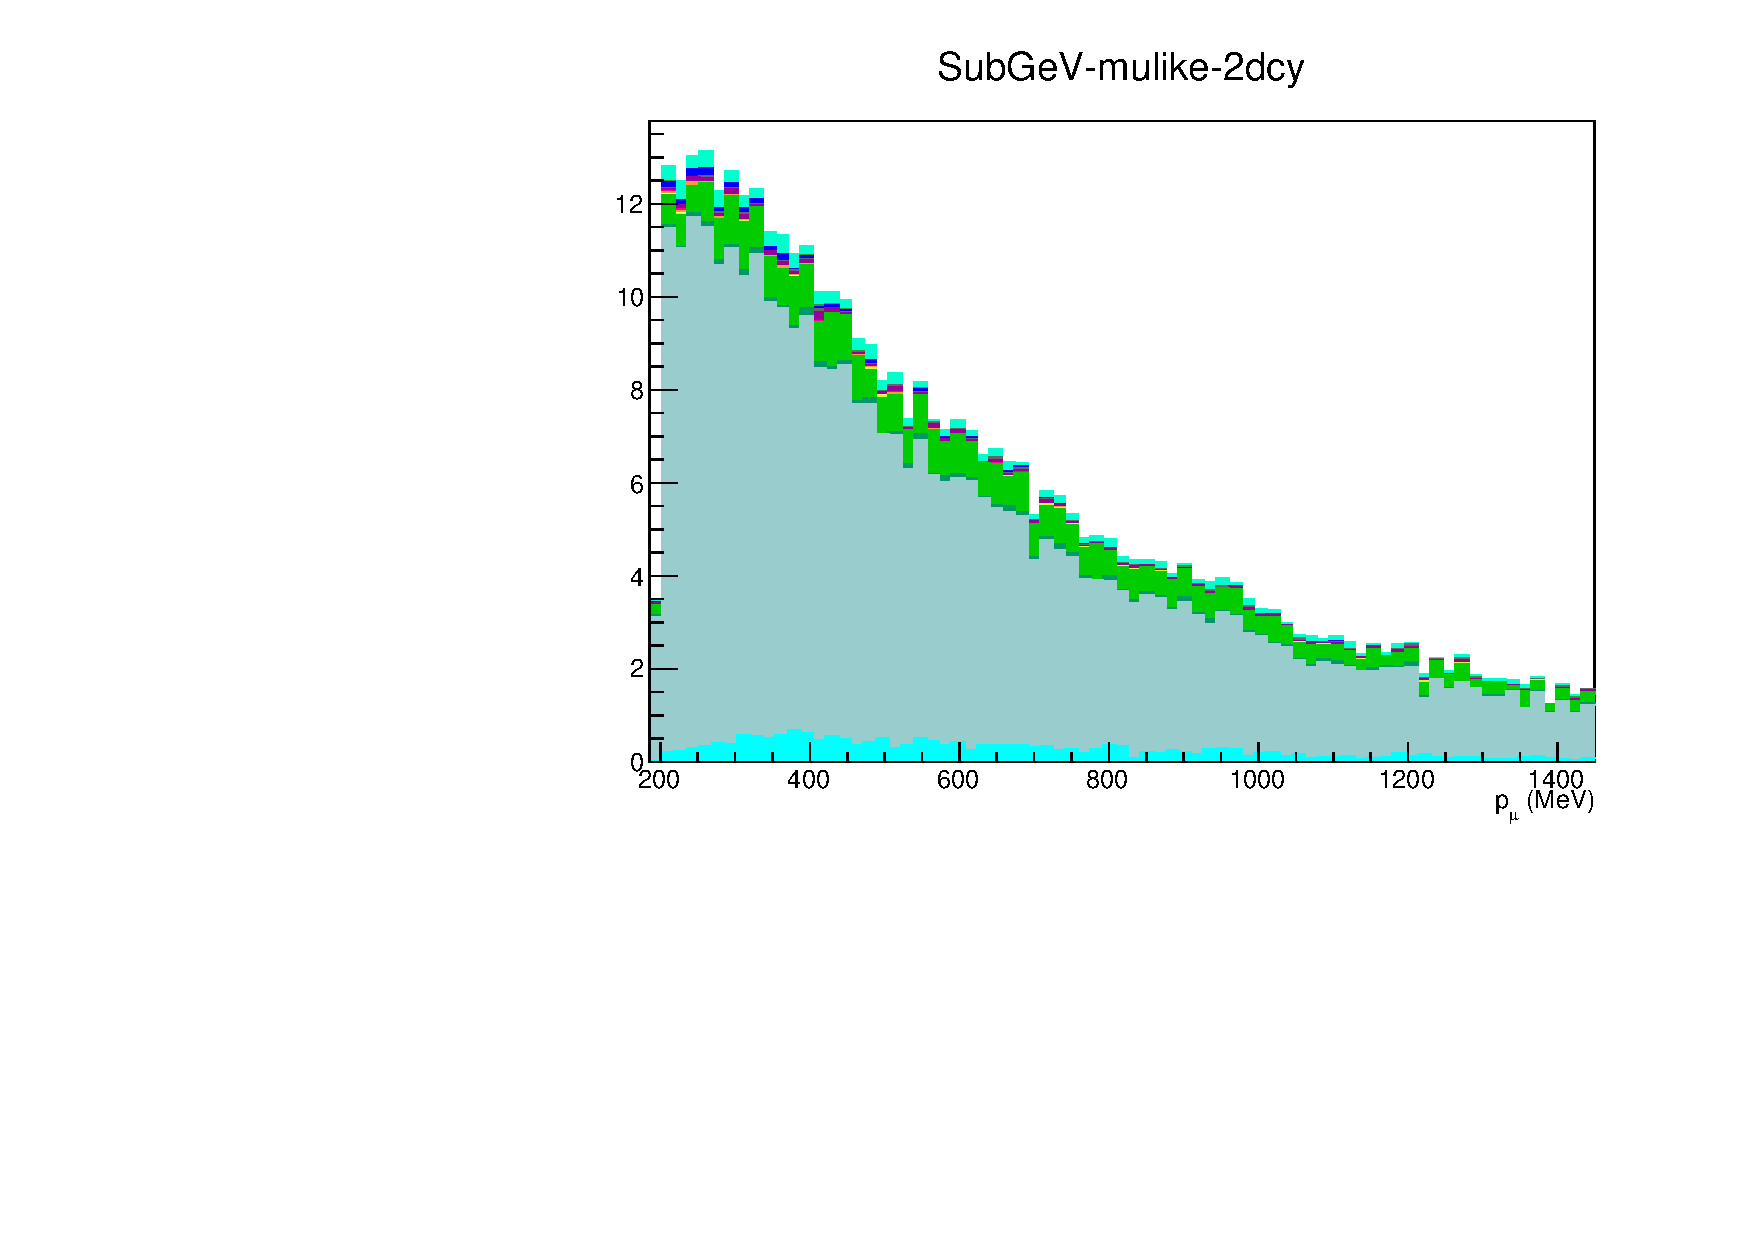
\includegraphics[width=\textwidth, trim= 0 0 0 30, clip]{Figures/Selections/AtmosphericByMode/SubGeV-mulike-2dcy_LepMom.pdf}
    \caption{FC Sub-GeV 1R $\mu$-like 2 de}
    \end{subfigure}
    \begin{subfigure}[t]{0.49\textwidth}
    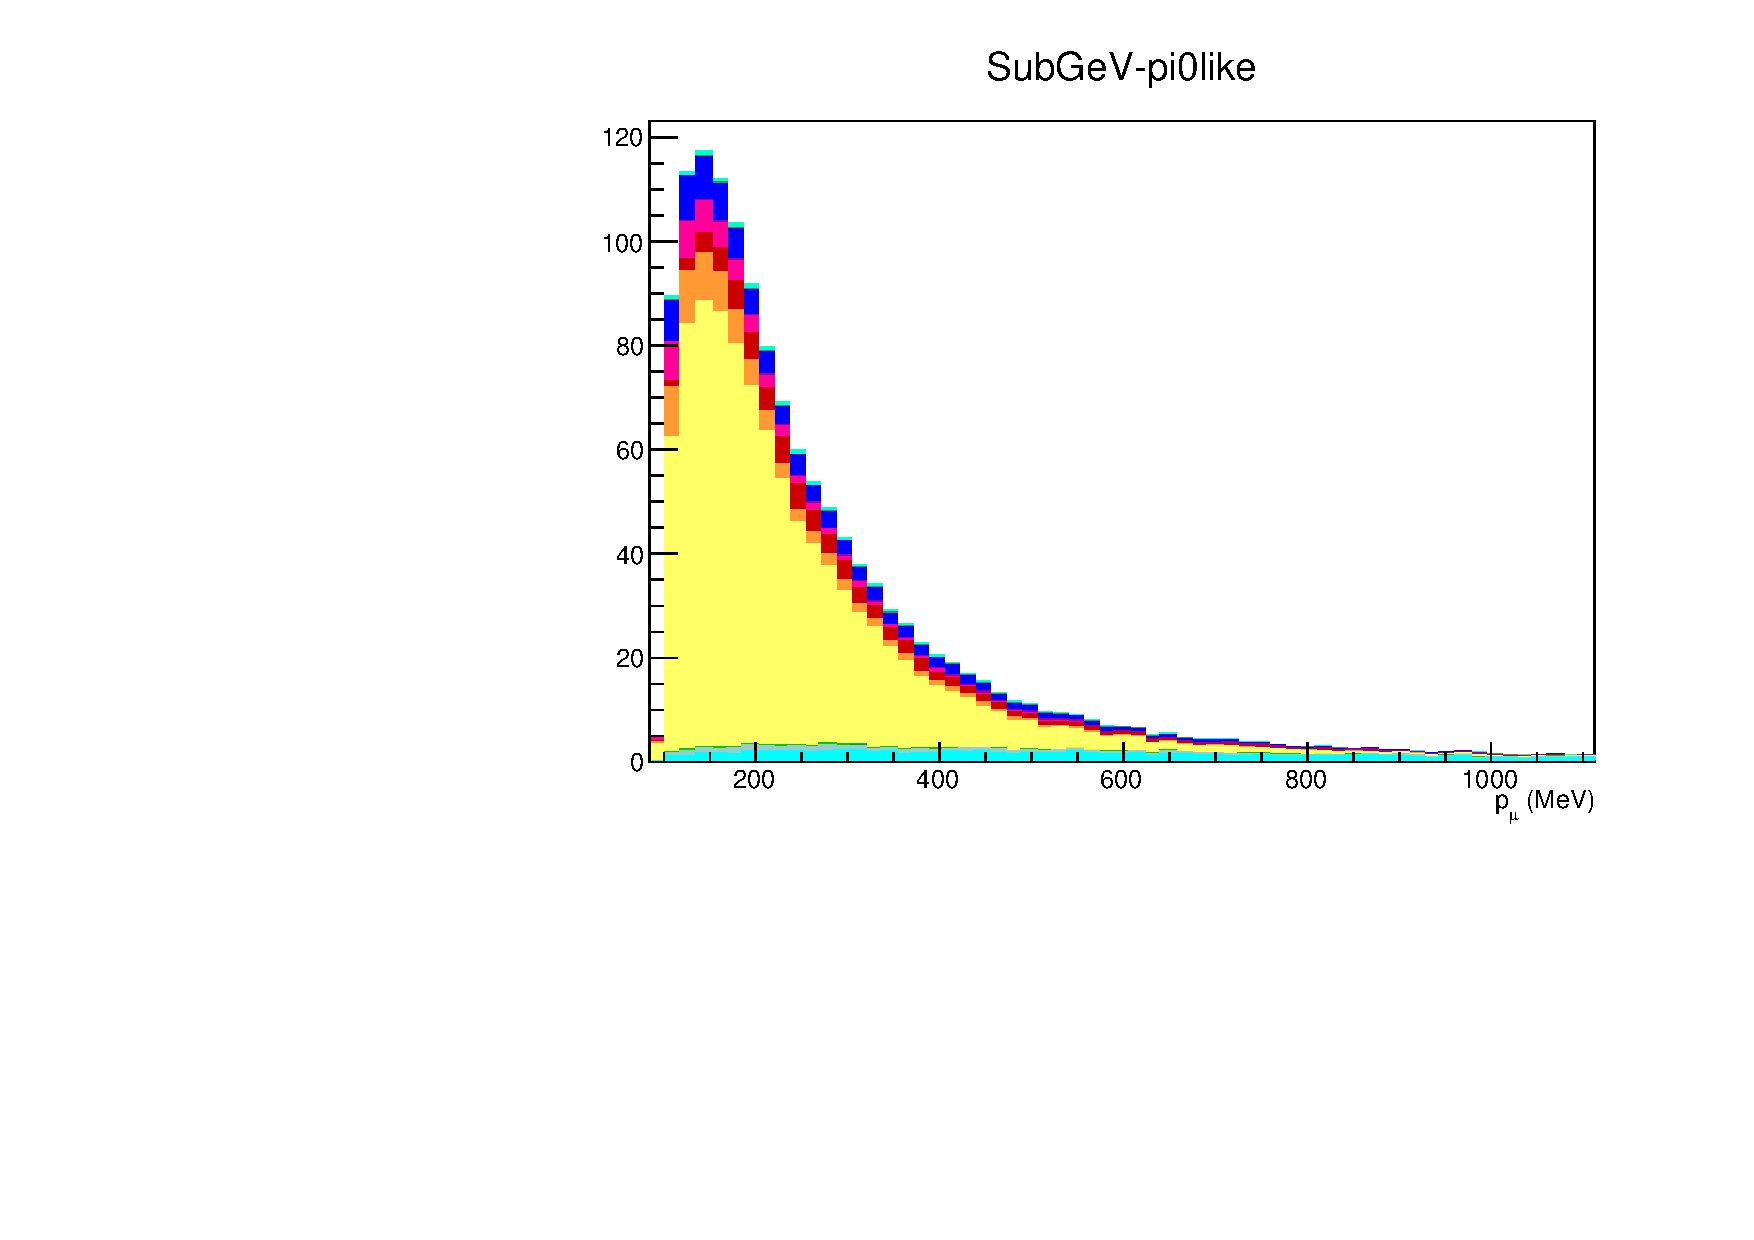
\includegraphics[width=\textwidth, trim= 0 0 0 30, clip]{Figures/Selections/AtmosphericByMode/SubGeV-pi0like_LepMom.pdf}
    \caption{FC Sub-GeV 2R $\pi^{0}$-like}
    \end{subfigure}
    \begin{subfigure}[t]{0.49\textwidth}
    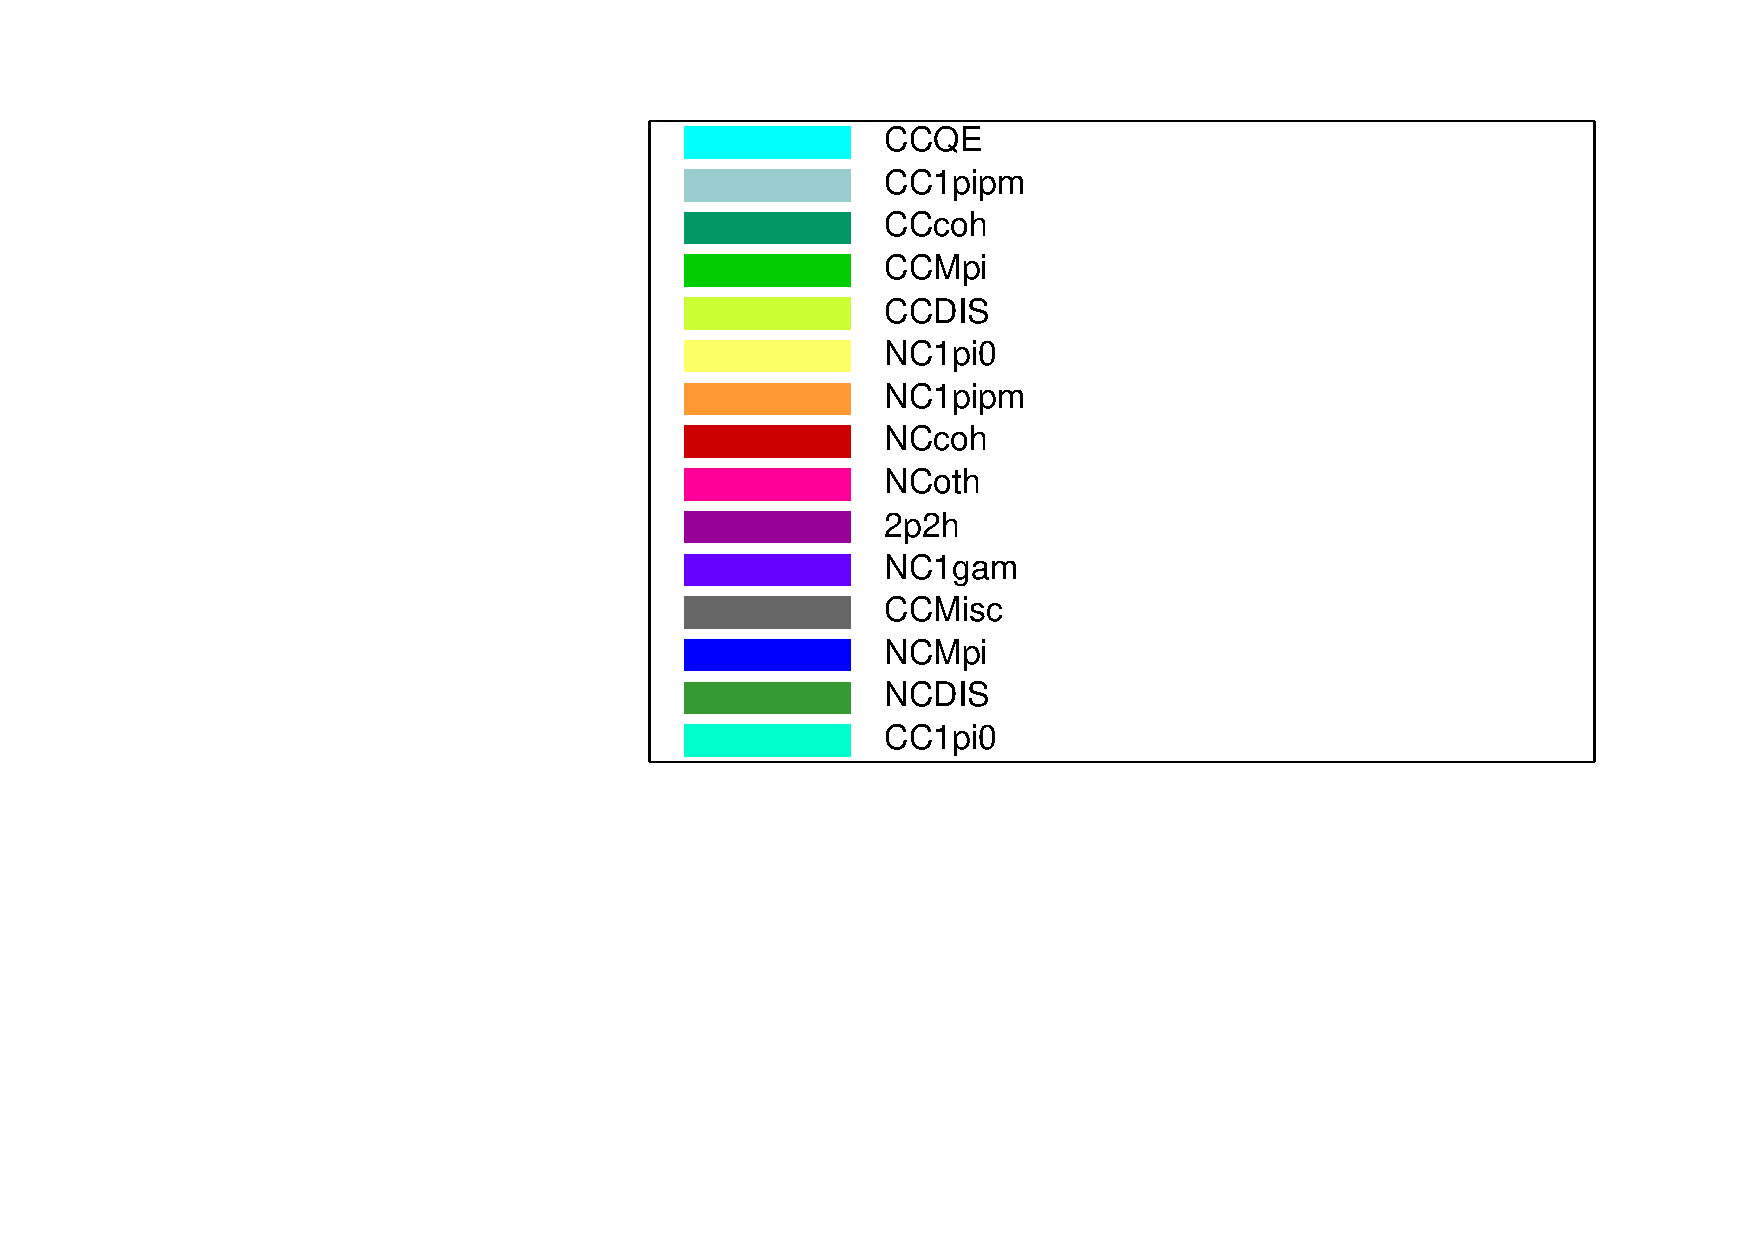
\includegraphics[page=1,width=\textwidth, trim= 0 0 0 30, clip]{Figures/Selections/AtmosphericByMode/Legend.pdf}
    \end{subfigure}
    \caption{Breakdown by interaction mode of the FC Sub-GeV atmospheric samples targeting single pion events.}
    \label{fig:SKSamples:FCSubGeVCC1pi}
\end{figure}

\clearpage
\section{Fully Contained Multi-GeV Samples}
The interaction mode breakdown of fully contained multi-GeV samples is highlighted in \autoref{fig:SKSamples:FCMultiGeV}. Due to the event selection applied in SK which targets $\pi^+$ and $\pi^-$ separation, the $\nu_e$ sample mainly consists of events with pions (single pion production or multi-pion/DIS interactions). The pion separation is explained in Section \autoref{sec:SelsAndSysts_Sels_Atms}. This reasoning also explains the significant CCQE contribution of the $\bar{\nu}_e$ sample. The muon-like sample is dominated by CCQE interactions with $\sim10-15\%$ 2p2h and CC1$\pi$ contribution of events.

\begin{figure}[ht]
    \begin{subfigure}[t]{0.49\textwidth}
    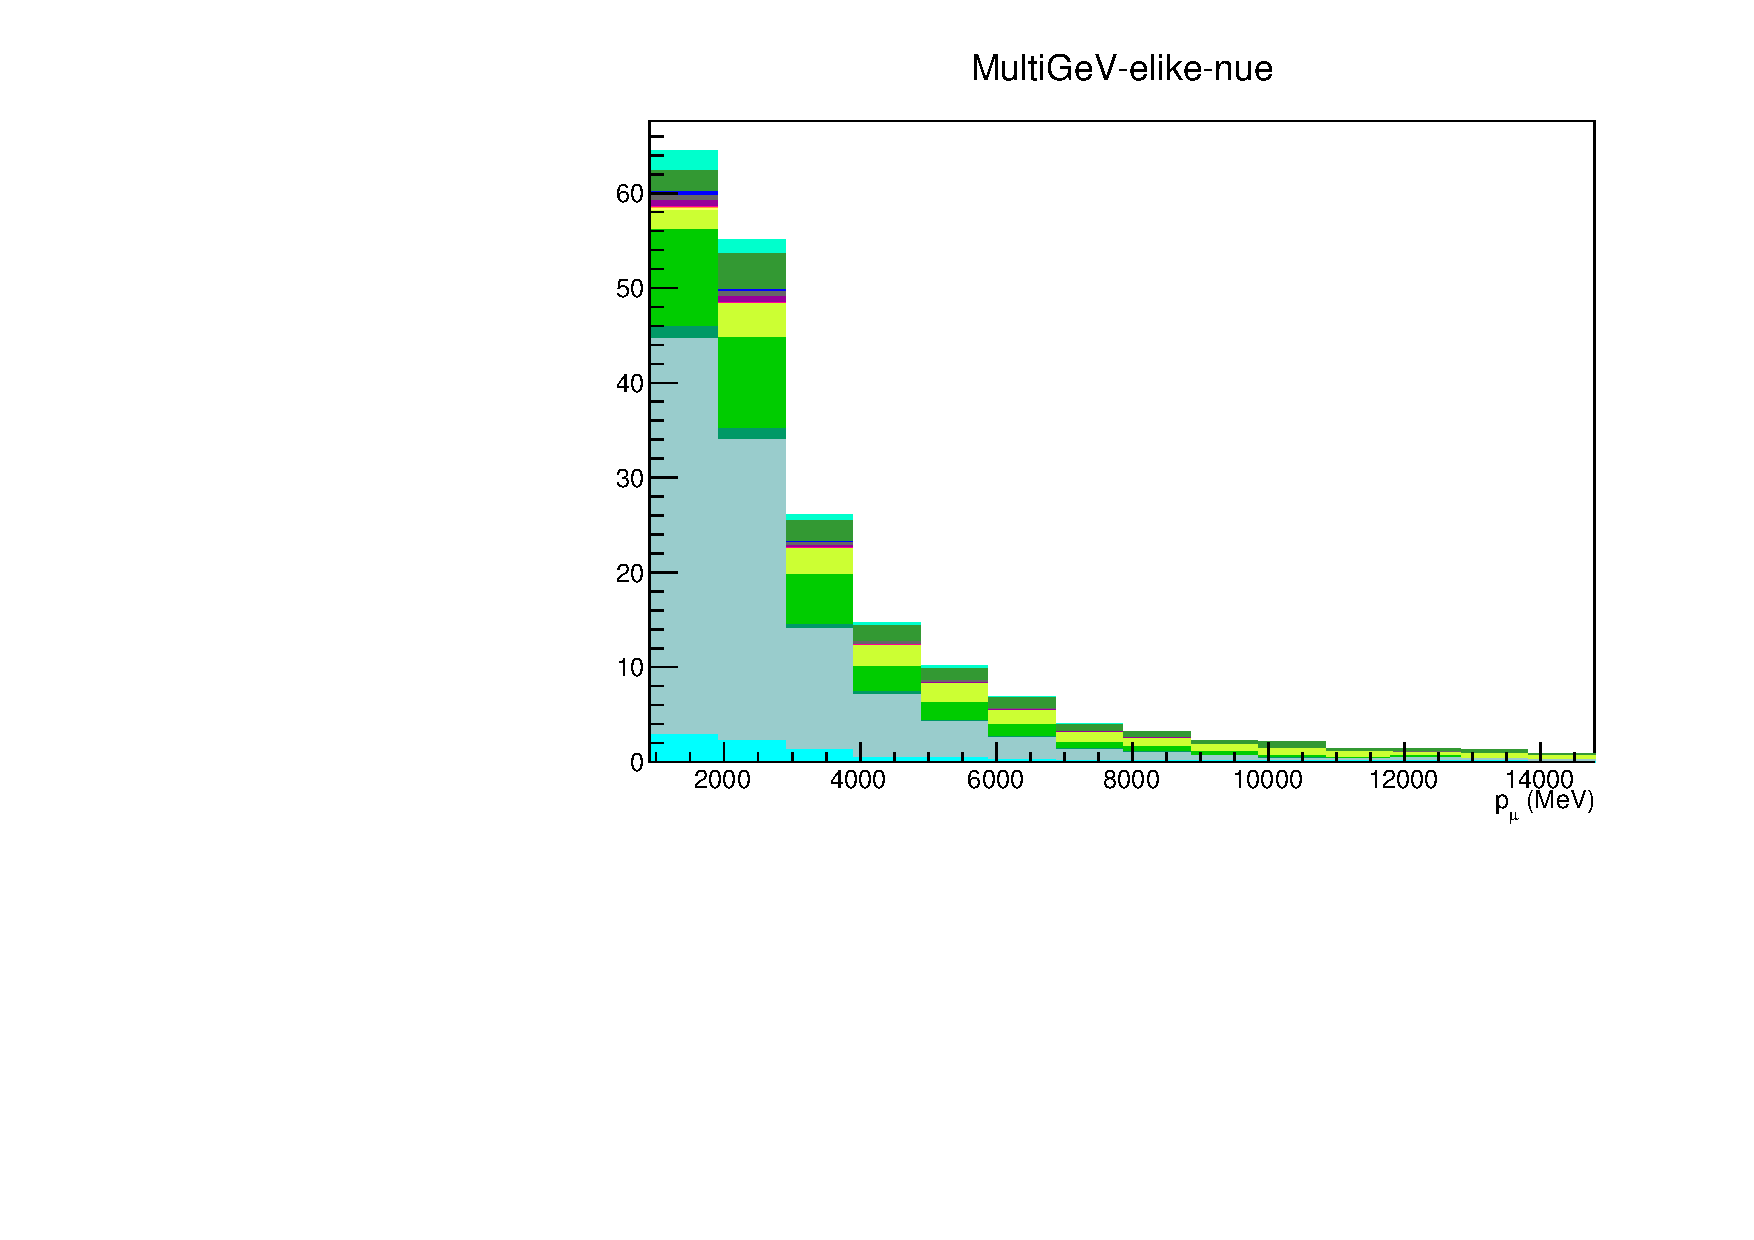
\includegraphics[width=\textwidth, trim= 0 0 0 30, clip]{Figures/Selections/AtmosphericByMode/MultiGeV-elike-nue_LepMom.pdf}
    \caption{FC Multi-GeV single ring $\nu_e$-like}
    \end{subfigure}
    \begin{subfigure}[t]{0.49\textwidth}
    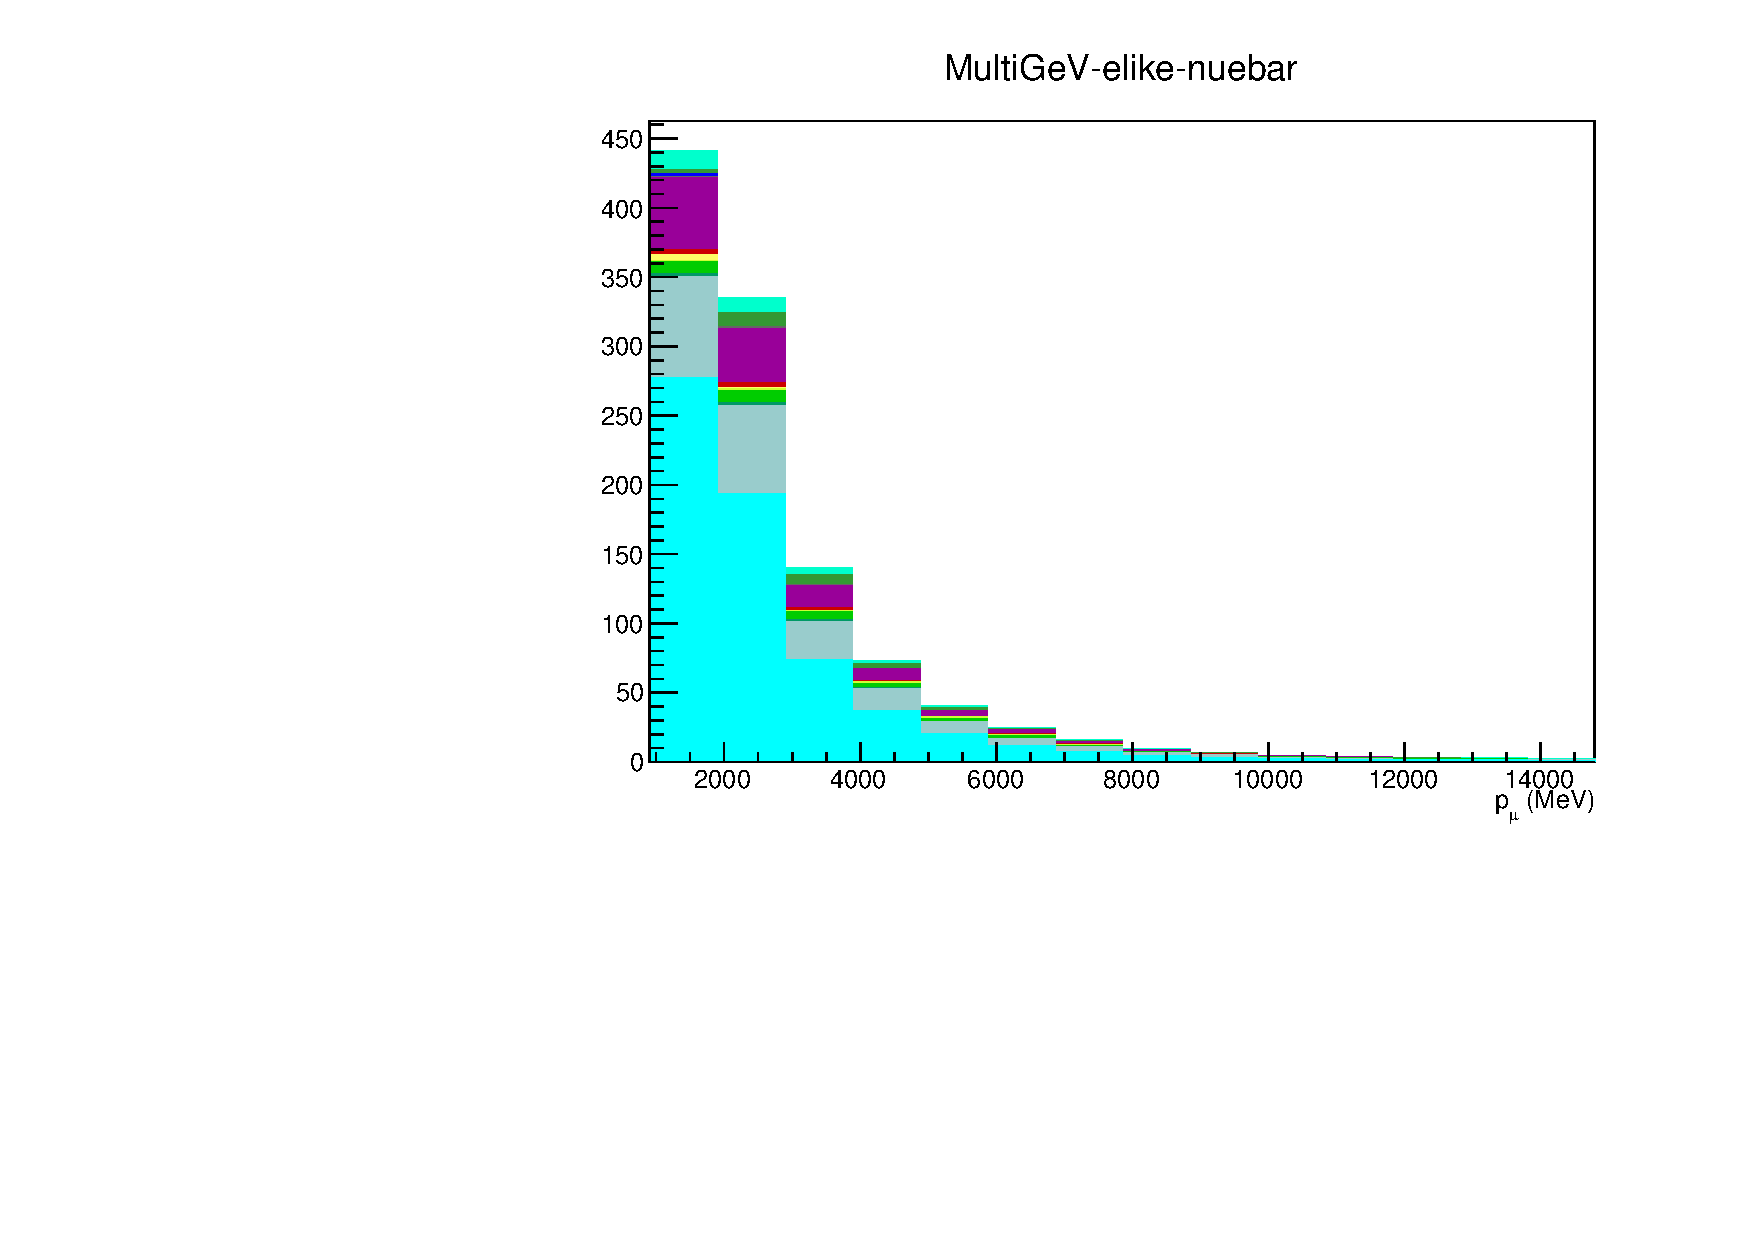
\includegraphics[width=\textwidth, trim= 0 0 0 30, clip]{Figures/Selections/AtmosphericByMode/MultiGeV-elike-nuebar_LepMom.pdf}
    \caption{FC Multi-GeV single ring $\bar{\nu}_e$-like}
    \end{subfigure}
    \begin{subfigure}[t]{0.49\textwidth}
    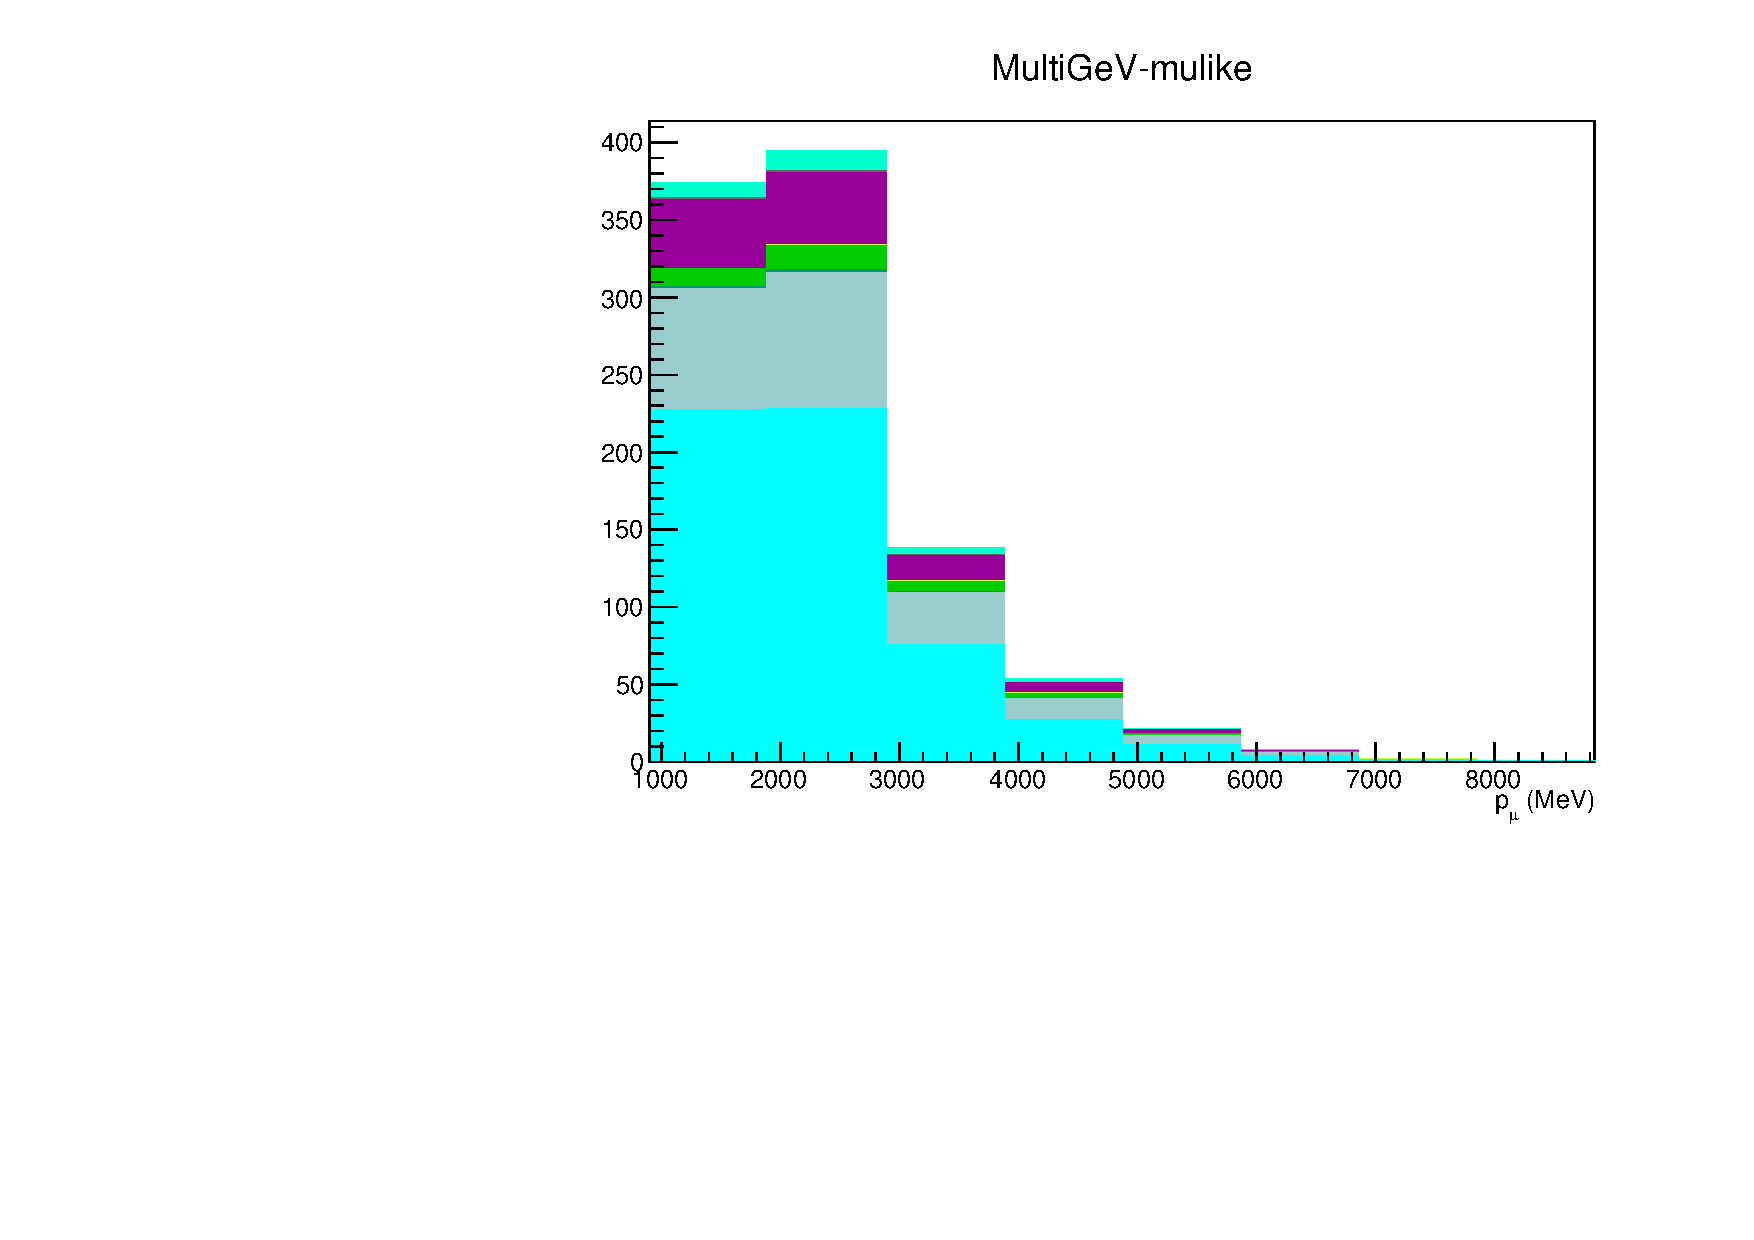
\includegraphics[width=\textwidth, trim= 0 0 0 30, clip]{Figures/Selections/AtmosphericByMode/MultiGeV-mulike_LepMom.pdf}
    \caption{FC Multi-GeV single ring $\mu$-like}
    \end{subfigure}
    \begin{subfigure}[t]{0.49\textwidth}
    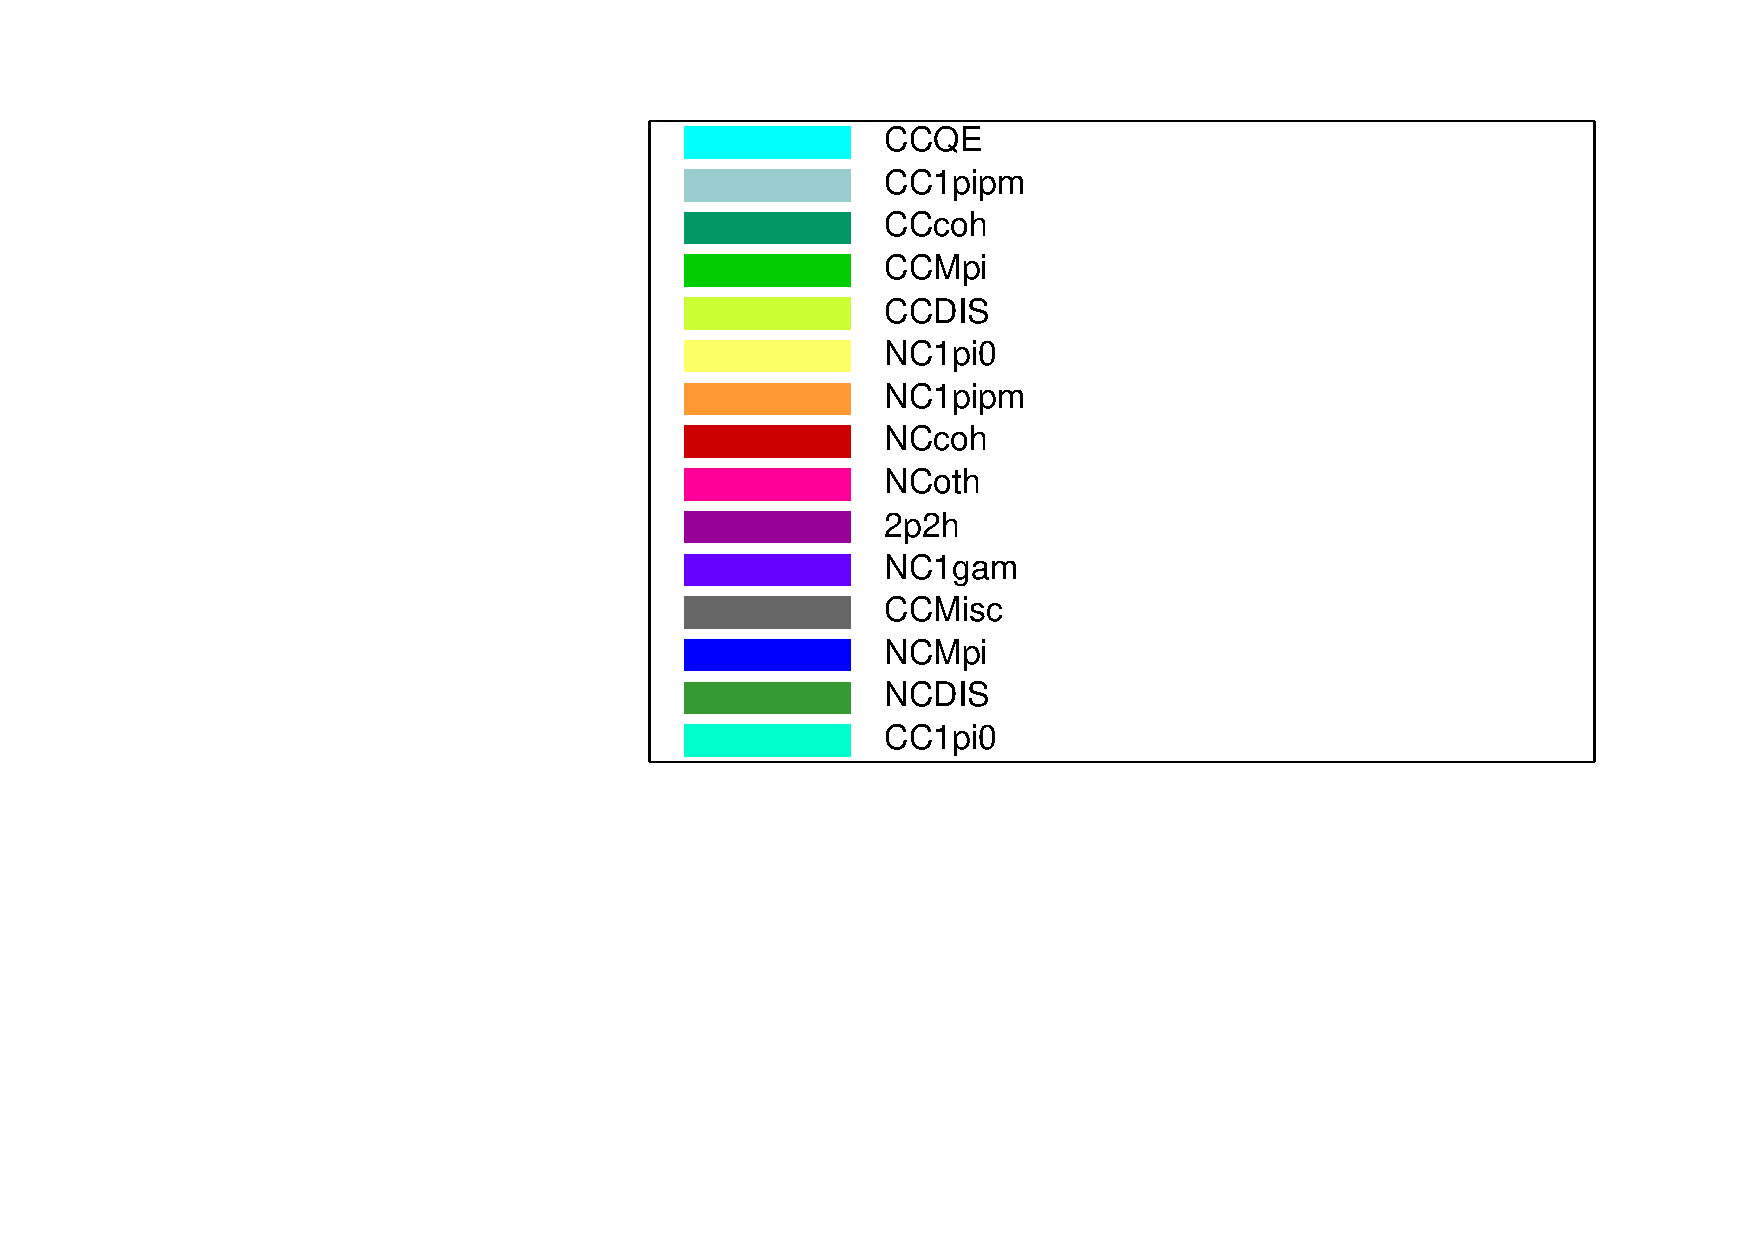
\includegraphics[page=1,width=\textwidth, trim= 0 0 0 30, clip]{Figures/Selections/AtmosphericByMode/Legend.pdf}
    \end{subfigure}

    \caption{Breakdown by interaction mode of the FC Multi-GeV single ring atmospheric samples.}
    \label{fig:SKSamples:FCMultiGeV}
\end{figure}

\clearpage
\section{Fully Contained Multi-Ring Samples}

The interaction mode breakdown of fully contained multi-ring events is shown in \autoref{fig:SKSamples:FCMultiRing}. These samples see more interaction modes contributing in general, and there is a much larger contribution from multi-pion and DIS interaction modes, compared to the other samples.

\begin{figure}[ht]
    \begin{subfigure}[t]{0.49\textwidth}
    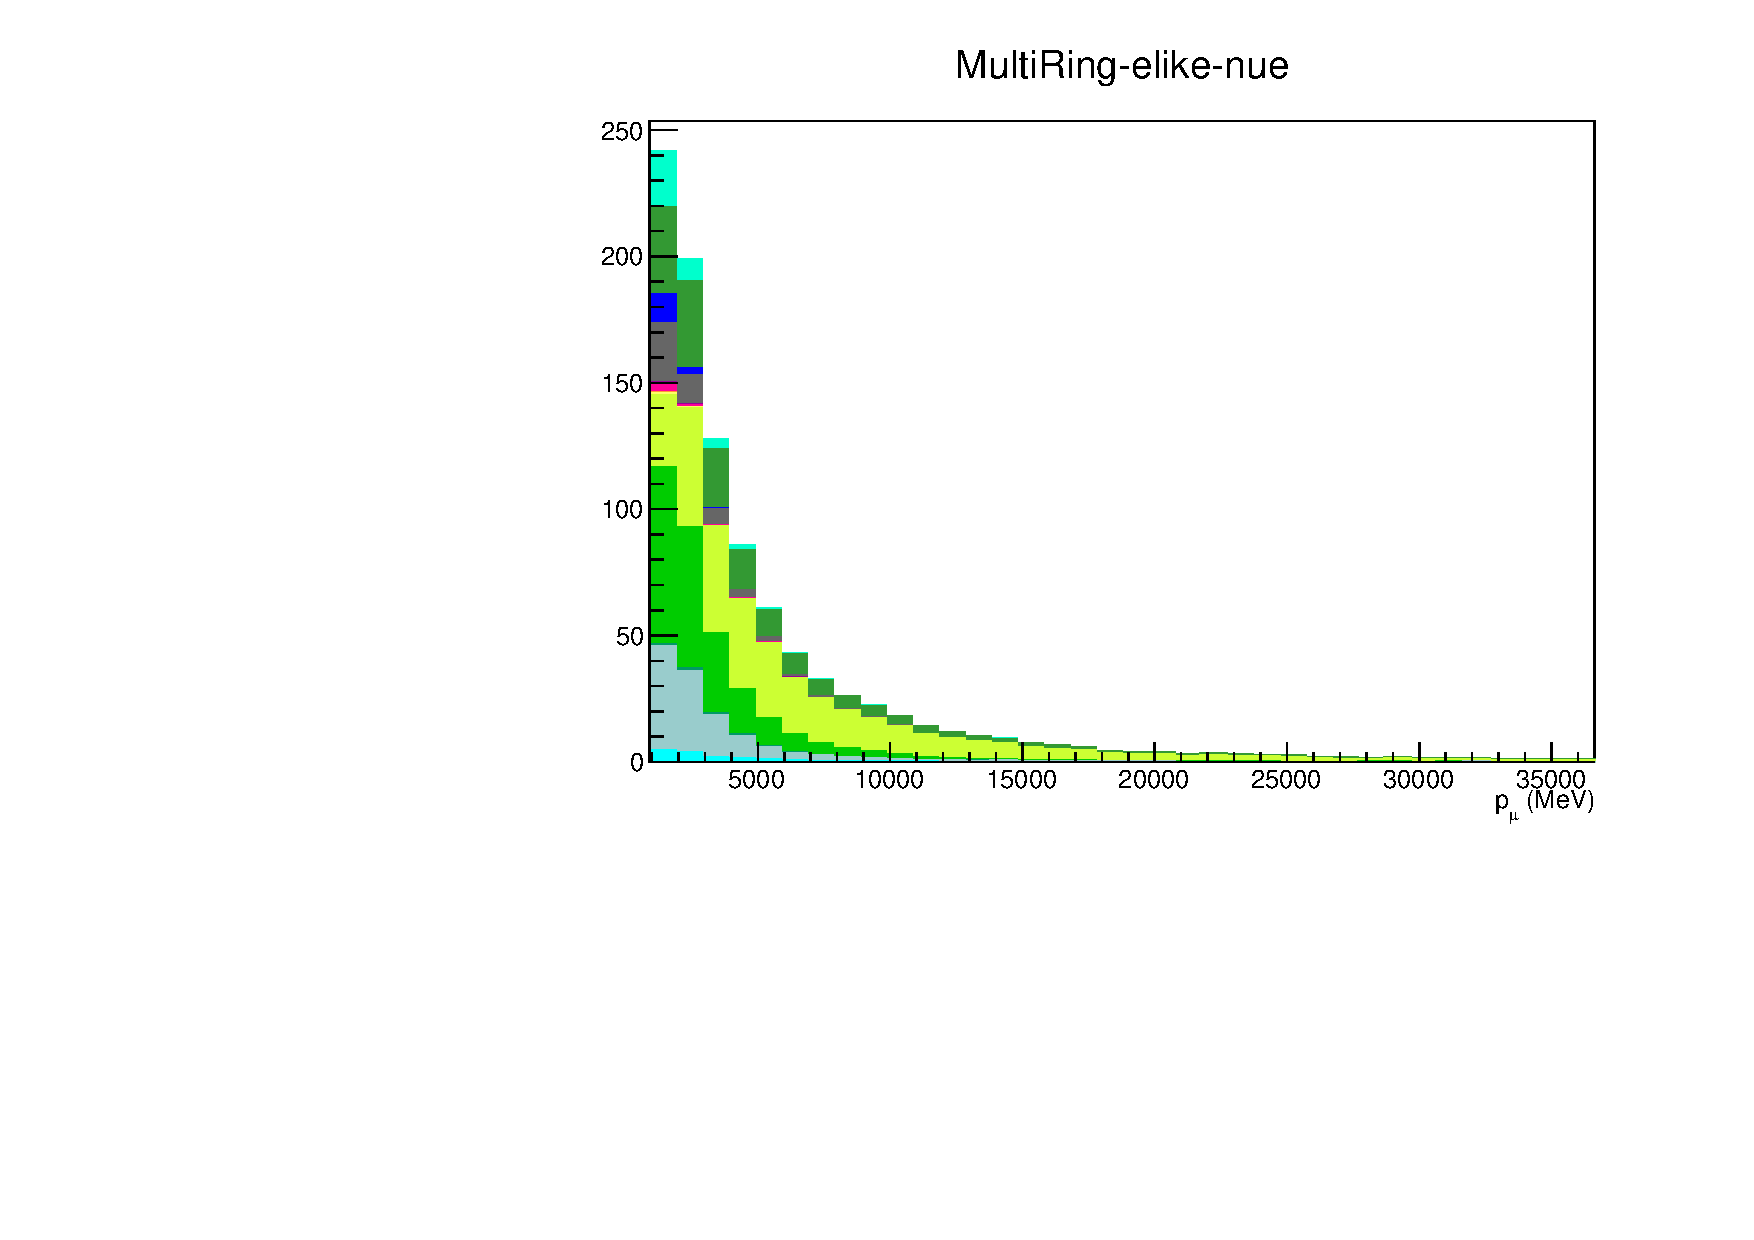
\includegraphics[width=\textwidth, trim= 0 0 0 30, clip]{Figures/Selections/AtmosphericByMode/MultiRing-elike-nue_LepMom.pdf}
    \caption{FC Multi-GeV multi-ring $\nu_e$-like}
    \end{subfigure}
    \begin{subfigure}[t]{0.49\textwidth}
    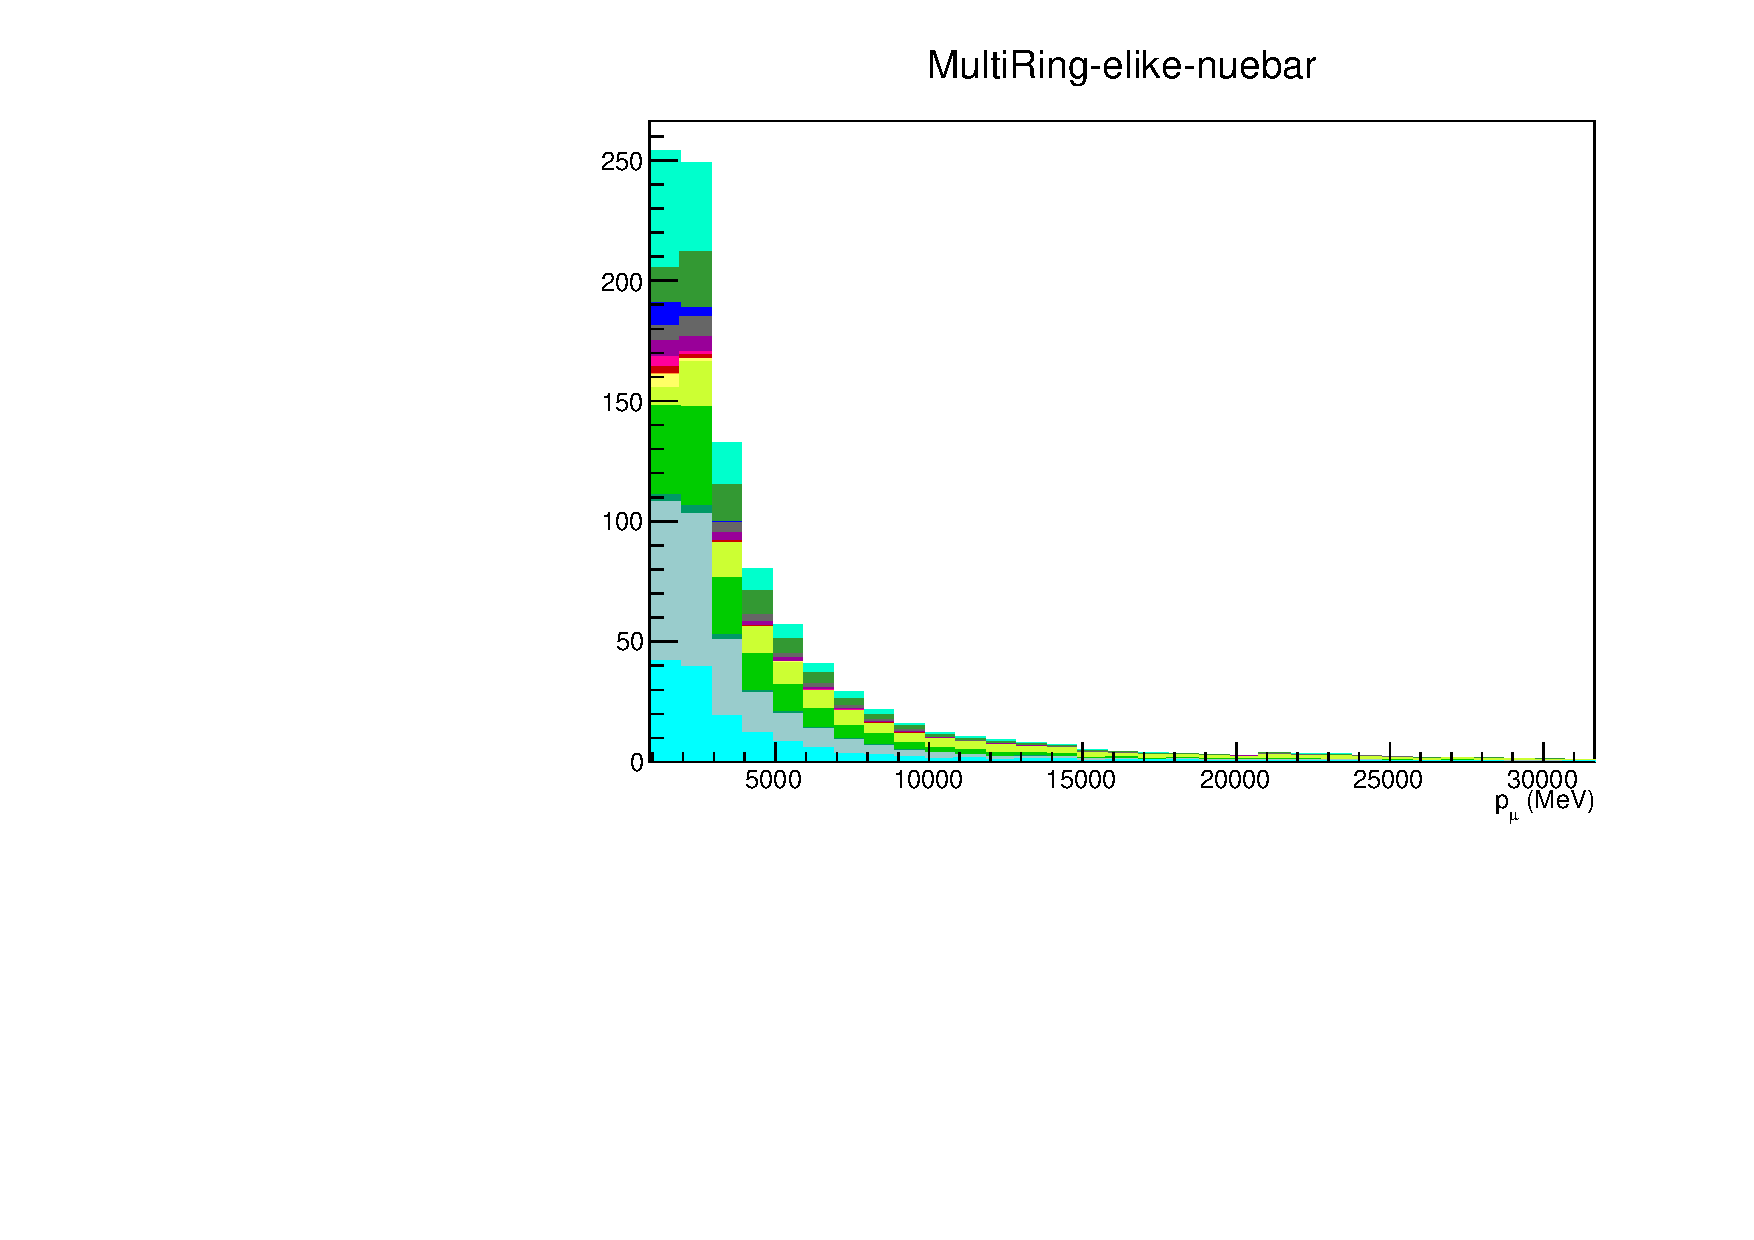
\includegraphics[width=\textwidth, trim= 0 0 0 30, clip]{Figures/Selections/AtmosphericByMode/MultiRing-elike-nuebar_LepMom.pdf}
    \caption{FC Multi-GeV multi-ring $\bar{\nu}_e$-like}
    \end{subfigure}
    \begin{subfigure}[t]{0.49\textwidth}
    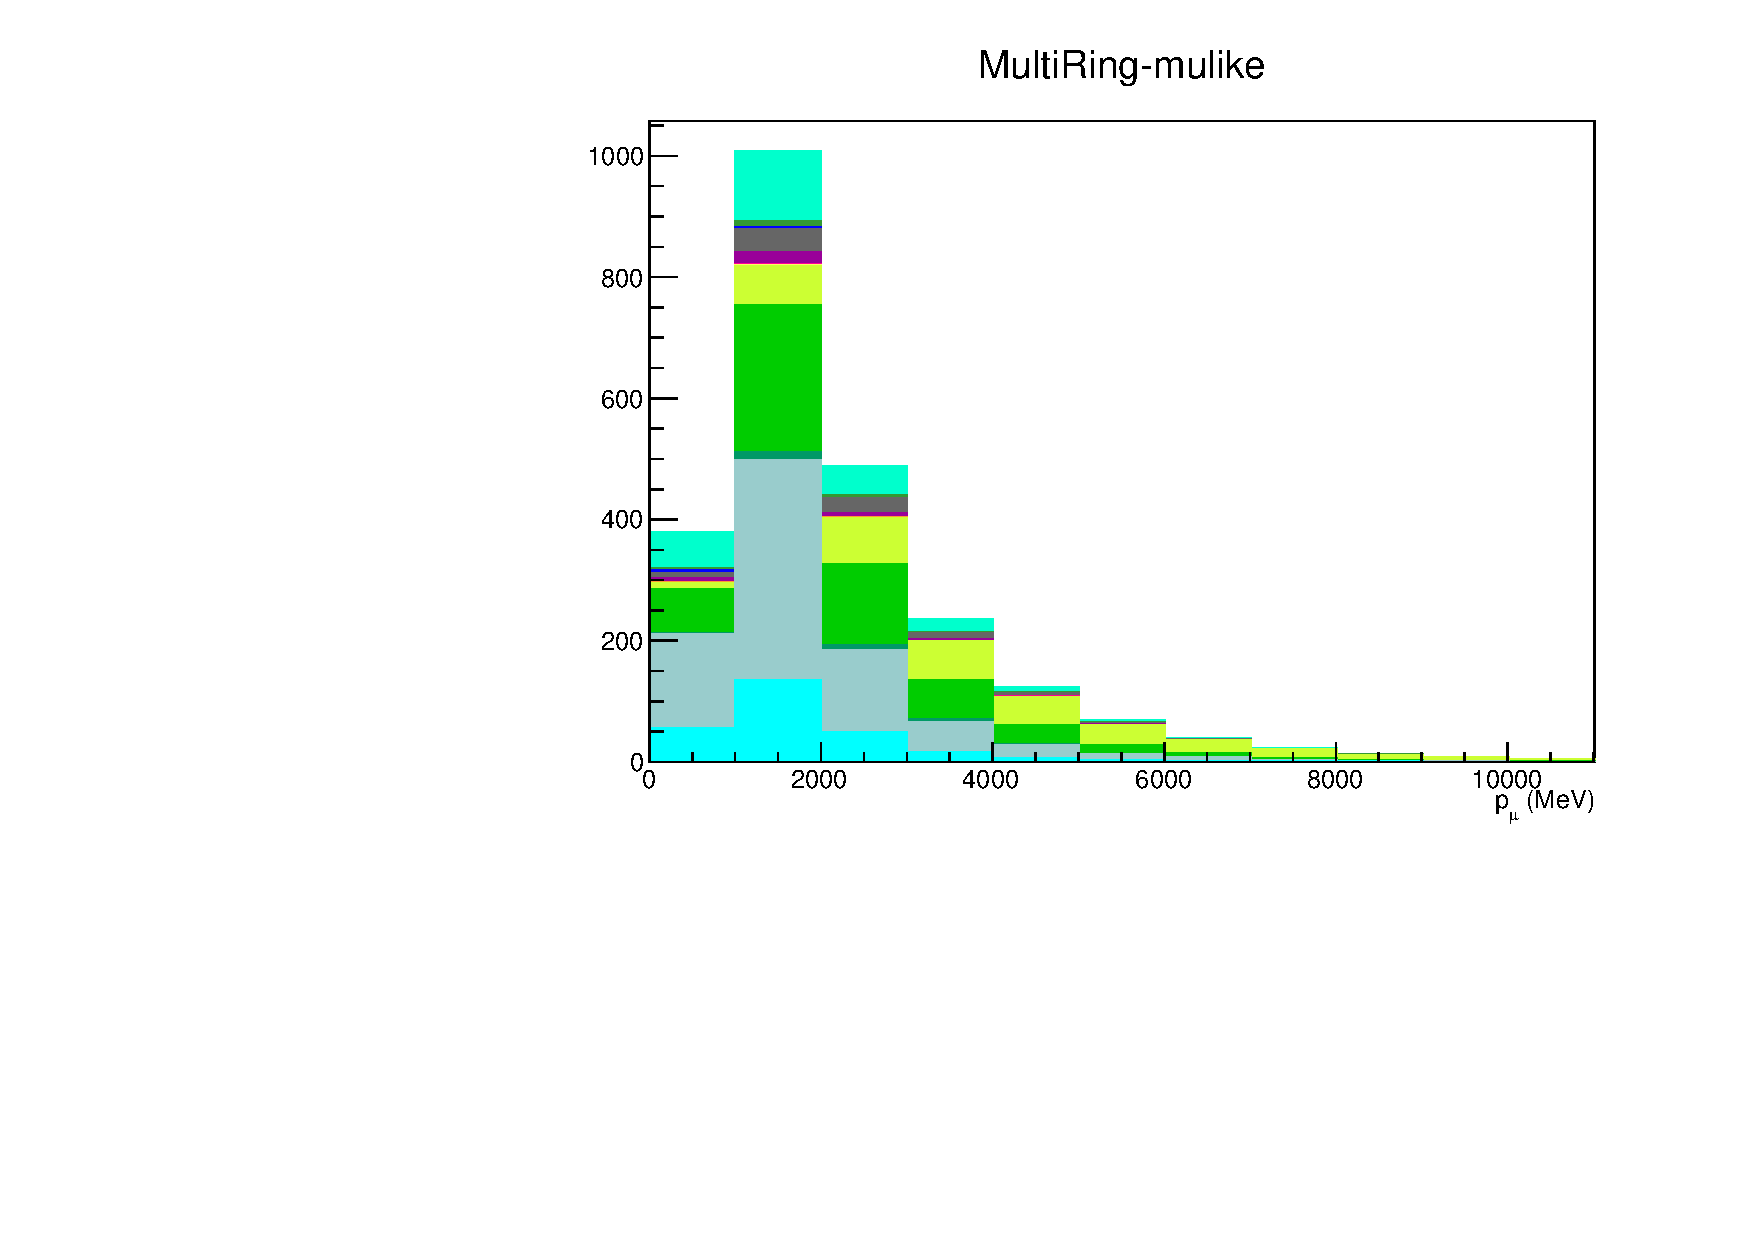
\includegraphics[width=\textwidth, trim= 0 0 0 30, clip]{Figures/Selections/AtmosphericByMode/MultiRing-mulike_LepMom.pdf}
    \caption{FC Multi-GeV multi-ring $\mu$-like}
    \end{subfigure}
    \begin{subfigure}[t]{0.49\textwidth}
    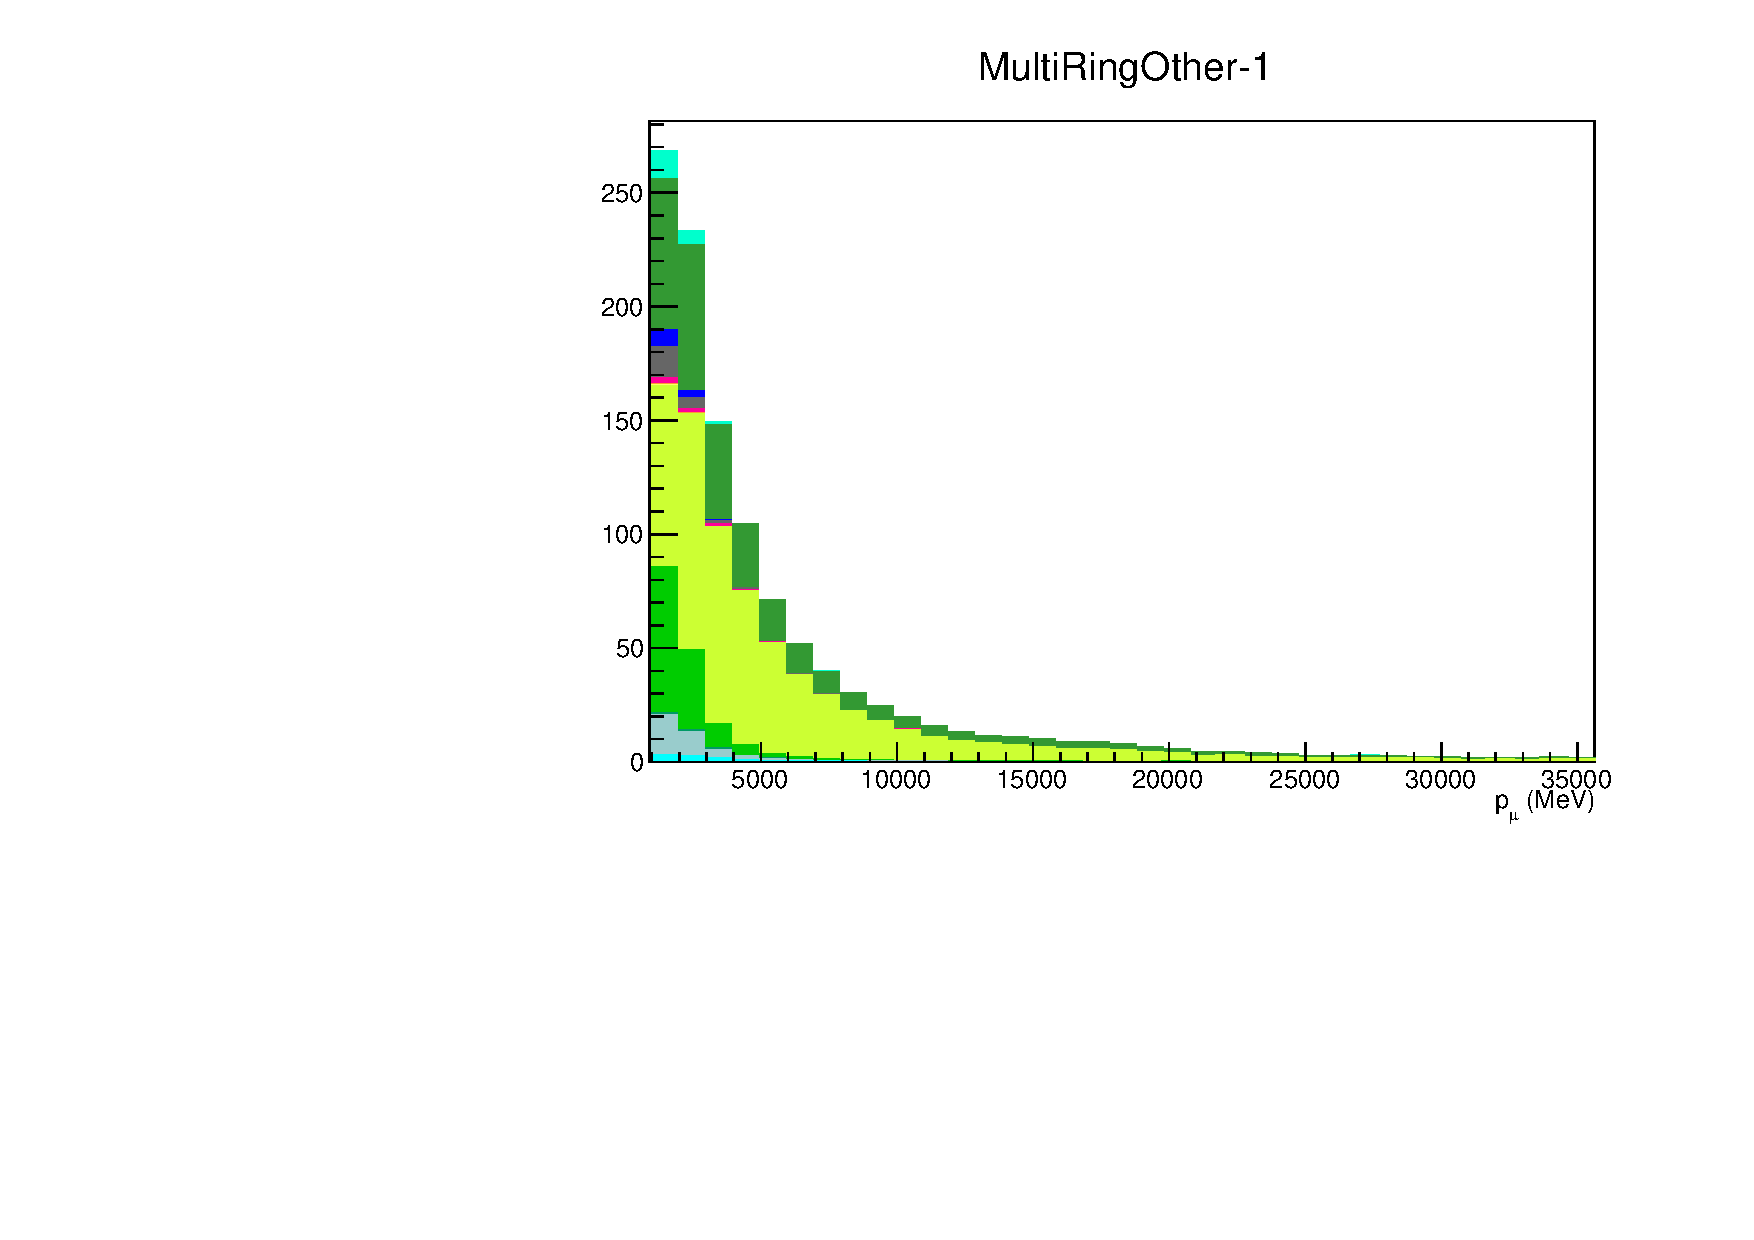
\includegraphics[width=\textwidth, trim= 0 0 0 30, clip]{Figures/Selections/AtmosphericByMode/MultiRingOther-1_LepMom.pdf}
    \caption{FC Multi-GeV multi-ring Other}
    \end{subfigure}
    \begin{subfigure}[t]{0.49\textwidth}
      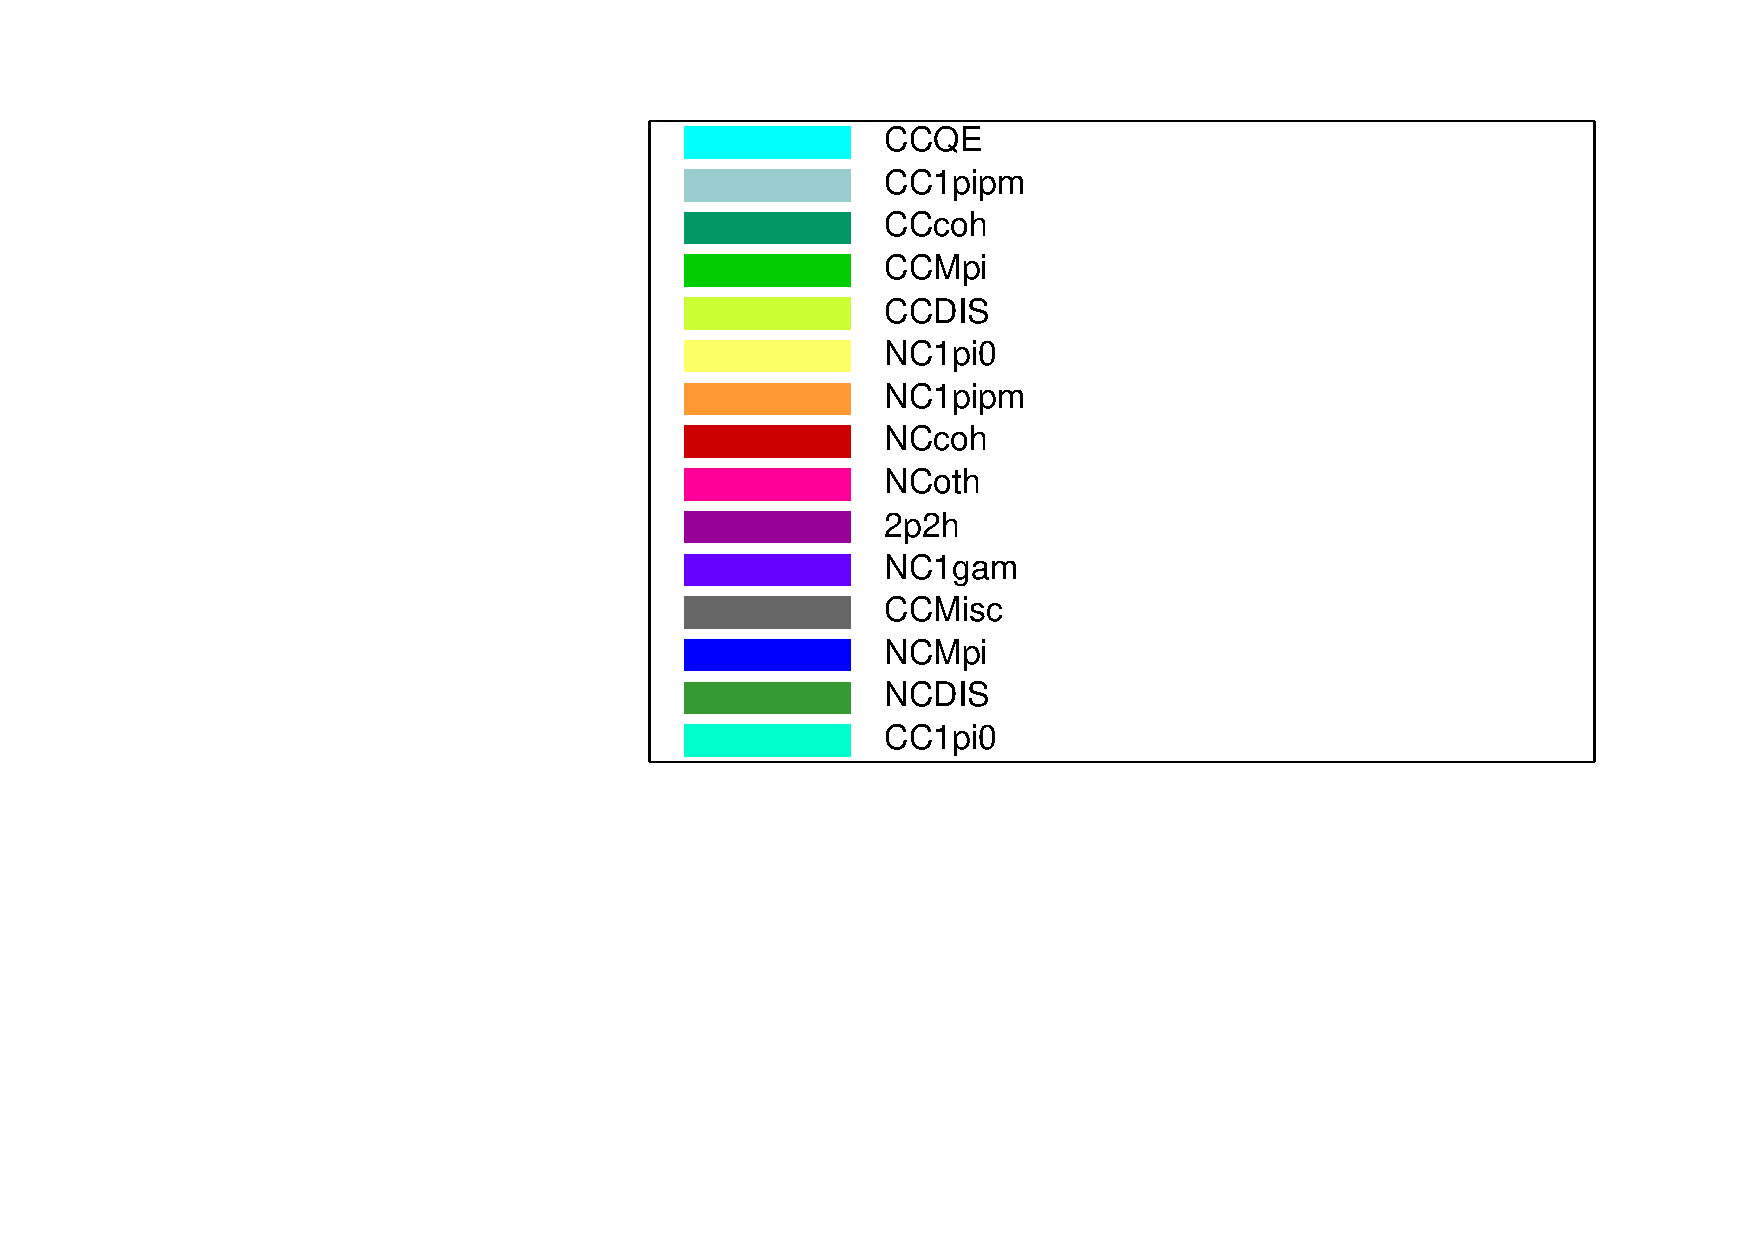
\includegraphics[page=1,width=\textwidth, trim= 0 0 0 30, clip]{Figures/Selections/AtmosphericByMode/Legend.pdf}
    \end{subfigure}
    
    \caption{Breakdown by interaction mode of the FC Multi-GeV  multi-ring atmospheric samples.}
    \label{fig:SKSamples:FCMultiRing}
\end{figure}

\clearpage
\section{Partially Contained Samples}
The breakdown for partially contained samples is highlighted in \autoref{fig:SKSamples:PC}. As with the multi-ring samples, there is no dominating interaction mode. The neutrino energies of events in this sample extend into the tens of GeV and become dominated by DIS interaction modes in the high energy limit.

\begin{figure}[ht]
    \begin{subfigure}[t]{0.49\textwidth}
    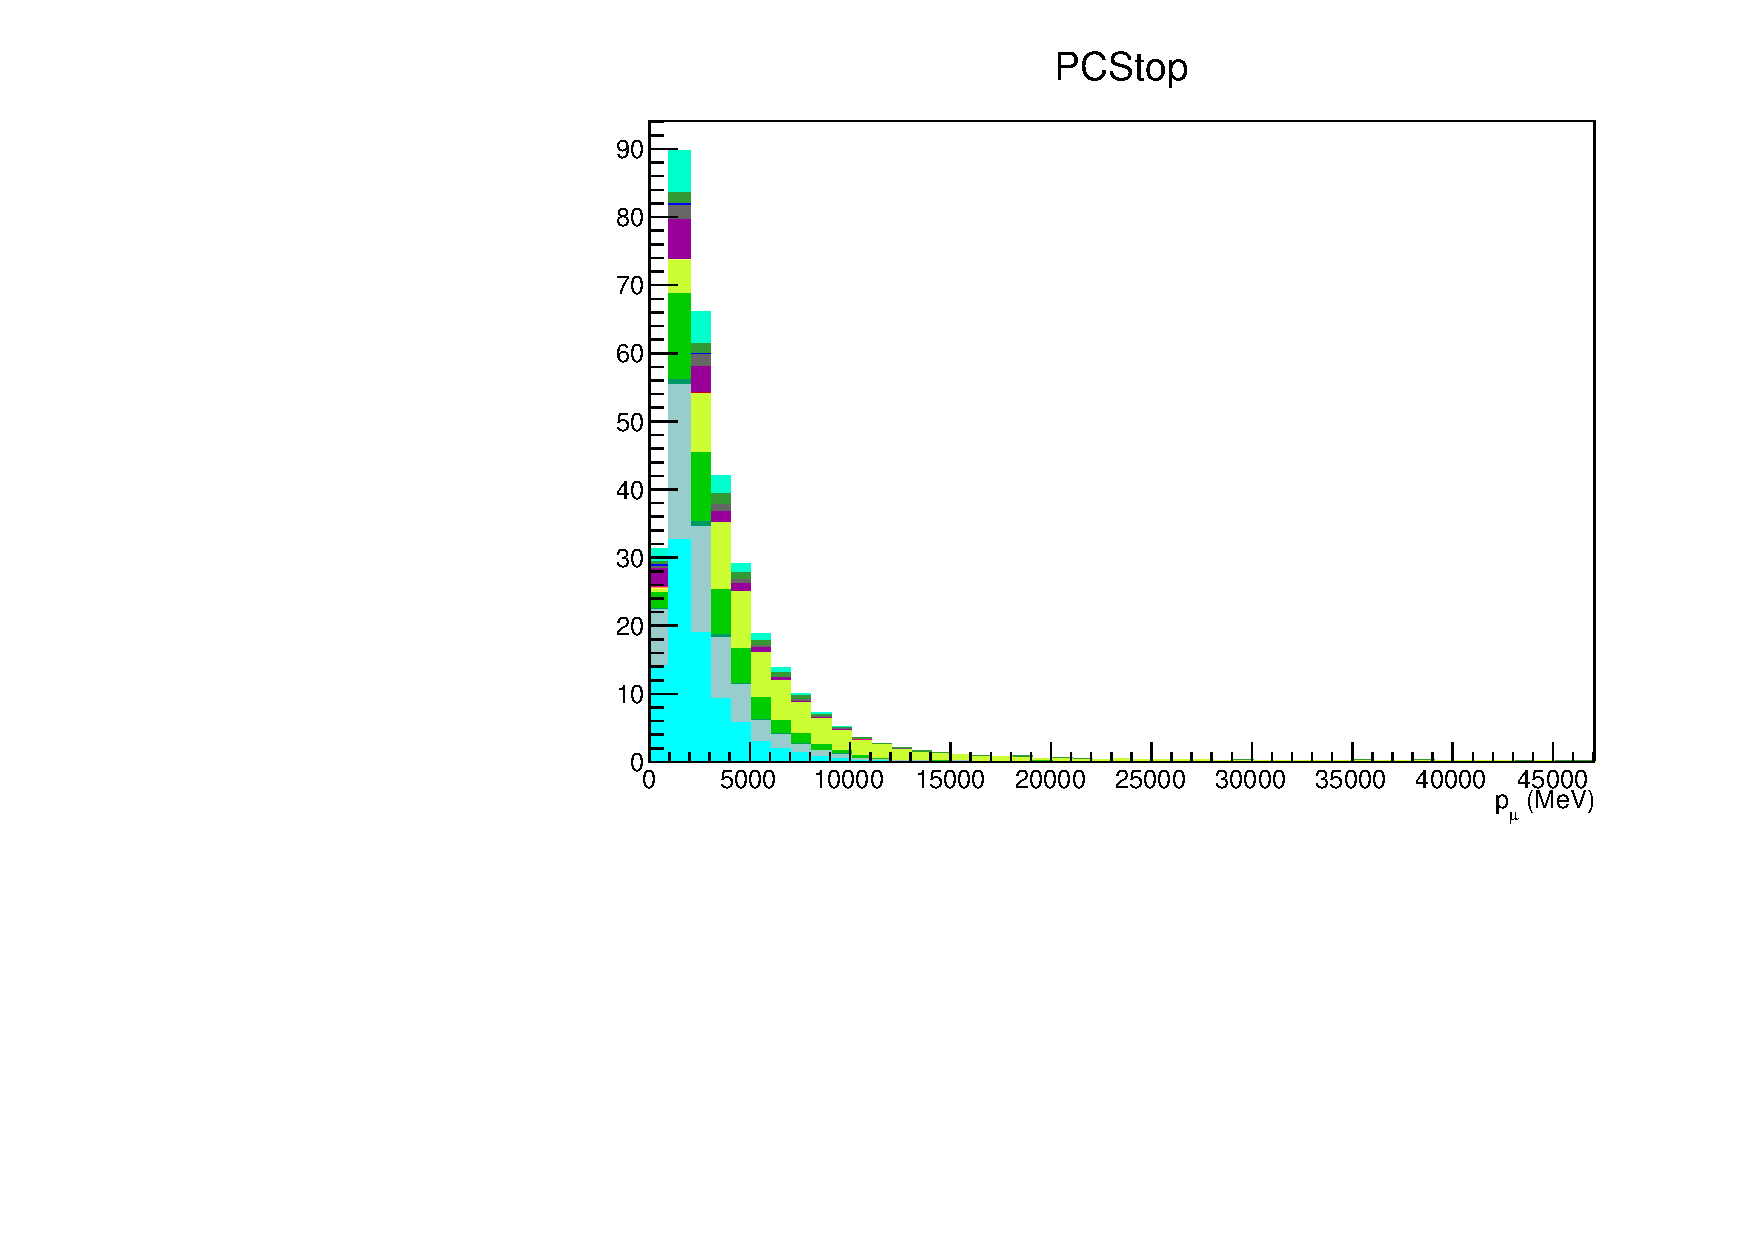
\includegraphics[width=\textwidth, trim= 0 0 0 30, clip]{Figures/Selections/AtmosphericByMode/PCStop_LepMom.pdf}
    \caption{PC stopping events}
    \end{subfigure}
    \begin{subfigure}[t]{0.49\textwidth}
    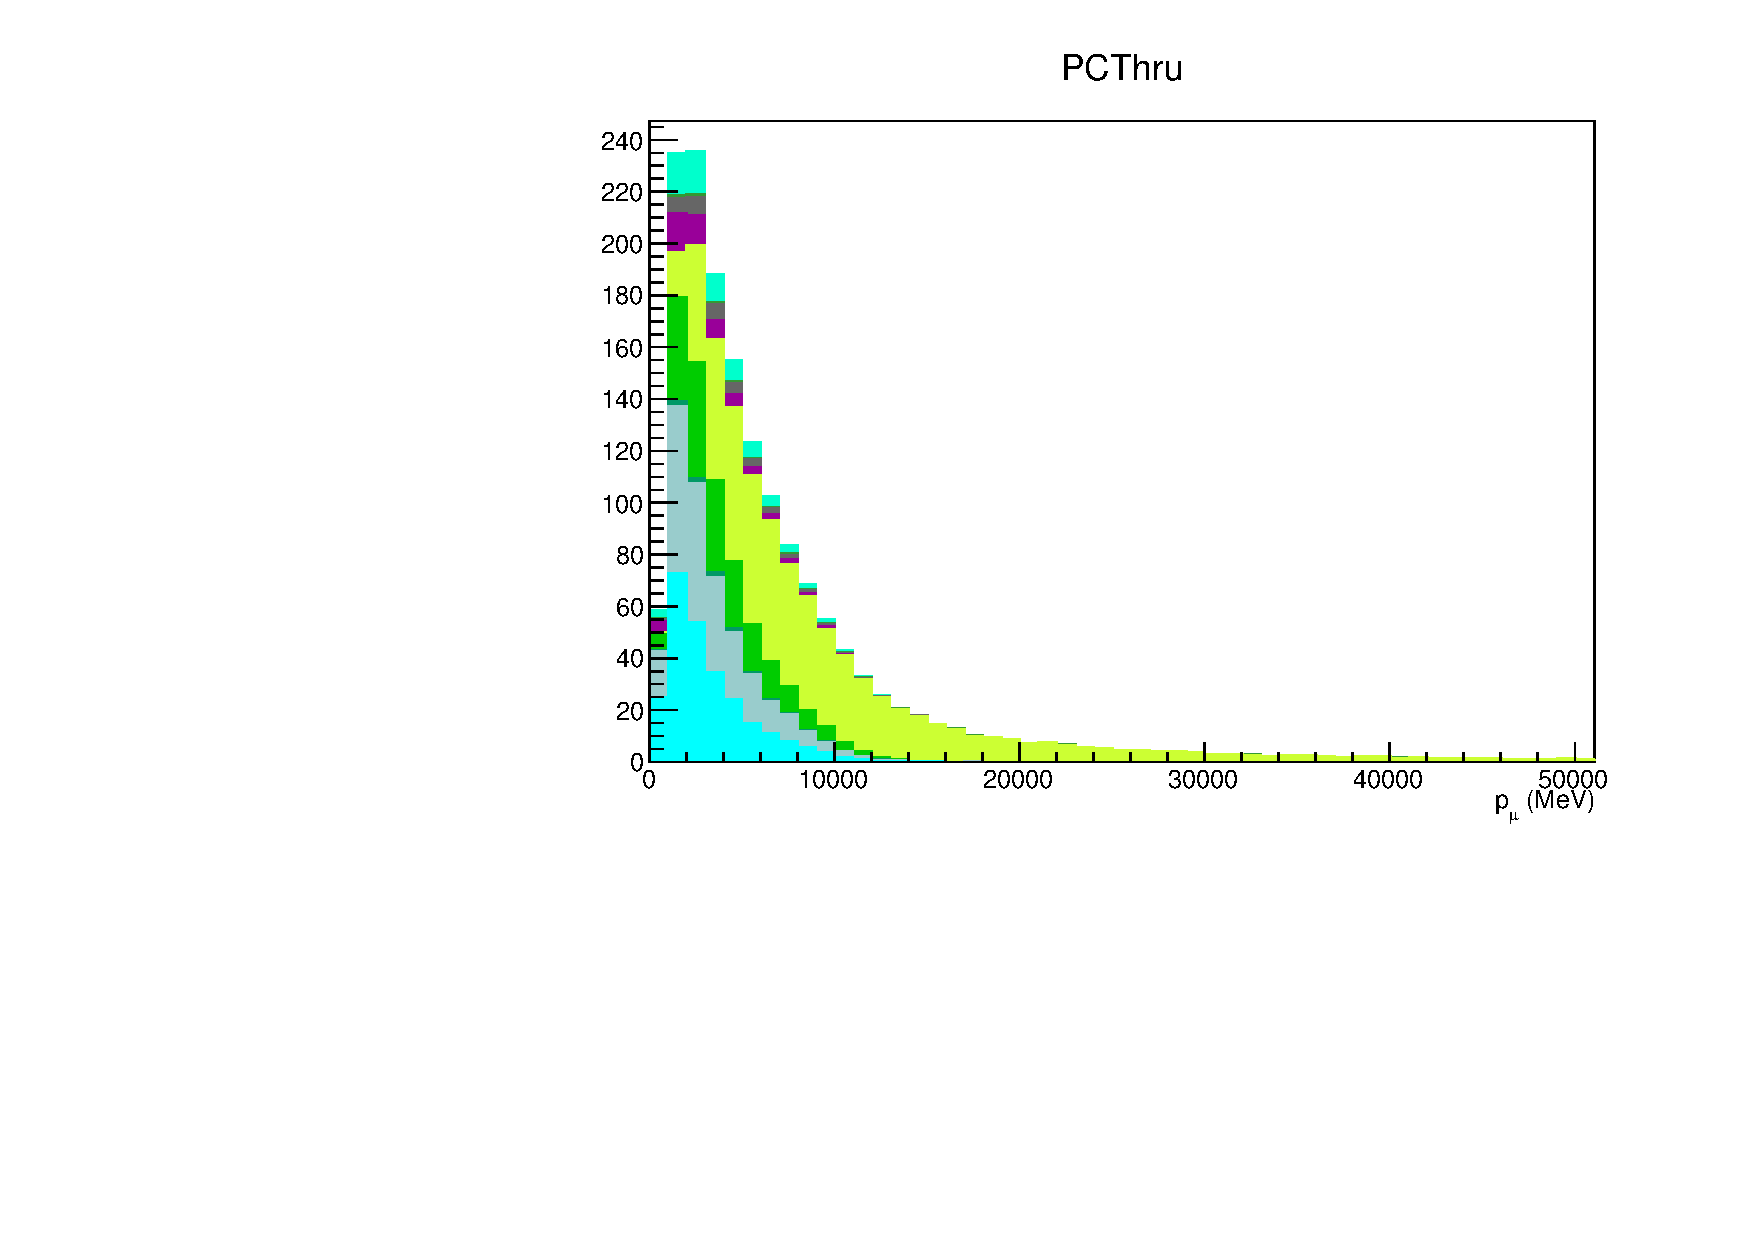
\includegraphics[width=\textwidth, trim= 0 0 0 30, clip]{Figures/Selections/AtmosphericByMode/PCThru_LepMom.pdf}
    \caption{PC through-going events.}
    \end{subfigure}
    \begin{subfigure}[t]{0.49\textwidth}
    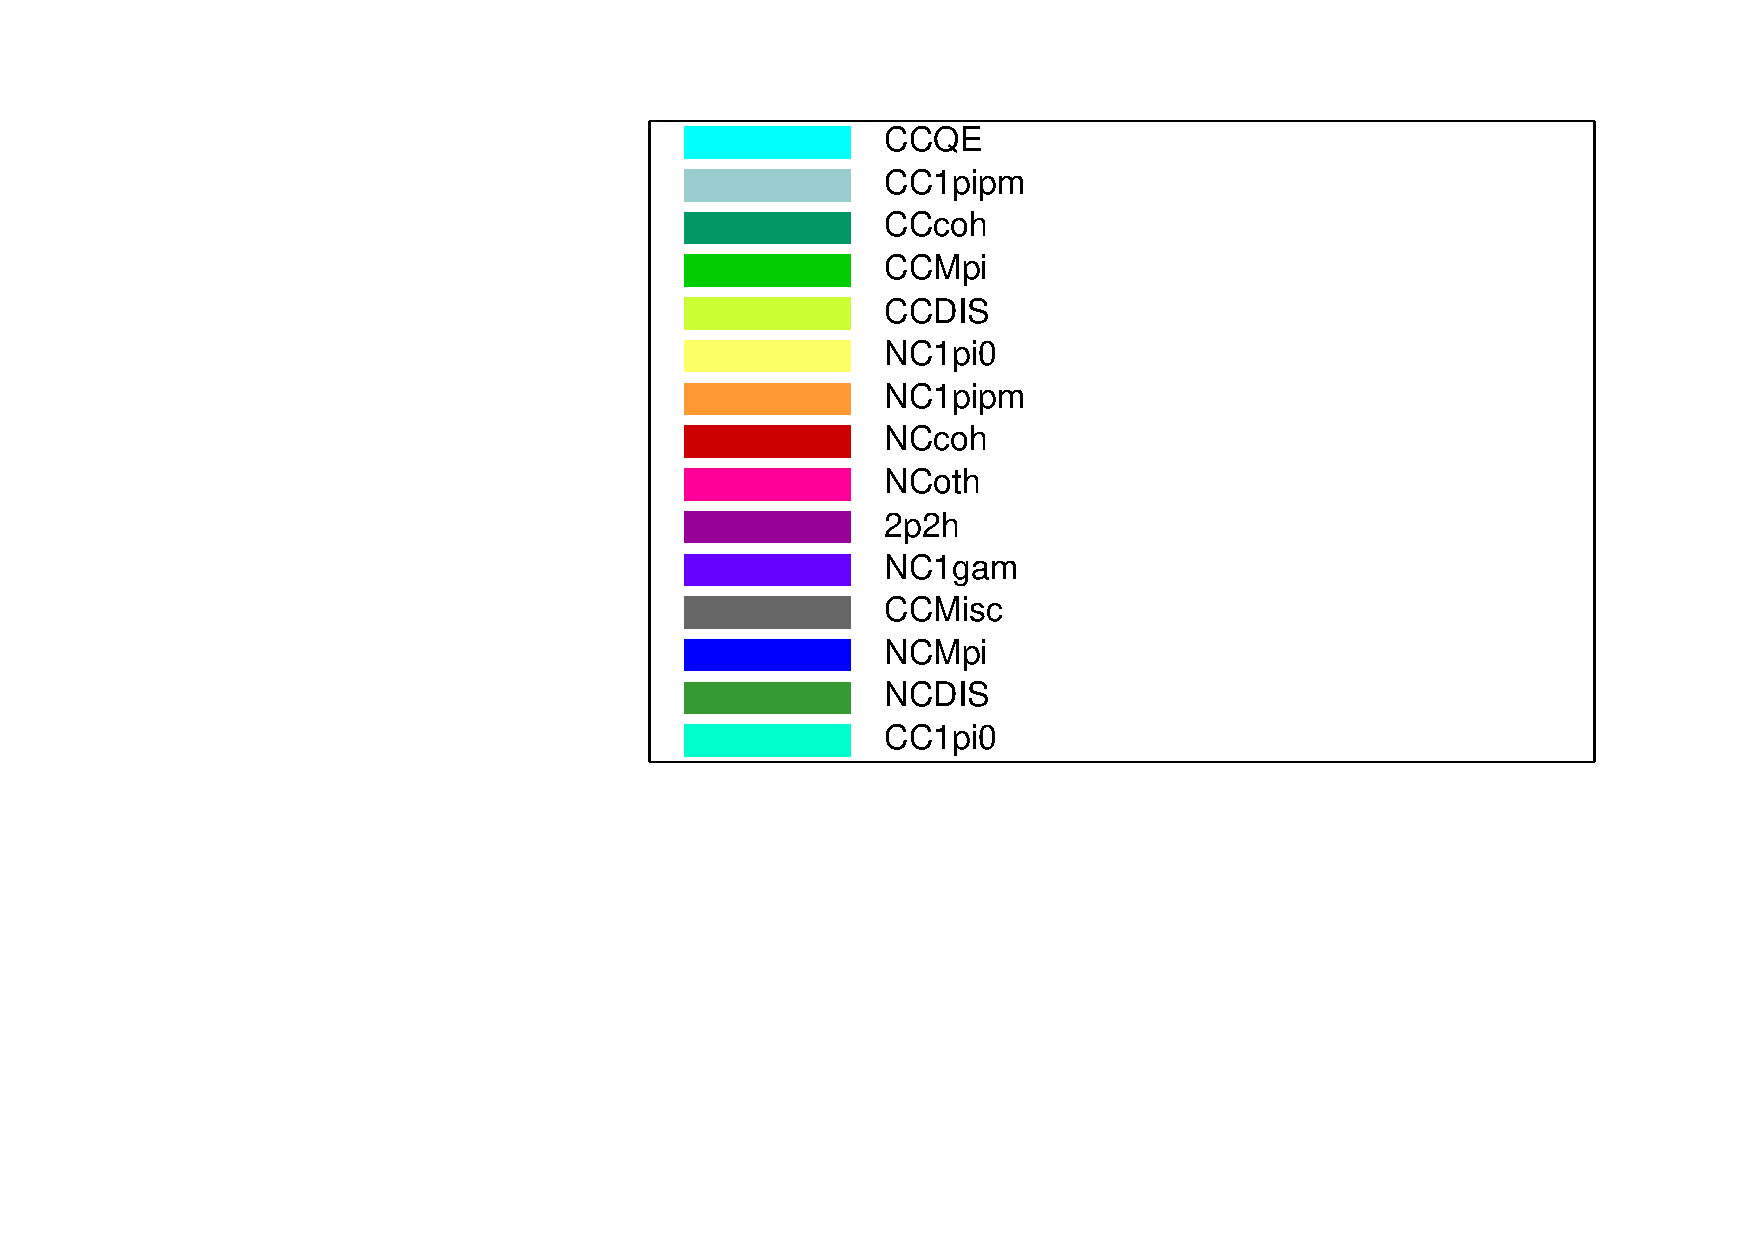
\includegraphics[page=1,width=\textwidth, trim= 0 0 0 30, clip]{Figures/Selections/AtmosphericByMode/Legend.pdf}
    \end{subfigure}
    
    \caption{Breakdown by interaction mode of the PC atmospheric samples.}
    \label{fig:SKSamples:PC}
\end{figure}

\clearpage
\section{Upward-Going Muon Samples}
The breakdown for upward-going muons is illustrated in \autoref{fig:SKSamples:Upmu}. These samples are significantly dominated by DIS interactions with energies extending up into the hundreds of GeV.

\begin{figure}[ht]
    \begin{subfigure}[t]{0.49\textwidth}
    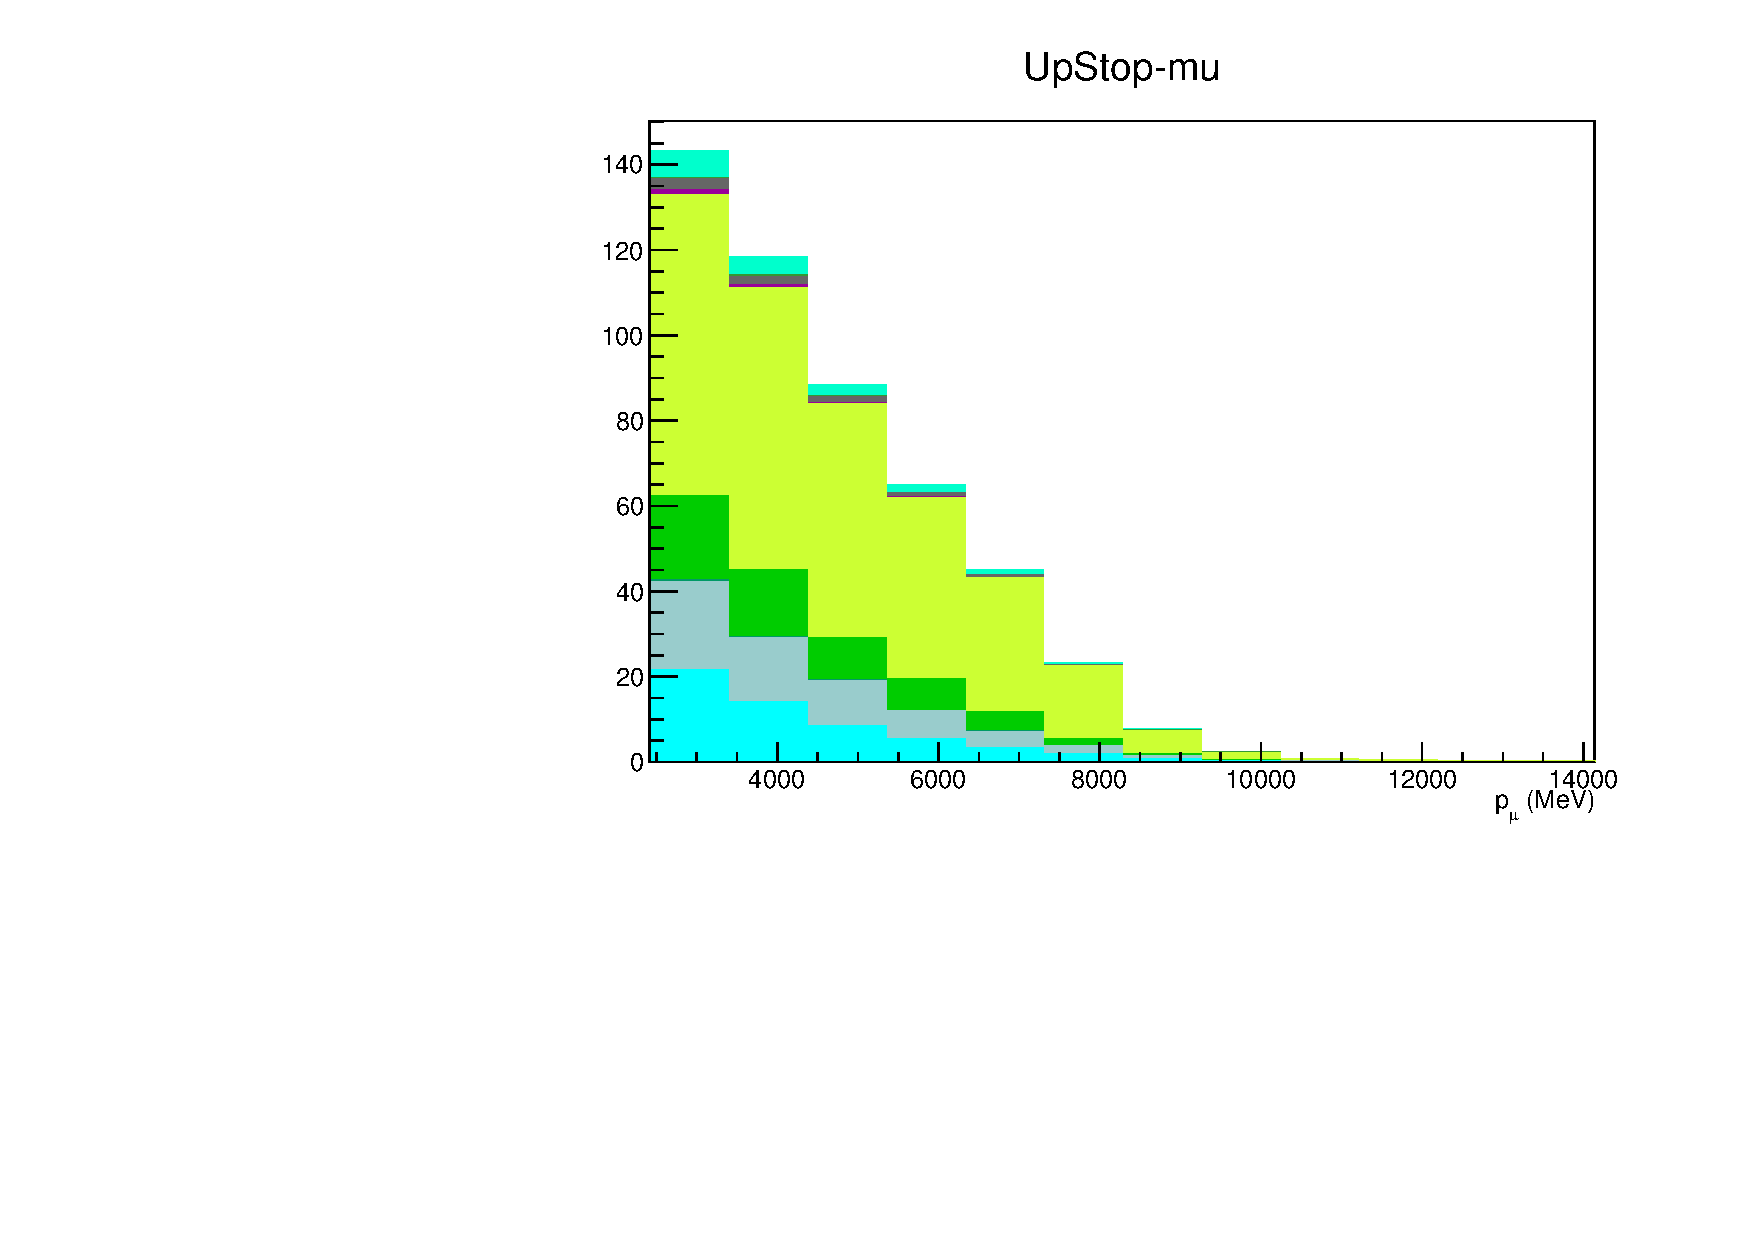
\includegraphics[width=\textwidth, trim= 0 0 0 30, clip]{Figures/Selections/AtmosphericByMode/UpStop-mu_LepMom.pdf}
    \caption{Up-$\mu$ stopping events}
    \end{subfigure}
    \begin{subfigure}[t]{0.49\textwidth}
    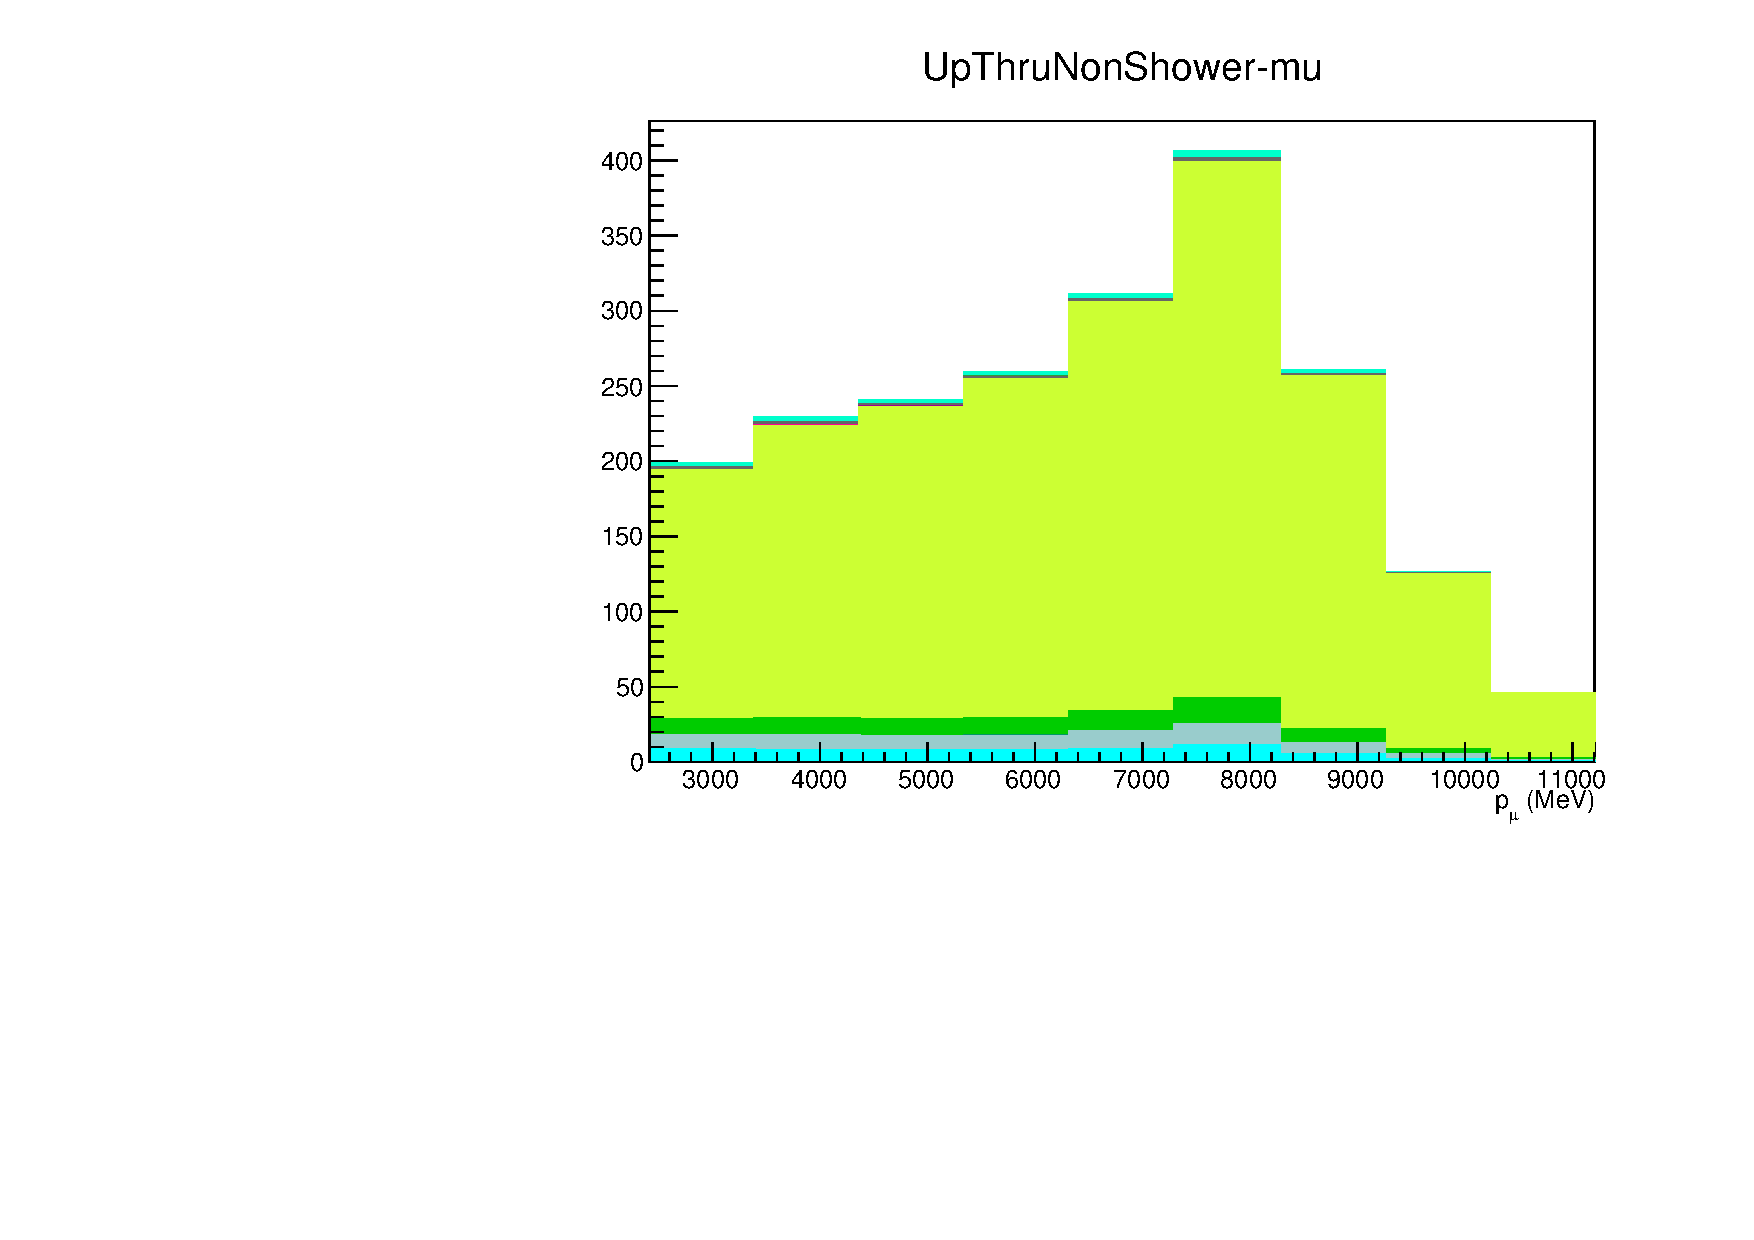
\includegraphics[width=\textwidth, trim= 0 0 0 30, clip]{Figures/Selections/AtmosphericByMode/UpThruNonShower-mu_LepMom.pdf}
    \caption{Up-$\mu$ through going non showering events}
    \end{subfigure}
    \begin{subfigure}[t]{0.49\textwidth}
    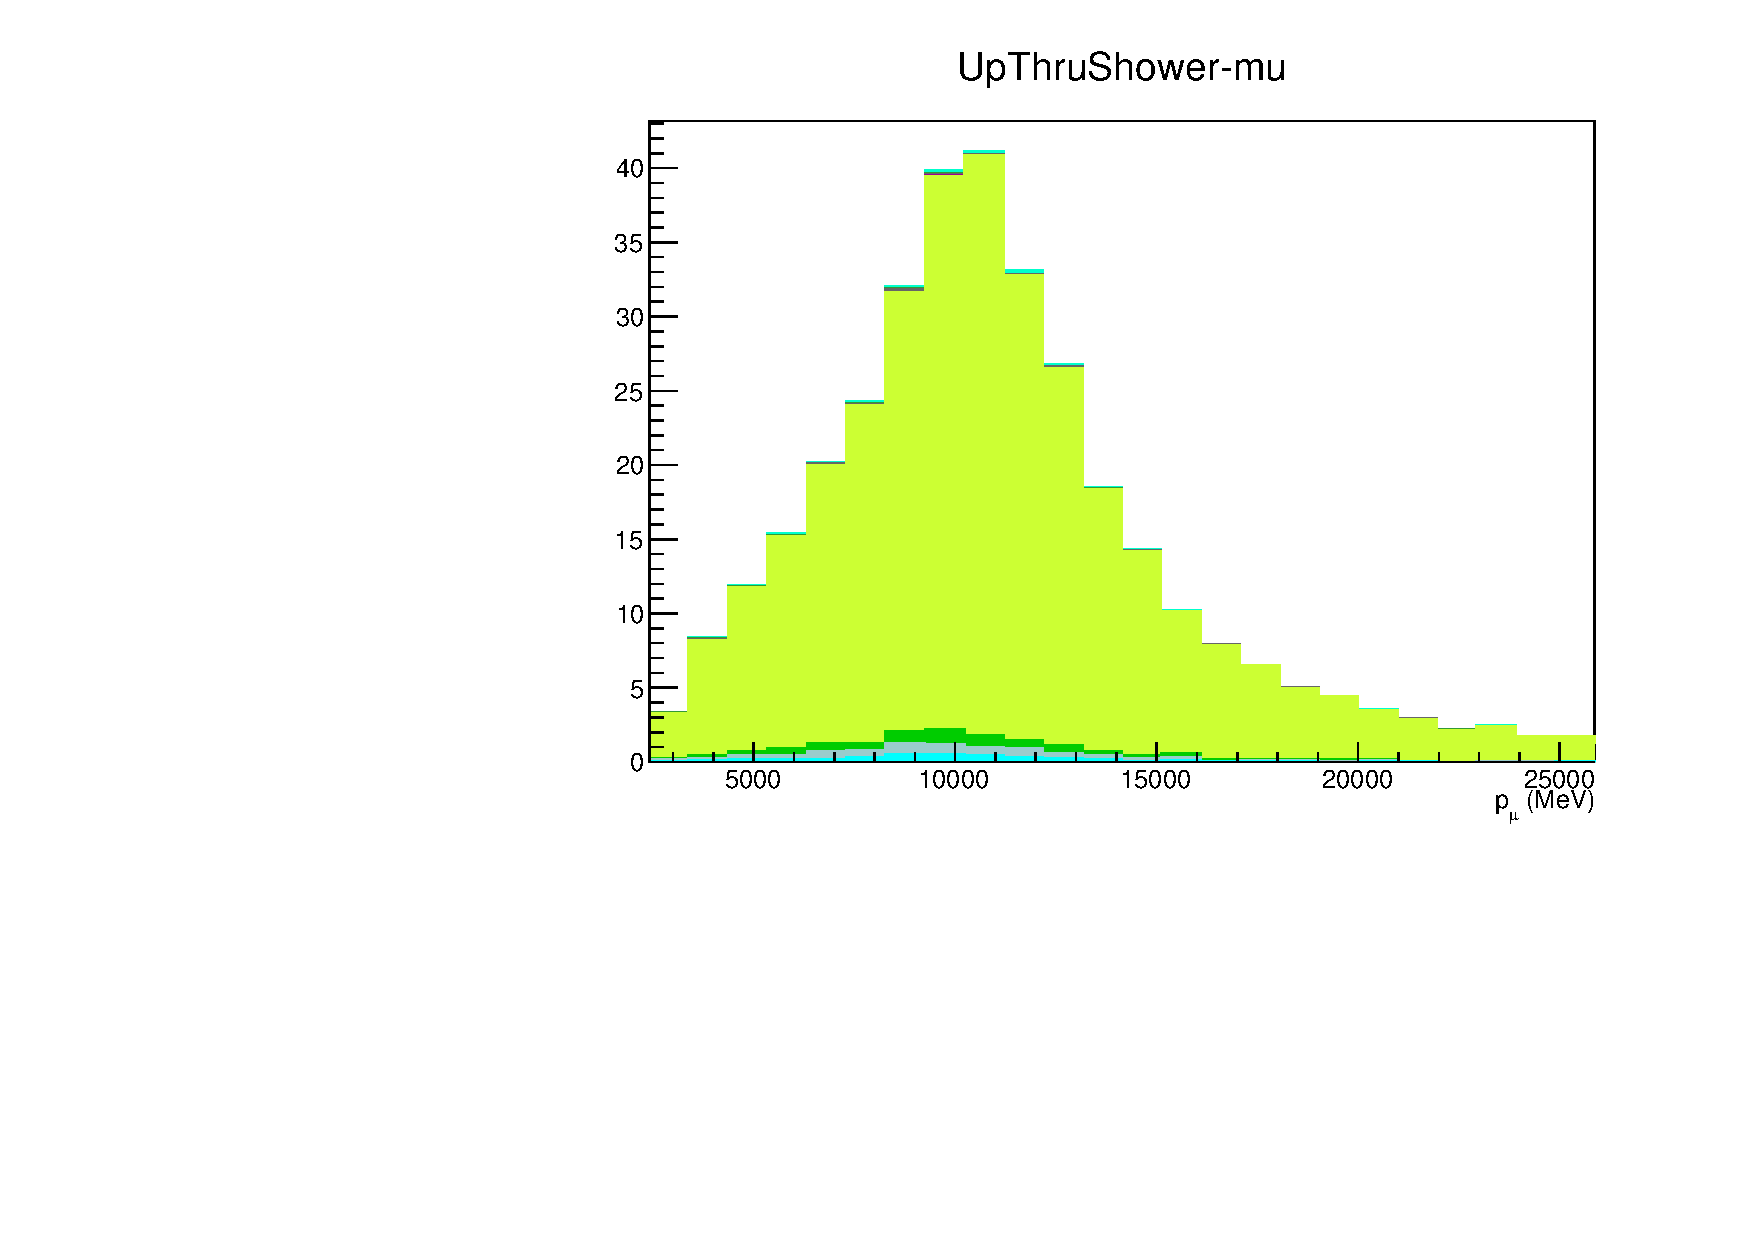
\includegraphics[width=\textwidth, trim= 0 0 0 30, clip]{Figures/Selections/AtmosphericByMode/UpThruShower-mu_LepMom.pdf}
    \caption{Up-$\mu$ through going showering events}
    \end{subfigure}
    \begin{subfigure}[t]{0.49\textwidth}
    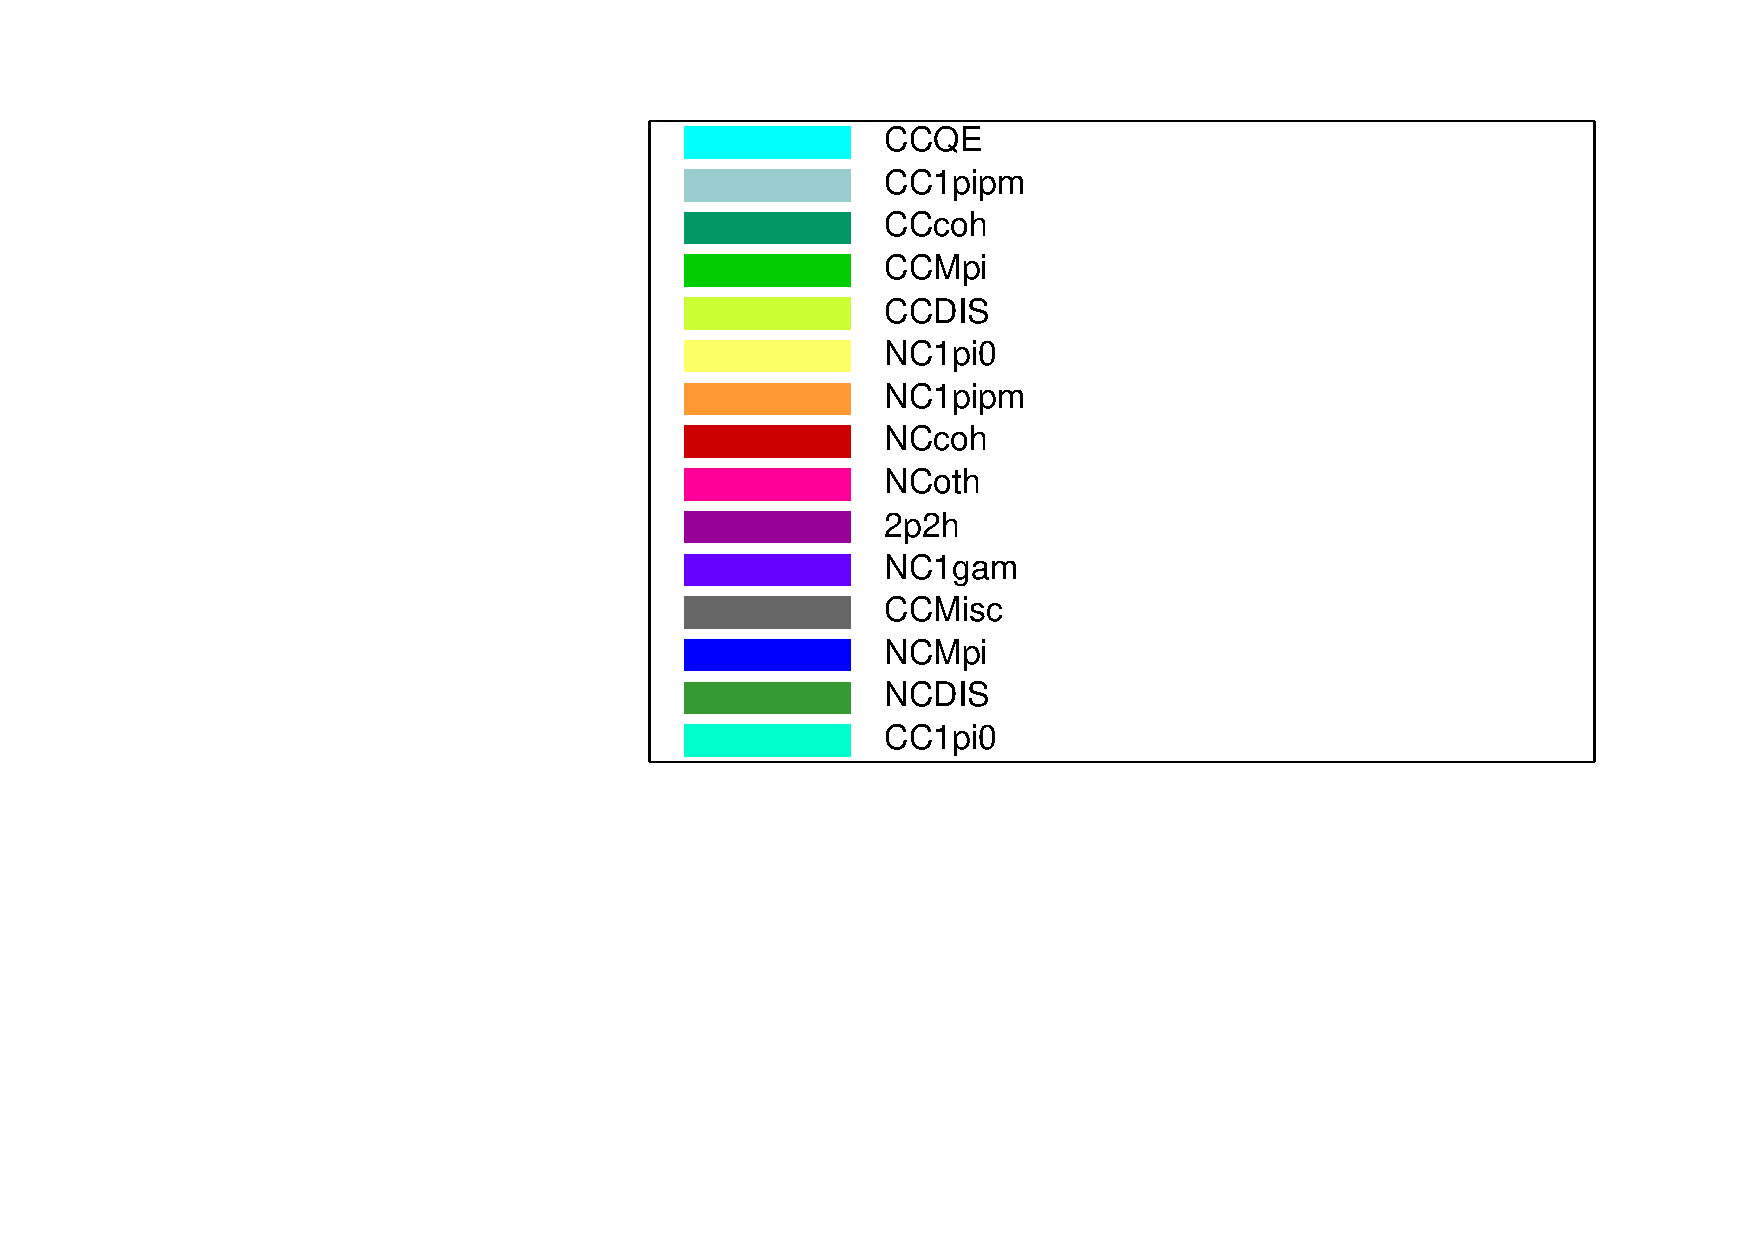
\includegraphics[width=\textwidth, page=1]{Figures/Selections/AtmosphericByMode/Legend.pdf}
    \end{subfigure}

    \caption{Breakdown by interaction mode of the atmospheric upward going muon samples.}
    \label{fig:SKSamples:Upmu}
\end{figure}

\end{appendices}

%% Produce the un-numbered back matter (e.g. colophon,
%% bibliography, tables of figures etc., index...)
\begin{backmatter}
  %\begin{colophon}
 % The end
%\end{colophon}

%% You're recommended to use the eprint-aware biblio styles which
%% can be obtained from e.g. www.arxiv.org. The file mythesis.bib
%% is derived from the source using the SPIRES Bibtex service.
\bibliographystyle{h-physrev}
%\bibliographystyle{plain}
%\bibliographystyle{apsrev4-1}
\bibliography{Thesis}

%% I prefer to put these tables here rather than making the
%% front matter seemingly interminable. No-one cares, anyway!
%\listoffigures
%\listoftables

%% If you have time and interest to generate a (decent) index,
%% then you've clearly spent more time on the write-up than the
%% research ;-)
%\printindex

\end{backmatter}

%% Close
\end{document}
